%% Run LaTeX on this file several times to get Table of Contents,
%% cross-references, and citations.

\documentclass[11pt]{book}
\usepackage{gvv-book}
\usepackage{gvv}
%\usepackage{Wiley-AuthoringTemplate}
\usepackage[sectionbib,authoryear]{natbib}% for name-date citation comment the below line
%\usepackage[sectionbib,numbers]{natbib}% for numbered citation comment the above line

%%********************************************************************%%
%%       How many levels of section head would you like numbered?     %%
%% 0= no section numbers, 1= section, 2= subsection, 3= subsubsection %%
\setcounter{secnumdepth}{3}
%%********************************************************************%%
%%**********************************************************************%%
%%     How many levels of section head would you like to appear in the  %%
%%				Table of Contents?			%%
%% 0= chapter, 1= section, 2= subsection, 3= subsubsection titles.	%%
\setcounter{tocdepth}{2}
%%**********************************************************************%%

%\includeonly{ch01}
\makeindex

\begin{document}

\frontmatter
%%%%%%%%%%%%%%%%%%%%%%%%%%%%%%%%%%%%%%%%%%%%%%%%%%%%%%%%%%%%%%%%
%% Title Pages
%% Wiley will provide title and copyright page, but you can make
%% your own titlepages if you'd like anyway
%% Setting up title pages, type in the appropriate names here:
\booktitle{The Navic Standard}

\subtitle{Through Python}

\AuAff{G. V. V. Sharma}


%% \\ will start a new line.
%% You may add \affil{} for affiliation, ie,
%\authors{Robert M. Groves\\
%\affil{Universitat de les Illes Balears}
%Floyd J. Fowler, Jr.\\
%\affil{University of New Mexico}
%}

%% Print Half Title and Title Page:
%\halftitlepage
\titlepage

%%%%%%%%%%%%%%%%%%%%%%%%%%%%%%%%%%%%%%%%%%%%%%%%%%%%%%%%%%%%%%%%
%% Copyright Page

\begin{copyrightpage}{2023}
%Title, etc
\end{copyrightpage}

% Note, you must use \ to start indented lines, ie,
% 
% \begin{copyrightpage}{2004}
% Survey Methodology / Robert M. Groves . . . [et al.].
% \       p. cm.---(Wiley series in survey methodology)
% \    ``Wiley-Interscience."
% \    Includes bibliographical references and index.
% \    ISBN 0-471-48348-6 (pbk.)
% \    1. Surveys---Methodology.  2. Social 
% \  sciences---Research---Statistical methods.  I. Groves, Robert M.  II. %
% Series.\\

% HA31.2.S873 2004
% 001.4'33---dc22                                             2004044064
% \end{copyrightpage}

%%%%%%%%%%%%%%%%%%%%%%%%%%%%%%%%%%%%%%%%%%%%%%%%%%%%%%%%%%%%%%%%
%% Only Dedication (optional) 

%\dedication{To my parents}

\tableofcontents

%\listoffigures %optional
%\listoftables  %optional

%% or Contributor Page for edited books
%% before \tableofcontents

%%%%%%%%%%%%%%%%%%%%%%%%%%%%%%%%%%%%%%%%%%%%%%%%%%%%%%%%%%%%%%%%
%  Contributors Page for Edited Book
%%%%%%%%%%%%%%%%%%%%%%%%%%%%%%%%%%%%%%%%%%%%%%%%%%%%%%%%%%%%%%%%

% If your book has chapters written by different authors,
% you'll need a Contributors page.

% Use \begin{contributors}...\end{contributors} and
% then enter each author with the \name{} command, followed
% by the affiliation information.

% \begin{contributors}
% \name{Masayki Abe,} Fujitsu Laboratories Ltd., Fujitsu Limited, Atsugi, Japan
%
% \name{L. A. Akers,} Center for Solid State Electronics Research, Arizona State University, Tempe, Arizona
%
% \name{G. H. Bernstein,} Department of Electrical and Computer Engineering, University of Notre Dame, Notre Dame, South Bend, Indiana; formerly of
% Center for Solid State Electronics Research, Arizona
% State University, Tempe, Arizona 
% \end{contributors}

%%%%%%%%%%%%%%%%%%%%%%%%%%%%%%%%%%%%%%%%%%%%%%%%%%%%%%%%%%%%%%%%
% Optional Foreword:

%\begin{foreword}
%\lipsum[1-2]
%\end{foreword}

%%%%%%%%%%%%%%%%%%%%%%%%%%%%%%%%%%%%%%%%%%%%%%%%%%%%%%%%%%%%%%%%
% Optional Preface:

%\begin{preface}
%\lipsum[1-1]
%\prefaceauthor{}
%\where{place\\
% date}
%\end{preface}

% ie,
% \begin{preface}
% This is an example preface.
% \prefaceauthor{R. K. Watts}
% \where{Durham, North Carolina\\
% September, 2004}

%%%%%%%%%%%%%%%%%%%%%%%%%%%%%%%%%%%%%%%%%%%%%%%%%%%%%%%%%%%%%%%%
% Optional Acknowledgments:

%\acknowledgments
%\lipsum[1-2]
%\authorinitials{I. R. S.}  

%%%%%%%%%%%%%%%%%%%%%%%%%%%%%%%%
%% Glossary Type of Environment:

% \begin{glossary}
% \term{<term>}{<description>}
% \end{glossary}

%%%%%%%%%%%%%%%%%%%%%%%%%%%%%%%%
%\begin{acronyms}
%\acro{ASTA}{Arrivals See Time Averages}
%\acro{BHCA}{Busy Hour Call Attempts}
%\acro{BR}{Bandwidth Reservation}
%\acro{b.u.}{bandwidth unit(s)}
%\acro{CAC}{Call / Connection Admission Control}
%\acro{CBP}{Call Blocking Probability(-ies)}
%\acro{CCS}{Centum Call Seconds}
%\acro{CDTM}{Connection Dependent Threshold Model}
%\acro{CS}{Complete Sharing}
%\acro{DiffServ}{Differentiated Services}
%\acro{EMLM}{Erlang Multirate Loss Model}
%\acro{erl}{The Erlang unit of traffic-load}
%\acro{FIFO}{First in - First out}
%\acro{GB}{Global balance}
%\acro{GoS}{Grade of Service}
%\acro{ICT}{Information and Communication Technology}
%\acro{IntServ}{Integrated Services}
%\acro{IP}{Internet Protocol}
%\acro{ITU-T}{International Telecommunication Unit -- Standardization sector}
%\acro{LB}{Local balance}
%\acro{LHS}{Left hand side}
%\acro{LIFO}{Last in - First out}
%\acro{MMPP}{Markov Modulated Poisson Process}
%\acro{MPLS}{Multiple Protocol Labeling Switching}
%\acro{MRM}{Multi-Retry Model}
%\acro{MTM}{Multi-Threshold Model}
%\acro{PASTA}{Poisson Arrivals See Time Averages}
%\acro{PDF}{Probability Distribution Function}
%\acro{pdf}{probability density function}
%\acro{PFS}{Product Form Solution}
%\acro{QoS}{Quality of Service}
%\acro{r.v.}{random variable(s)}
%\acro{RED}{random early detection}
%\acro{RHS}{Right hand side}
%\acro{RLA}{Reduced Load Approximation}
%\acro{SIRO}{service in random order}
%\acro{SRM}{Single-Retry Model}
%\acro{STM}{Single-Threshold Model}
%\acro{TCP}{Transport Control Protocol}
%\acro{TH}{Threshold(s)}
%\acro{UDP}{User Datagram Protocol}
%\end{acronyms}

\setcounter{page}{1}

\begin{introduction}
This book introduces the NAVIC communication standard through Python exercises
\end{introduction}
\mainmatter
\chapter{Design Parameters}
\section{The Frequency Bands}
	\begin{figure}[!ht]
	\centering
	\tikzset{every picture/.style={line width=0.75pt}} %set default line width to 0.75pt        
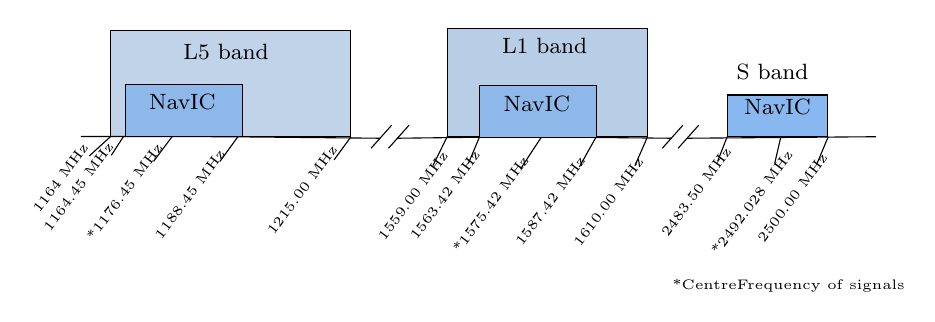
\begin{tikzpicture}[x=0.75pt,y=0.75pt,yscale=-1,xscale=1]
%uncomment if require: \path (0,471); %set diagram left start at 0, and has height of 471

%Shape: Rectangle [id:dp9517205987034671] 
\draw  [fill={rgb, 255:red, 192; green, 211; blue, 233 }  ,fill opacity=1 ] (92.53,176.6) -- (208.12,176.6) -- (208.12,227.79) -- (92.53,227.79) -- cycle ;
%Shape: Rectangle [id:dp3424557357689655] 
\draw  [fill={rgb, 255:red, 184; green, 205; blue, 230 }  ,fill opacity=1 ] (254.8,175.52) -- (351.33,175.52) -- (351.33,227.79) -- (254.8,227.79) -- cycle ;
%Shape: Rectangle [id:dp8560354037740456] 
\draw  [fill={rgb, 255:red, 137; green, 183; blue, 239 }  ,fill opacity=1 ] (389.7,207.67) -- (438,207.67) -- (438,227.79) -- (389.7,227.79) -- cycle ;
%Straight Lines [id:da4982550625943454] 
\draw    (78.33,227.67) -- (148.8,227.79) ;
%Straight Lines [id:da09038165069225701] 
\draw    (148.8,227.79) -- (222.43,228.52) ;
%Straight Lines [id:da6963693922945375] 
\draw    (230.82,228.52) -- (290.62,227.79) ;
%Straight Lines [id:da5101605840021868] 
\draw    (290.62,227.79) -- (362.75,228.52) ;
%Straight Lines [id:da4455724073590175] 
\draw    (218.13,233.34) -- (222.43,228.52) -- (228.04,222.24) ;
%Straight Lines [id:da44617587453109] 
\draw    (370.38,228.52) -- (461.33,227.79) ;
%Shape: Rectangle [id:dp9436860161134495] 
\draw  [fill={rgb, 255:red, 142; green, 184; blue, 233 }  ,fill opacity=1 ] (99.9,202.67) -- (156.33,202.67) -- (156.33,227.7) -- (99.9,227.7) -- cycle ;
%Straight Lines [id:da1306791733179924] 
\draw    (226.51,233.34) -- (230.82,228.52) -- (236.42,222.24) ;
%Straight Lines [id:da9755728827987384] 
\draw    (358.45,233.34) -- (362.75,228.52) -- (368.36,222.24) ;
%Straight Lines [id:da6153463426480046] 
\draw    (366.07,233.34) -- (370.38,228.52) -- (375.98,222.24) ;
%Straight Lines [id:da524212389543216] 
\draw    (92.53,227.79) -- (82.36,237.05) ;
%Straight Lines [id:da6359631954084011] 
\draw    (98.83,227.7) -- (92.93,236.8) ;
%Straight Lines [id:da4309637537474662] 
\draw    (122.33,227.67) -- (113.33,239.67) ;
%Straight Lines [id:da7084848716058743] 
\draw    (154.02,227.7) -- (145.34,239.67) ;
%Straight Lines [id:da9025278744467291] 
\draw    (208.45,227.79) -- (200.32,238.9) ;
%Straight Lines [id:da4288601859090342] 
\draw    (254.8,227.79) -- (247.94,241.67) ;
%Straight Lines [id:da6434353112428917] 
\draw    (270.26,228.16) -- (265,240.67) ;
%Straight Lines [id:da6934497348254585] 
\draw    (299.96,228.29) -- (290.19,243.19) ;
%Straight Lines [id:da08356280974055585] 
\draw    (326.33,228.29) -- (318.52,242.26) ;
%Straight Lines [id:da47170852835093413] 
\draw    (389.7,227.79) -- (385.12,239.51) ;
%Straight Lines [id:da39211419648473833] 
\draw    (415.47,228.16) -- (412.56,240.75) ;
%Straight Lines [id:da6629675504582904] 
\draw    (438.38,227.79) -- (433,240.67) ;
%Straight Lines [id:da16092426119270775] 
\draw    (351.33,227.79) -- (345.23,241.76) ;
%Shape: Rectangle [id:dp5224743842810824] 
\draw  [fill={rgb, 255:red, 142; green, 184; blue, 233 }  ,fill opacity=1 ] (270.26,203.12) -- (326.69,203.12) -- (326.69,228.16) -- (270.26,228.16) -- cycle ;

% Text Node
\draw (393.01,191.59) node [anchor=north west][inner sep=0.75pt]   [align=left] {{\footnotesize S band}};
% Text Node
\draw (396.7,208.67) node [anchor=north west][inner sep=0.75pt]   [align=left] {{\footnotesize NavIC}};
% Text Node
\draw (279.94,179.23) node [anchor=north west][inner sep=0.75pt]  [font=\footnotesize] [align=left] {L1 band};
% Text Node
%\draw (100.68,152.4) node [anchor=north west][inner sep=0.75pt]  [font=\scriptsize] [align=left] {ARNS / RNSS Band};
% Text Node
\draw (126.47,182.01) node [anchor=north west][inner sep=0.75pt]  [font=\footnotesize] [align=left] {L5 band};
% Text Node
\draw (109.89,206.05) node [anchor=north west][inner sep=0.75pt]   [align=left] {{\footnotesize NavIC}};
% Text Node
\draw (280.67,206.99) node [anchor=north west][inner sep=0.75pt]  [font=\normalsize] [align=left] {{\footnotesize NavIC}};
% Text Node
%\draw (252.7,152.4) node [anchor=north west][inner sep=0.75pt]  [font=\scriptsize] [align=left] {ARNS / RNSS Band};
% Text Node
%\draw (367.49,152.32) node [anchor=north west][inner sep=0.75pt]  [font=\scriptsize] [align=left] {RNSS/RDSS Band};
% Text Node
\draw (52.94,262.5) node [anchor=north west][inner sep=0.75pt]  [font=\scriptsize,rotate=-306.7] [align=left] {{\tiny 1164 MHz}};
% Text Node
\draw (58.07,271.48) node [anchor=north west][inner sep=0.75pt]  [font=\scriptsize,rotate=-306.7] [align=left] {{\tiny 1164.45 MHz}};
% Text Node
\draw (78.65,275.41) node [anchor=north west][inner sep=0.75pt]  [font=\scriptsize,rotate=-306.7] [align=left] {{\tiny *1176.45 MHz}};
% Text Node
\draw (111.71,275.12) node [anchor=north west][inner sep=0.75pt]  [font=\scriptsize,rotate=-306.7] [align=left] {{\tiny 1188.45 MHz}};
% Text Node
\draw (165.87,273.01) node [anchor=north west][inner sep=0.75pt]  [font=\scriptsize,rotate=-306.7] [align=left] {{\tiny 1215.00 MHz}};
% Text Node
\draw (219.28,275.78) node [anchor=north west][inner sep=0.75pt]  [font=\scriptsize,rotate=-306.7] [align=left] {{\tiny 1559.00 MHz}};
% Text Node
\draw (234.71,275.48) node [anchor=north west][inner sep=0.75pt]  [font=\scriptsize,rotate=-306.7] [align=left] {{\tiny 1563.42 MHz}};
% Text Node
\draw (255.1,281.42) node [anchor=north west][inner sep=0.75pt]  [font=\scriptsize,rotate=-306.7] [align=left] {{\tiny *1575.42 MHz}};
% Text Node
\draw (285.46,278.33) node [anchor=north west][inner sep=0.75pt]  [font=\scriptsize,rotate=-306.7] [align=left] {{\tiny 1587.42 MHz}};
% Text Node
\draw (313.45,278.62) node [anchor=north west][inner sep=0.75pt]  [font=\scriptsize,rotate=-306.7] [align=left] {{\tiny 1610.00 MHz}};
% Text Node
\draw (355.7,273.93) node [anchor=north west][inner sep=0.75pt]  [font=\scriptsize,rotate=-306.7] [align=left] {{\tiny 2483.50 MHz}};
% Text Node
\draw (379.59,282.47) node [anchor=north west][inner sep=0.75pt]  [font=\scriptsize,rotate=-306.7] [align=left] {{\tiny *2492.028 MHz}};
% Text Node
\draw (402.14,276.71) node [anchor=north west][inner sep=0.75pt]  [font=\scriptsize,rotate=-306.7] [align=left] {{\tiny 2500.00 MHz}};
% Text Node
\draw (362,295) node [anchor=north west][inner sep=0.75pt]  [font=\tiny] [align=left] {{\tiny *CentreFrequency of signals}};

\end{tikzpicture}

	\caption{Frequency bands of NavIC Signals}
	\label{figure:bandsfig}
	\end{figure}

\begin{table}[!ht]
	\small
	\centering
	%\subimport{table/}{table1.tex}
	%%%%%%%%%%%%%%%%%%%%%%%%%%%%%%%%%%%%%%%%%%%%%%%%%%%%%%%%%%%%%%%%%%%%%%
%%                                                                  %%
%%  This is the header of a LaTeX2e file exported from Gnumeric.    %%
%%                                                                  %%
%%  This file can be compiled as it stands or included in another   %%
%%  LaTeX document. The table is based on the longtable package so  %%
%%  the longtable options (headers, footers...) can be set in the   %%
%%  preamble section below (see PRAMBLE).                           %%
%%                                                                  %%
%%  To include the file in another, the following two lines must be %%
%%  in the including file:                                          %%
%%        \def\inputGnumericTable{}                                 %%
%%  at the beginning of the file and:                               %%
%%        \input{name-of-this-file.tex}                             %%
%%  where the table is to be placed. Note also that the including   %%
%%  file must use the following packages for the table to be        %%
%%  rendered correctly:                                             %%
%%    \usepackage[latin1]{inputenc}                                 %%
%%    \usepackage{color}                                            %%
%%    \usepackage{array}                                            %%
%%    \usepackage{longtable}                                        %%
%%    \usepackage{calc}                                             %%
%%    \usepackage{multirow}                                         %%
%%    \usepackage{hhline}                                           %%
%%    \usepackage{ifthen}                                           %%
%%  optionally (for landscape tables embedded in another document): %%
%%    \usepackage{lscape}                                           %%
%%                                                                  %%
%%%%%%%%%%%%%%%%%%%%%%%%%%%%%%%%%%%%%%%%%%%%%%%%%%%%%%%%%%%%%%%%%%%%%%



%%  This section checks if we are begin input into another file or  %%
%%  the file will be compiled alone. First use a macro taken from   %%
%%  the TeXbook ex 7.7 (suggestion of Han-Wen Nienhuys).            %%
\def\ifundefined#1{\expandafter\ifx\csname#1\endcsname\relax}


%%  Check for the \def token for inputed files. If it is not        %%
%%  defined, the file will be processed as a standalone and the     %%
%%  preamble will be used.                                          %%
\ifundefined{inputGnumericTable}

%%  We must be able to close or not the document at the end.        %%
	\def\gnumericTableEnd{\end{document}}


%%%%%%%%%%%%%%%%%%%%%%%%%%%%%%%%%%%%%%%%%%%%%%%%%%%%%%%%%%%%%%%%%%%%%%
%%                                                                  %%
%%  This is the PREAMBLE. Change these values to get the right      %%
%%  paper size and other niceties.                                  %%
%%                                                                  %%
%%%%%%%%%%%%%%%%%%%%%%%%%%%%%%%%%%%%%%%%%%%%%%%%%%%%%%%%%%%%%%%%%%%%%%

	\documentclass[12pt%
			  %,landscape%
                    ]{report}
       \usepackage[latin1]{inputenc}
       \usepackage{fullpage}
       \usepackage{color}
       \usepackage{array}
       \usepackage{longtable}
       \usepackage{calc}
       \usepackage{multirow}
       \usepackage{hhline}
       \usepackage{ifthen}

	\begin{document}


%%  End of the preamble for the standalone. The next section is for %%
%%  documents which are included into other LaTeX2e files.          %%
\else

%%  We are not a stand alone document. For a regular table, we will %%
%%  have no preamble and only define the closing to mean nothing.   %%
    \def\gnumericTableEnd{}

%%  If we want landscape mode in an embedded document, comment out  %%
%%  the line above and uncomment the two below. The table will      %%
%%  begin on a new page and run in landscape mode.                  %%
%       \def\gnumericTableEnd{\end{landscape}}
%       \begin{landscape}


%%  End of the else clause for this file being \input.              %%
\fi

%%%%%%%%%%%%%%%%%%%%%%%%%%%%%%%%%%%%%%%%%%%%%%%%%%%%%%%%%%%%%%%%%%%%%%
%%                                                                  %%
%%  The rest is the gnumeric table, except for the closing          %%
%%  statement. Changes below will alter the table's appearance.     %%
%%                                                                  %%
%%%%%%%%%%%%%%%%%%%%%%%%%%%%%%%%%%%%%%%%%%%%%%%%%%%%%%%%%%%%%%%%%%%%%%

\providecommand{\gnumericmathit}[1]{#1} 
%%  Uncomment the next line if you would like your numbers to be in %%
%%  italics if they are italizised in the gnumeric table.           %%
%\renewcommand{\gnumericmathit}[1]{\mathit{#1}}
\providecommand{\gnumericPB}[1]%
{\let\gnumericTemp=\\#1\let\\=\gnumericTemp\hspace{0pt}}
 \ifundefined{gnumericTableWidthDefined}
        \newlength{\gnumericTableWidth}
        \newlength{\gnumericTableWidthComplete}
        \newlength{\gnumericMultiRowLength}
        \global\def\gnumericTableWidthDefined{}
 \fi
%% The following setting protects this code from babel shorthands.  %%
 \ifthenelse{\isundefined{\languageshorthands}}{}{\languageshorthands{english}}
%%  The default table format retains the relative column widths of  %%
%%  gnumeric. They can easily be changed to c, r or l. In that case %%
%%  you may want to comment out the next line and uncomment the one %%
%%  thereafter                                                      %%
\providecommand\gnumbox{\makebox[0pt]}
%%\providecommand\gnumbox[1][]{\makebox}

%% to adjust positions in multirow situations                       %%
\setlength{\bigstrutjot}{\jot}
\setlength{\extrarowheight}{\doublerulesep}

%%  The \setlongtables command keeps column widths the same across  %%
%%  pages. Simply comment out next line for varying column widths.  %%
\setlongtables

\setlength\gnumericTableWidth{%
	53pt+%
	107pt+%
	65pt+%
	65pt+%
0pt}
\def\gumericNumCols{3}
\setlength\gnumericTableWidthComplete{\gnumericTableWidth+%
         \tabcolsep*\gumericNumCols*2+\arrayrulewidth*\gumericNumCols}
\ifthenelse{\lengthtest{\gnumericTableWidthComplete > \linewidth}}%
         {\def\gnumericScale{\ratio{\linewidth-%
                        \tabcolsep*\gumericNumCols*2-%
                        \arrayrulewidth*\gumericNumCols}%
{\gnumericTableWidth}}}%
{\def\gnumericScale{1}}

%%%%%%%%%%%%%%%%%%%%%%%%%%%%%%%%%%%%%%%%%%%%%%%%%%%%%%%%%%%%%%%%%%%%%%
%%                                                                  %%
%% The following are the widths of the various columns. We are      %%
%% defining them here because then they are easier to change.       %%
%% Depending on the cell formats we may use them more than once.    %%
%%                                                                  %%
%%%%%%%%%%%%%%%%%%%%%%%%%%%%%%%%%%%%%%%%%%%%%%%%%%%%%%%%%%%%%%%%%%%%%%

\ifthenelse{\isundefined{\gnumericColA}}{\newlength{\gnumericColA}}{}\settowidth{\gnumericColA}{\begin{tabular}{@{}p{40pt*\gnumericScale}@{}}x\end{tabular}}
\ifthenelse{\isundefined{\gnumericColB}}{\newlength{\gnumericColB}}{}\settowidth{\gnumericColB}{\begin{tabular}{@{}p{85pt*\gnumericScale}@{}}x\end{tabular}}
\ifthenelse{\isundefined{\gnumericColC}}{\newlength{\gnumericColC}}{}\settowidth{\gnumericColC}{\begin{tabular}{@{}p{60pt*\gnumericScale}@{}}x\end{tabular}}
\ifthenelse{\isundefined{\gnumericColD}}{\newlength{\gnumericColD}}{}\settowidth{\gnumericColD}{\begin{tabular}{@{}p{112pt*\gnumericScale}@{}}x\end{tabular}}
\begin{longtable}[c]{%
	b{\gnumericColA}%
	b{\gnumericColB}%
	b{\gnumericColC}%
	b{\gnumericColD}%
	}

%%%%%%%%%%%%%%%%%%%%%%%%%%%%%%%%%%%%%%%%%%%%%%%%%%%%%%%%%%%%%%%%%%%%%%
%%  The longtable options. (Caption, headers... see Goosens, p.124) %%
%	\caption{The Table Caption.}             \\	%
% \hline	% Across the top of the table.
%%  The rest of these options are table rows which are placed on    %%
%%  the first, last or every page. Use \multicolumn if you want.    %%

%%  Header for the first page.                                      %%
%	\multicolumn{3}{c}{The First Header} \\ \hline 
%	\multicolumn{1}{c}{colTag}	%Column 1
%	&\multicolumn{1}{c}{colTag}	%Column 2
%	&\multicolumn{1}{c}{colTag}	\\ \hline %Last column
%	\endfirsthead

%%  The running header definition.                                  %%
%	\hline
%	\multicolumn{3}{l}{\ldots\small\slshape continued} \\ \hline
%	\multicolumn{1}{c}{colTag}	%Column 1
%	&\multicolumn{1}{c}{colTag}	%Column 2
%	&\multicolumn{1}{c}{colTag}	\\ \hline %Last column
%	\endhead

%%  The running footer definition.                                  %%
%	\hline
%	\multicolumn{3}{r}{\small\slshape continued\ldots} \\
%	\endfoot

%%  The ending footer definition.                                   %%
%	\multicolumn{3}{c}{That's all folks} \\ \hline 
%	\endlastfoot
%%%%%%%%%%%%%%%%%%%%%%%%%%%%%%%%%%%%%%%%%%%%%%%%%%%%%%%%%%%%%%%%%%%%%%

\hhline{|-|-|-|-}
	 \multicolumn{1}{|p{\gnumericColA}|}%
	{\gnumericPB{\raggedright}\gnumbox[l]{Bands}}
	&\multicolumn{1}{p{\gnumericColB}|}%
	{\gnumericPB{\raggedright}\gnumbox[l]{Carrier Frequency}}
	&\multicolumn{1}{p{\gnumericColC}|}%
	{\gnumericPB{\raggedright}\gnumbox[l]{Bandwidth}}
	&\multicolumn{1}{p{\gnumericColD}|}%
	{\gnumericPB{\raggedright}\gnumbox[l]{Usage}}
\\
\hhline{|----|}
	 \multicolumn{1}{|p{\gnumericColA}|}%
	{\gnumericPB{\raggedright}\gnumbox[l]{L1}}
	&\multicolumn{1}{p{\gnumericColB}|}%
	{\gnumericPB{\raggedright}\gnumbox[l]{1575.42 Mhz}}
	&\multicolumn{1}{p{\gnumericColC}|}%
	{\gnumericPB{\raggedright}\gnumbox[l]{24 Mhz}}
	&\multicolumn{1}{p{\gnumericColD}|}%
	{\gnumericPB{\raggedright}\gnumbox[l]{for low power devices}}
\\
\hhline{|----|}
	 \multicolumn{1}{|p{\gnumericColA}|}%
	{\gnumericPB{\raggedright}\gnumbox[l]{L5}}
	&\multicolumn{1}{p{\gnumericColB}|}%
	{\gnumericPB{\raggedright}\gnumbox[l]{1176.45 Mhz}}
	&\multicolumn{1}{p{\gnumericColC}|}%
	{\gnumericPB{\raggedright}\gnumbox[l]{24 Mhz}}
	&\multicolumn{1}{p{\gnumericColD}|}%
	{\gnumericPB{\raggedright}\gnumbox[l]{navigation and positioning}}
\\
\hhline{|----|}
	 \multicolumn{1}{|p{\gnumericColA}|}%
	{\gnumericPB{\raggedright}\gnumbox[l]{S}}
	&\multicolumn{1}{p{\gnumericColB}|}%
	{\gnumericPB{\raggedright}\gnumbox[l]{2492.028 Mhz}}
	&\multicolumn{1}{p{\gnumericColC}|}%
	{\gnumericPB{\raggedright}\gnumbox[l]{16.5 Mhz}}
	&\multicolumn{1}{p{\gnumericColD}|}%
	{\gnumericPB{\raggedright}\gnumbox[l]{SBAS and messaging}}

\\
\hhline{|-|-|-|-|}
\end{longtable}

\ifthenelse{\isundefined{\languageshorthands}}{}{\languageshorthands{\languagename}}
\gnumericTableEnd

	\caption{NavIC frequency bands}
	\label{table:bands}
	\end{table}

\noindent Satellite communication utilizes multiple frequency bands to accommodate different types of communication services and addresses various technical considerations. Here are some reasons why multiple frequency bands are used in satellite communication:
\\
\\
\textbf{Spectrum Allocation:} The electromagnetic spectrum is divided into various frequency bands to allocate different services and applications. This division ensures that different systems can operate without interfering with each other. By utilizing multiple frequency bands, satellite communication can effectively coexist with other wireless services and minimize interference issues.
\\
\\
\textbf{Signal Propagation Characteristics:} Different frequency bands exhibit unique propagation characteristics. Lower frequency bands, such as L band, have better signal penetration through obstacles and are less affected by atmospheric conditions, making them suitable for applications where signal reliability is crucial. Higher frequency bands, such as Ku band or Ka band, offer larger bandwidths and higher data transmission rates, making them ideal for applications requiring high-speed data transfer.
\\
\\
\textbf{Bandwidth and Capacity:} Different frequency bands offer varying bandwidths, and by utilizing multiple bands, satellite communication systems can increase overall capacity. This allows for the simultaneous transmission of multiple signals, accommodating a wide range of services such as television broadcasting, voice communication, internet access, and data transfer.
\\
\\
\textbf{Frequency Reuse and Interference Mitigation:} Satellite systems employ frequency reuse techniques to maximize the utilization of the available frequency spectrum. By using different frequency bands, satellite operators can reuse frequencies in different geographical areas without causing interference. This allows for efficient utilization of the limited spectrum resources.
\\
\\
\textbf{Regulation and International Coordination:} The allocation and usage of frequency bands are regulated by international bodies and national spectrum management organizations. These regulations help ensure efficient spectrum utilization, prevent interference between different systems, and promote global coordination and compatibility of satellite communication services.
\\
\\
In summary, the use of multiple frequency bands in satellite communication enables efficient spectrum utilization, accommodates different services, and addresses various technical considerations such as signal propagation, bandwidth, capacity, and interference mitigation. By leveraging the advantages offered by different frequency ranges, satellite systems can provide reliable, high-speed communication services to a wide range of applications and users.

\noindent The seven satellites in the NavIC constellation so far use two frequencies for providing positioning data — the L5 and S bands. This was because India hadn't received the International Telecommunication Union authorisation for using the L1 and L2 frequency bands, which are widely used worldwide for navigation services. The new satellites NVS-01 onwards, meant to replace these satellites, will also have L1 band. L1 is an interoperable frequency and can be used across all chipsets(of mobile devices), provided they use our signal architecture.

\subsection{L-band}
The L band offers several advantages for wireless communication systems, including a balance between signal propagation characteristics and antenna size. It provides good signal penetration through various atmospheric conditions, vegetation, and even some obstacles. These properties make it suitable for applications such as satellite communication, navigation systems, and mobile networks.

Satellite communication is one of the significant applications of the L band. Satellites in geostationary orbits often utilize this frequency range for broadcasting television signals, as well as for maritime, navigation and aeronautical communications. The L band allows for reliable and efficient transmission over long distances, making it a valuable resource for global connectivity. Because of satellites’ increased use, number and size, congestion has become a serious issue in the lower frequency bands.

L1 and L5 are specific frequencies within the L band that are used in Global Navigation Satellite Systems (GNSS), such as GPS (Global Positioning System) and Galileo. These frequencies play a crucial role in providing accurate positioning, navigation, and timing information.
\subsubsection{L1} 
L1 refers to the first frequency within the L band used by GNSS. In NavIC, the L1 frequency is centered around $1575.42$ MHz. The L1 signal carries the primary navigation message and is used for standard positioning and timing applications. It is widely used in various sectors, including transportation, surveying, and consumer applications like personal navigation devices and smartphones.
\subsubsection{L5}
L5, on the other hand, is an additional frequency introduced in modernized GNSS systems like GPS and Galileo. In NavIC, the L5 frequency is centered around $1176.45$ MHz. It was introduced to provide improved accuracy, integrity, and resistance to interference. The L5 signal carries more precise and reliable positioning information, making it particularly useful in critical applications that require high levels of accuracy, such as aviation, surveying, and scientific research.
The L1 frequency offers broad coverage and compatibility with legacy systems, while the L5 frequency provides more precise positioning and improved resistance to interference. The combination of these frequencies allows for more reliable and accurate navigation solutions, benefiting a wide range of industries and applications.
\subsection{S-band} 
The S band is another frequency range within the electromagnetic spectrum, located between the L band and the C band. It spans a frequency range of approximately $2$ to $4$ GHz. In NavIC, S band frequency is centred around $2492.028$ MHz. The S band finds applications in various fields, including communication, radar systems, satellite broadcasting, and scientific research.
\\
One of the primary uses of the S band is in satellite communication. Satellites in geostationary orbits often utilize S band frequencies for uplink and downlink communication with ground stations. The S band provides a good balance between antenna size and data capacity, making it suitable for broadcasting television signals, voice communication, and data transmission. However, the higher frequency bands typically give access to wider bandwidths, but are also more susceptible to signal degradation due to ‘rain fade’ (the absorption of radio signals by atmospheric rain, snow or ice).

\section{NavIC Architecture}	
The NavIC architecture is as shown in Fig \ref{figs:archfig}. It mainly consists of 
\begin{enumerate}
	\item Space segment 
	\item Ground segment 
	\item User segment 
\end{enumerate}

	\begin{figure}[!ht]
	\centering
	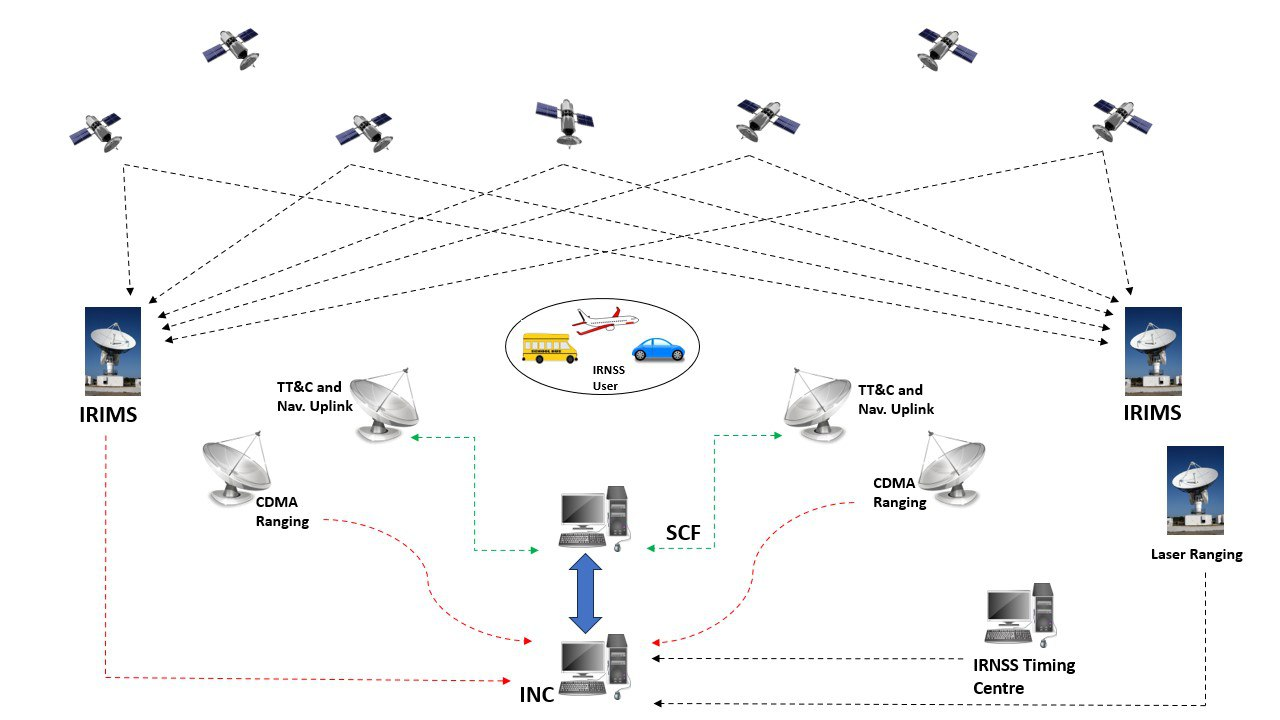
\includegraphics[width=\columnwidth]{figs/Architecture.jpg}
	\caption{NavIC Architecture}
	\label{figs:archfig}
	\end{figure}

\subsection{Space segment}
Space segment consists of a constellation of $7$ satellites. Three satellites of the constellation are placed in geostationary orbit, at $32.5^{\circ}$E, $83^{\circ}$E and $129.5^{\circ}$E respectively, and four satellites are placed in inclined geosynchronous orbit with equatorial crossing of $55^{\circ}$E and $111.75^{\circ}$E respectively, with inclination of $29^{\circ}$ (two satellites in each plane).

\subsection{Ground segment}
Ground segment takes care of operation and maintenance of the constellation. It consists of 
\begin{enumerate}
	\item ISRO Navigation Centre
	\item IRNSS Spacecraft Control Facility
	\item IRNSS Range and Integrity Monitoring Stations
	\item IRNSS Network Timing Centre
	\item IRNSS CDMA Ranging Stations
	\item Laser Ranging Stations
	\item Data Communication Network
\end{enumerate}

\subsection{User segment}
User segment consists of 
\begin{enumerate}
	\item A single frequency receiver having capability to receive SPS signal at either L1, L5 or S band frequency
	\item A multi-frequency receiver having capability to receive SPS signal at combination of L1, L5 and S band frequencies
	\item A multi-constellation receiver compatible with NavIC and other GNSS signals.
\end{enumerate}
\noindent The Figure\ref{figs:bandsfig} above specifies the radio frequency interface between space and user segments.

	\begin{figure}[!ht]
	\centering
	%\subimport{table/}{table1.tex}
	\tikzset{every picture/.style={line width=0.75pt}} %set default line width to 0.75pt        
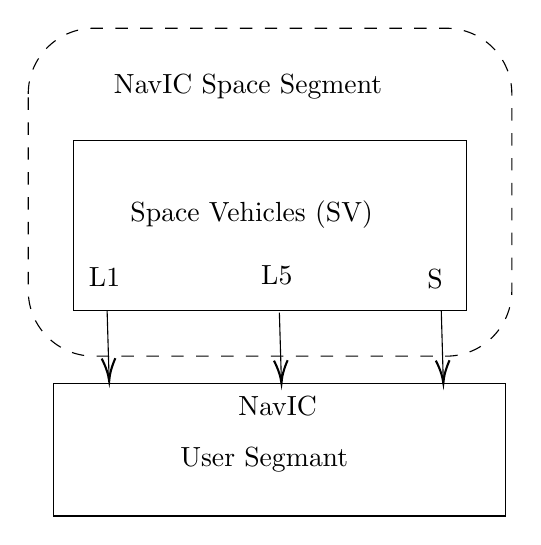
\begin{tikzpicture}[x=0.75pt,y=0.75pt,yscale=-1,xscale=1]
%uncomment if require: \path (0,406); %set diagram left start at 0, and has height of 406

%Shape: Rectangle [id:dp7411978076301706] 
\draw   (254,164) -- (443,164) -- (443,246) -- (254,246) -- cycle ;
%Straight Lines [id:da11098118487919195] 
\draw    (270,246) -- (270.94,278) ;
\draw [shift={(271,280)}, rotate = 268.32] [color={rgb, 255:red, 0; green, 0; blue, 0 }  ][line width=0.75]    (10.93,-3.29) .. controls (6.95,-1.4) and (3.31,-0.3) .. (0,0) .. controls (3.31,0.3) and (6.95,1.4) .. (10.93,3.29)   ;
%Shape: Rectangle [id:dp29610782491063636] 
\draw   (244,281) -- (462,281) -- (462,345) -- (244,345) -- cycle ;
%Straight Lines [id:da1330694648577655] 
\draw    (353,247) -- (353.94,279) ;
\draw [shift={(354,281)}, rotate = 268.32] [color={rgb, 255:red, 0; green, 0; blue, 0 }  ][line width=0.75]    (10.93,-3.29) .. controls (6.95,-1.4) and (3.31,-0.3) .. (0,0) .. controls (3.31,0.3) and (6.95,1.4) .. (10.93,3.29)   ;
%Straight Lines [id:da06268750746850027] 
\draw    (431,246) -- (431.94,279) ;
\draw [shift={(432,281)}, rotate = 268.36] [color={rgb, 255:red, 0; green, 0; blue, 0 }  ][line width=0.75]    (10.93,-3.29) .. controls (6.95,-1.4) and (3.31,-0.3) .. (0,0) .. controls (3.31,0.3) and (6.95,1.4) .. (10.93,3.29)   ;
%Rounded Rect [id:dp5981425610685245] 
\draw  [dash pattern={on 4.5pt off 4.5pt}] (232,141.6) .. controls (232,124.15) and (246.15,110) .. (263.6,110) -- (433.4,110) .. controls (450.85,110) and (465,124.15) .. (465,141.6) -- (465,236.4) .. controls (465,253.85) and (450.85,268) .. (433.4,268) -- (263.6,268) .. controls (246.15,268) and (232,253.85) .. (232,236.4) -- cycle ;

% Text Node
\draw (272,131) node [anchor=north west][inner sep=0.75pt]   [align=left] {NavIC Space Segment};
% Text Node
\draw (280,192) node [anchor=north west][inner sep=0.75pt]   [align=left] {Space Vehicles (SV)};
% Text Node
\draw (260,224) node [anchor=north west][inner sep=0.75pt]   [align=left] {L1};
% Text Node
\draw (343,223) node [anchor=north west][inner sep=0.75pt]   [align=left] {L5};
% Text Node
\draw (423,225) node [anchor=north west][inner sep=0.75pt]   [align=left] {S};
% Text Node
\draw (332,286) node [anchor=north west][inner sep=0.75pt]   [align=left] {NavIC};
% Text Node
\draw (304,311) node [anchor=north west][inner sep=0.75pt]   [align=left] {User Segmant};

\end{tikzpicture}

	\caption{the NavIC bands segment blocks}
	\label{figs:bandsfig}
	\end{figure}

\section{NavIC Services}
The NavIC provides basically two types of services:
	\begin{enumerate}
	\item Standard Positioning Service (SPS)
	\item Restricted Service (RS)
	\end{enumerate}
Both SPS and RS signals contain ranging codes that allow receivers to compute their travelling time from satellite to receiver, along with navigation data, in order to know the satellite’s position at any time. 
\subsection{Standard Positioning Service (SPS)}
	It is available to all civilian users free of charge and provides positioning, navigation, and timing information with a moderate level of accuracy. The SPS signals in NavIC primarily operate in the L5 and S frequency bands.
\subsection{Restricted Service (RS)}
The RS is intended for authorized users and offers enhanced accuracy, integrity, and availability compared to the SPS signals. The RS signals in NavIC operate in both the L5 and S bands and broadcast through a phased array antenna to keep required coverage and signal strength. 
%\end{document}

\chapter{Transmitter}
The NavIC transmitter is simulated to send baseband signal to the channel as shown in Fig \ref{fig:trans_flow}. 

\begin{figure}[ht]
\centering
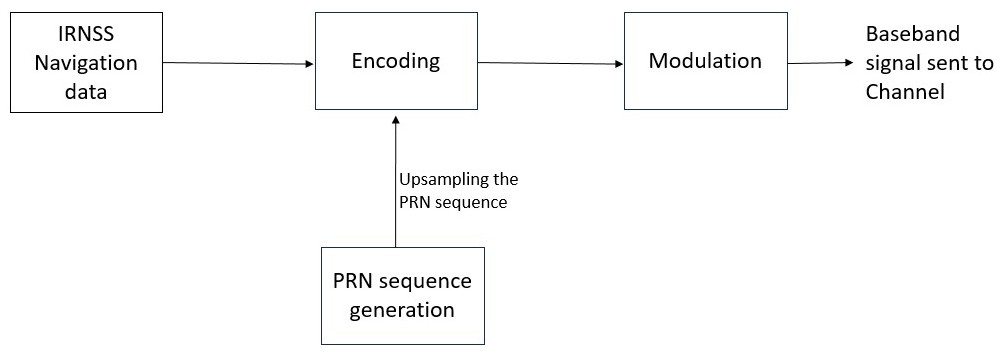
\includegraphics[width=1\columnwidth]{figs/trans_flow.jpg}
\centering
\captionsetup{justification=centering}
\caption{Transmitter Block diagram}
\label{fig:trans_flow}
\end{figure}

\section{IRNSS Navigation data}
Navigation data in satellite communication refers to the crucial information transmitted between satellites and ground-based receivers to facilitate accurate positioning and navigation. It includes data related to satellite orbits, precise timing, and other parameters necessary for determining the satellite's position relative to the Earth's surface.
\section{Frame structure}
NavIC master frame consists of $2400$ symbols, divided into $4$ subframes. Each subframe is $600$ symbols long. Each subframe has $16$ bit Sync word followed by $584$ bits of interleaved data. Subframes $1$ and $2$ transmit fixed primar navigation parameters. Subframe $3$ and $4$ transmit secondary navigation parameters in the form of messages. The master frame structure is shown in figure \ref{fig:master_frame}. 

\begin{figure}[ht]
\centering
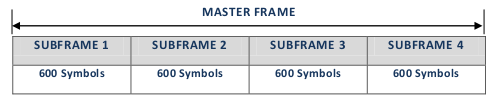
\includegraphics[width=0.8\columnwidth]{figs/master_frame.png}
\centering
\captionsetup{justification=centering}
\caption{Master Frame Structure}
\label{fig:master_frame}
\end{figure}

\noindent Each subframe is $292$ bits long without FEC encoding and sync word. It starts with TLM word of 8 bits and ends with $24$ bit Cyclic Redundancy Check(CRC) followed by $6$ tail bits. In subframes $1$ and $2$ navigation data is alloted with $232$ bits, starting from bit $31$. In subframe $3$ and $4$, $220$ bits are alloted starting from bit $37$. The typical structure of the subframes are shown in figure \ref{fig:frame_1_2} and figure \ref{fig:frame_3_4} respectively.

\begin{figure}[ht]
\centering
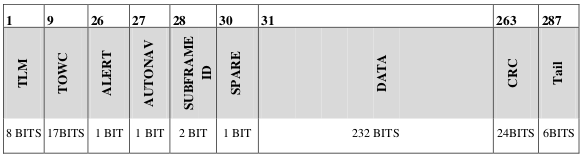
\includegraphics[width=0.8\columnwidth]{figs/1_2.png}
\centering
\captionsetup{justification=centering}
\caption{Structure of subframe 1 and 2}
\label{fig:frame_1_2}
\end{figure}

\begin{figure}[ht]
\centering
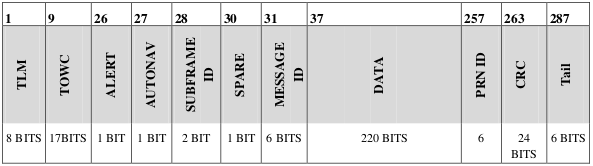
\includegraphics[width=0.8\columnwidth]{figs/3_4.png}
\centering
\captionsetup{justification=centering}
\caption{Structure of subframe 3 and 4}
\label{fig:frame_3_4}
\end{figure}

\section{Encoding}
\subsection{PRN codes for SPS}
PRN Codes selected for Standard Positioning System are similar to GPS C/A Gold codes. The length of each code is $1023$ chips. The code is chipped at $1.023$ Mcps.

\noindent For SPS code generation, the two polynomials G1 and G2 are as defined below:
\begin{align}
G1 &: X^{10}+X^{3} + 1\\
G2 &: X^{10}+X^9+X^8+X^6+X^3+X^2+1
\end{align}
Polynomial G1 and G2 are similar to the ones used by GPS C/A signal. The G1 and G2 generators are realized by using $10$ bits Maximum Length Feedback Shift Registers(MLFSR). The initial state of G2 provides the chip delay. The G1 register is initialized with all bits as $1$. G1 and G2 are XOR'ed for the generation of the final $1023$ chip long PRN sequence. The SPS PRN code generator is shown in figure \ref{figure:codeGen}.

\begin{figure}[!ht]
	\centering
	\tikzset{every picture/.style={line width=0.75pt}} %set default line width to 0.75pt        

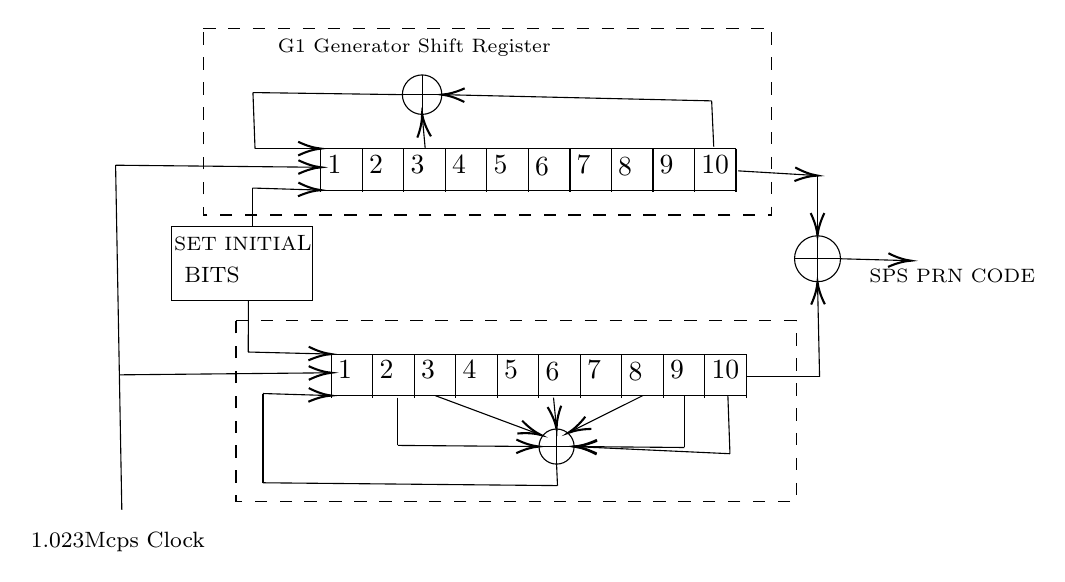
\begin{tikzpicture}[x=0.75pt,y=0.75pt,yscale=-1,xscale=1]
%uncomment if require: \path (0,300); %set diagram left start at 0, and has height of 300

%Shape: Grid [id:dp4759069175630535] 
\draw  [draw opacity=0] (187,78.28) -- (387.09,78.28) -- (387.09,99.28) -- (187,99.28) -- cycle ; \draw   (187,78.28) -- (187,99.28)(207,78.28) -- (207,99.28)(227,78.28) -- (227,99.28)(247,78.28) -- (247,99.28)(267,78.28) -- (267,99.28)(287,78.28) -- (287,99.28)(307,78.28) -- (307,99.28)(327,78.28) -- (327,99.28)(347,78.28) -- (347,99.28)(367,78.28) -- (367,99.28)(387,78.28) -- (387,99.28) ; \draw   (187,78.28) -- (387.09,78.28)(187,98.28) -- (387.09,98.28) ; \draw    ;
%Straight Lines [id:da569456764054443] 
\draw    (88.09,86.28) -- (185.09,87.26) ;
\draw [shift={(187.09,87.28)}, rotate = 180.58] [color={rgb, 255:red, 0; green, 0; blue, 0 }  ][line width=0.75]    (10.93,-3.29) .. controls (6.95,-1.4) and (3.31,-0.3) .. (0,0) .. controls (3.31,0.3) and (6.95,1.4) .. (10.93,3.29)   ;
%Straight Lines [id:da10333590103804569] 
\draw    (155.27,78.28) -- (185,78.28) ;
\draw [shift={(187,78.28)}, rotate = 180] [color={rgb, 255:red, 0; green, 0; blue, 0 }  ][line width=0.75]    (10.93,-3.29) .. controls (6.95,-1.4) and (3.31,-0.3) .. (0,0) .. controls (3.31,0.3) and (6.95,1.4) .. (10.93,3.29)   ;
%Straight Lines [id:da24492265686656967] 
\draw    (154.09,97.28) -- (185,98.22) ;
\draw [shift={(187,98.28)}, rotate = 181.74] [color={rgb, 255:red, 0; green, 0; blue, 0 }  ][line width=0.75]    (10.93,-3.29) .. controls (6.95,-1.4) and (3.31,-0.3) .. (0,0) .. controls (3.31,0.3) and (6.95,1.4) .. (10.93,3.29)   ;
%Straight Lines [id:da7870160753562048] 
\draw    (88.09,86.28) -- (91.09,252.28) ;
%Shape: Grid [id:dp16213094638707903] 
\draw  [draw opacity=0] (192,177.28) -- (392.09,177.28) -- (392.09,198.28) -- (192,198.28) -- cycle ; \draw   (192,177.28) -- (192,198.28)(212,177.28) -- (212,198.28)(232,177.28) -- (232,198.28)(252,177.28) -- (252,198.28)(272,177.28) -- (272,198.28)(292,177.28) -- (292,198.28)(312,177.28) -- (312,198.28)(332,177.28) -- (332,198.28)(352,177.28) -- (352,198.28)(372,177.28) -- (372,198.28)(392,177.28) -- (392,198.28) ; \draw   (192,177.28) -- (392.09,177.28)(192,197.28) -- (392.09,197.28) ; \draw    ;
%Straight Lines [id:da7354388024747429] 
\draw    (90.09,187.28) -- (190.09,186.3) ;
\draw [shift={(192.09,186.28)}, rotate = 179.44] [color={rgb, 255:red, 0; green, 0; blue, 0 }  ][line width=0.75]    (10.93,-3.29) .. controls (6.95,-1.4) and (3.31,-0.3) .. (0,0) .. controls (3.31,0.3) and (6.95,1.4) .. (10.93,3.29)   ;
%Straight Lines [id:da7447494470460669] 
\draw    (152,176.28) -- (190,177.23) ;
\draw [shift={(192,177.28)}, rotate = 181.43] [color={rgb, 255:red, 0; green, 0; blue, 0 }  ][line width=0.75]    (10.93,-3.29) .. controls (6.95,-1.4) and (3.31,-0.3) .. (0,0) .. controls (3.31,0.3) and (6.95,1.4) .. (10.93,3.29)   ;
%Straight Lines [id:da031744246724348946] 
\draw    (159.09,196.28) -- (190,197.22) ;
\draw [shift={(192,197.28)}, rotate = 181.74] [color={rgb, 255:red, 0; green, 0; blue, 0 }  ][line width=0.75]    (10.93,-3.29) .. controls (6.95,-1.4) and (3.31,-0.3) .. (0,0) .. controls (3.31,0.3) and (6.95,1.4) .. (10.93,3.29)   ;
%Shape: Rectangle [id:dp3444409778450146] 
\draw   (115.09,116) -- (183,116) -- (183,151.28) -- (115.09,151.28) -- cycle ;
%Straight Lines [id:da8394882855126624] 
\draw    (154.09,97.28) -- (154.09,116.28) ;
%Straight Lines [id:da8844900237810436] 
\draw    (155.27,78.28) -- (154.27,51.28) ;
%Shape: Rectangle [id:dp4508883643682198] 
\draw  [dash pattern={on 4.5pt off 4.5pt}] (146.09,161.28) -- (416.09,161.28) -- (416.09,248.28) -- (146.09,248.28) -- cycle ;
%Shape: Circle [id:dp6333600485336248] 
\draw   (292.09,221.82) .. controls (292.09,217.15) and (295.88,213.37) .. (300.55,213.37) .. controls (305.21,213.37) and (309,217.15) .. (309,221.82) .. controls (309,226.49) and (305.21,230.28) .. (300.55,230.28) .. controls (295.88,230.28) and (292.09,226.49) .. (292.09,221.82) -- cycle ;
%Straight Lines [id:da565085930383092] 
\draw    (309,221.82) -- (292.09,221.82) ;
%Straight Lines [id:da42773099028752415] 
\draw    (300.55,213.37) -- (300.55,230.28) ;
%Straight Lines [id:da3290835690299596] 
\draw    (224.09,221.28) -- (290.09,221.81) ;
\draw [shift={(292.09,221.82)}, rotate = 180.46] [color={rgb, 255:red, 0; green, 0; blue, 0 }  ][line width=0.75]    (10.93,-3.29) .. controls (6.95,-1.4) and (3.31,-0.3) .. (0,0) .. controls (3.31,0.3) and (6.95,1.4) .. (10.93,3.29)   ;
%Straight Lines [id:da4691319269868135] 
\draw    (224.09,198.28) -- (224.09,221.28) ;
%Straight Lines [id:da5103290679671173] 
\draw    (242.09,197.28) -- (291.22,215.58) ;
\draw [shift={(293.09,216.28)}, rotate = 200.43] [color={rgb, 255:red, 0; green, 0; blue, 0 }  ][line width=0.75]    (10.93,-3.29) .. controls (6.95,-1.4) and (3.31,-0.3) .. (0,0) .. controls (3.31,0.3) and (6.95,1.4) .. (10.93,3.29)   ;
%Straight Lines [id:da0749725526206042] 
\draw    (299.09,198.28) -- (300.35,211.38) ;
\draw [shift={(300.55,213.37)}, rotate = 264.49] [color={rgb, 255:red, 0; green, 0; blue, 0 }  ][line width=0.75]    (10.93,-3.29) .. controls (6.95,-1.4) and (3.31,-0.3) .. (0,0) .. controls (3.31,0.3) and (6.95,1.4) .. (10.93,3.29)   ;
%Straight Lines [id:da3968214865752646] 
\draw    (342.09,197.28) -- (307.88,214.38) ;
\draw [shift={(306.09,215.28)}, rotate = 333.43] [color={rgb, 255:red, 0; green, 0; blue, 0 }  ][line width=0.75]    (10.93,-3.29) .. controls (6.95,-1.4) and (3.31,-0.3) .. (0,0) .. controls (3.31,0.3) and (6.95,1.4) .. (10.93,3.29)   ;
%Straight Lines [id:da8862982187324178] 
\draw    (362.09,222.28) -- (311,221.84) ;
\draw [shift={(309,221.82)}, rotate = 0.49] [color={rgb, 255:red, 0; green, 0; blue, 0 }  ][line width=0.75]    (10.93,-3.29) .. controls (6.95,-1.4) and (3.31,-0.3) .. (0,0) .. controls (3.31,0.3) and (6.95,1.4) .. (10.93,3.29)   ;
%Straight Lines [id:da371299798629132] 
\draw    (362.09,197.28) -- (362.09,222.28) ;
%Straight Lines [id:da021817449039569503] 
\draw    (384.09,225.28) -- (311,221.92) ;
\draw [shift={(309,221.82)}, rotate = 2.63] [color={rgb, 255:red, 0; green, 0; blue, 0 }  ][line width=0.75]    (10.93,-3.29) .. controls (6.95,-1.4) and (3.31,-0.3) .. (0,0) .. controls (3.31,0.3) and (6.95,1.4) .. (10.93,3.29)   ;
%Straight Lines [id:da9332681631618418] 
\draw    (383.09,197.28) -- (384.09,225.28) ;
%Straight Lines [id:da3829411398928415] 
\draw    (159.09,196.28) -- (159.09,239.28) ;
%Straight Lines [id:da10453610903709909] 
\draw    (159.09,239.28) -- (301,240.64) ;
%Straight Lines [id:da0007774149610855208] 
\draw    (301,240.64) -- (300.55,230.28) ;
%Straight Lines [id:da6330583818759461] 
\draw    (152.09,151.28) -- (152,176.28) ;
%Straight Lines [id:da00902543002259093] 
\draw    (154.27,51.28) -- (226.27,52.28) ;
%Shape: Circle [id:dp535536355916993] 
\draw   (226.27,52.28) .. controls (226.27,47.03) and (230.53,42.78) .. (235.77,42.78) .. controls (241.02,42.78) and (245.27,47.03) .. (245.27,52.28) .. controls (245.27,57.53) and (241.02,61.78) .. (235.77,61.78) .. controls (230.53,61.78) and (226.27,57.53) .. (226.27,52.28) -- cycle ;
%Straight Lines [id:da7475335834022037] 
\draw    (388,89) -- (424.28,91.16) ;
\draw [shift={(426.27,91.28)}, rotate = 183.41] [color={rgb, 255:red, 0; green, 0; blue, 0 }  ][line width=0.75]    (10.93,-3.29) .. controls (6.95,-1.4) and (3.31,-0.3) .. (0,0) .. controls (3.31,0.3) and (6.95,1.4) .. (10.93,3.29)   ;
%Shape: Rectangle [id:dp33628232360328436] 
\draw  [dash pattern={on 4.5pt off 4.5pt}] (130.27,20.28) -- (404.27,20.28) -- (404.27,110.28) -- (130.27,110.28) -- cycle ;
%Straight Lines [id:da4528593286074343] 
\draw    (226.27,52.28) -- (245.27,52.28) ;
%Straight Lines [id:da4935198786917454] 
\draw    (235.77,42.78) -- (235.77,61.78) ;
%Straight Lines [id:da006409026658961592] 
\draw    (237.27,78.28) -- (235.95,63.77) ;
\draw [shift={(235.77,61.78)}, rotate = 84.81] [color={rgb, 255:red, 0; green, 0; blue, 0 }  ][line width=0.75]    (10.93,-3.29) .. controls (6.95,-1.4) and (3.31,-0.3) .. (0,0) .. controls (3.31,0.3) and (6.95,1.4) .. (10.93,3.29)   ;
%Straight Lines [id:da7723649958376586] 
\draw    (375.27,55.28) -- (247.27,52.32) ;
\draw [shift={(245.27,52.28)}, rotate = 1.32] [color={rgb, 255:red, 0; green, 0; blue, 0 }  ][line width=0.75]    (10.93,-3.29) .. controls (6.95,-1.4) and (3.31,-0.3) .. (0,0) .. controls (3.31,0.3) and (6.95,1.4) .. (10.93,3.29)   ;
%Straight Lines [id:da81665598367533] 
\draw    (375.27,55.28) -- (376.27,77.28) ;
%Straight Lines [id:da7592139843126284] 
\draw    (426.27,91.28) -- (426.27,118.28) ;
\draw [shift={(426.27,120.28)}, rotate = 270] [color={rgb, 255:red, 0; green, 0; blue, 0 }  ][line width=0.75]    (10.93,-3.29) .. controls (6.95,-1.4) and (3.31,-0.3) .. (0,0) .. controls (3.31,0.3) and (6.95,1.4) .. (10.93,3.29)   ;
%Shape: Circle [id:dp3559277528699165] 
\draw   (415.2,131.35) .. controls (415.2,125.23) and (420.16,120.28) .. (426.27,120.28) .. controls (432.39,120.28) and (437.34,125.23) .. (437.34,131.35) .. controls (437.34,137.46) and (432.39,142.41) .. (426.27,142.41) .. controls (420.16,142.41) and (415.2,137.46) .. (415.2,131.35) -- cycle ;
%Straight Lines [id:da5291717879618754] 
\draw    (427.27,188.28) -- (426.32,144.41) ;
\draw [shift={(426.27,142.41)}, rotate = 88.75] [color={rgb, 255:red, 0; green, 0; blue, 0 }  ][line width=0.75]    (10.93,-3.29) .. controls (6.95,-1.4) and (3.31,-0.3) .. (0,0) .. controls (3.31,0.3) and (6.95,1.4) .. (10.93,3.29)   ;
%Straight Lines [id:da5415214890722322] 
\draw    (392.27,188.28) -- (427.27,188.28) ;
%Straight Lines [id:da6601024458299296] 
\draw    (415.2,131.35) -- (437.34,131.35) ;
%Straight Lines [id:da455975979596007] 
\draw    (426.27,120.28) -- (426.27,142.41) ;
%Straight Lines [id:da36345454664351773] 
\draw    (437.34,131.35) -- (469.27,132.22) ;
\draw [shift={(471.27,132.28)}, rotate = 181.57] [color={rgb, 255:red, 0; green, 0; blue, 0 }  ][line width=0.75]    (10.93,-3.29) .. controls (6.95,-1.4) and (3.31,-0.3) .. (0,0) .. controls (3.31,0.3) and (6.95,1.4) .. (10.93,3.29)   ;

% Text Node
\draw (189,80.28) node [anchor=north west][inner sep=0.75pt]   [align=left] {1};
% Text Node
\draw (209,80.28) node [anchor=north west][inner sep=0.75pt]   [align=left] {2};
% Text Node
\draw (229,80.28) node [anchor=north west][inner sep=0.75pt]   [align=left] {3};
% Text Node
\draw (249,80.28) node [anchor=north west][inner sep=0.75pt]   [align=left] {4};
% Text Node
\draw (269,80.28) node [anchor=north west][inner sep=0.75pt]   [align=left] {5};
% Text Node
\draw (289,81.28) node [anchor=north west][inner sep=0.75pt]   [align=left] {6};
% Text Node
\draw (309,80.28) node [anchor=north west][inner sep=0.75pt]   [align=left] {7};
% Text Node
\draw (329,81.28) node [anchor=north west][inner sep=0.75pt]   [align=left] {8};
% Text Node
\draw (349,80.28) node [anchor=north west][inner sep=0.75pt]   [align=left] {9};
% Text Node
\draw (369,80.28) node [anchor=north west][inner sep=0.75pt]   [align=left] {10};
% Text Node
\draw (46,262) node [anchor=north west][inner sep=0.75pt]  [font=\footnotesize] [align=left] {1.023Mcps Clock};
% Text Node
\draw (194,179.28) node [anchor=north west][inner sep=0.75pt]   [align=left] {1};
% Text Node
\draw (214,179.28) node [anchor=north west][inner sep=0.75pt]   [align=left] {2};
% Text Node
\draw (234,179.28) node [anchor=north west][inner sep=0.75pt]   [align=left] {3};
% Text Node
\draw (254,179.28) node [anchor=north west][inner sep=0.75pt]   [align=left] {4};
% Text Node
\draw (274,179.28) node [anchor=north west][inner sep=0.75pt]   [align=left] {5};
% Text Node
\draw (294,180.28) node [anchor=north west][inner sep=0.75pt]   [align=left] {6};
% Text Node
\draw (314,179.28) node [anchor=north west][inner sep=0.75pt]   [align=left] {7};
% Text Node
\draw (354,179.28) node [anchor=north west][inner sep=0.75pt]   [align=left] {9};
% Text Node
\draw (374,179.28) node [anchor=north west][inner sep=0.75pt]   [align=left] {10};
% Text Node
\draw (334,180.28) node [anchor=north west][inner sep=0.75pt]   [align=left] {8};
% Text Node
\draw (115,119) node [anchor=north west][inner sep=0.75pt]   [align=left] {{\scriptsize SET INITIA}{\footnotesize L}};
% Text Node
\draw (120,134) node [anchor=north west][inner sep=0.75pt]   [align=left] {{\footnotesize BITS}};
% Text Node
\draw (450,135) node [anchor=north west][inner sep=0.75pt]   [align=left] {{\scriptsize SPS PRN CODE}};
% Text Node
\draw (165,24) node [anchor=north west][inner sep=0.75pt]   [align=left] {{\scriptsize G1 Generator Shift Register}};


\end{tikzpicture}

	\caption{SPS PRN Code Generator}
	\label{figure:codeGen}
\end{figure}

\noindent The satellites that are used in the current code implementation are with PRN ids - $1,3,5$ and $7$. The initial condition of G2 register in L5 and S bands for the given PRN ids is given in table \ref{table:sps_codes}.

\begin{table}[h]
%\centering
%%%%%%%%%%%%%%%%%%%%%%%%%%%%%%%%%%%%%%%%%%%%%%%%%%%%%%%%%%%%%%%%%%%%%%
%%                                                                  %%
%%  This is the header of a LaTeX2e file exported from Gnumeric.    %%
%%                                                                  %%
%%  This file can be compiled as it stands or included in another   %%
%%  LaTeX document. The table is based on the longtable package so  %%
%%  the longtable options (headers, footers...) can be set in the   %%
%%  preamble section below (see PRAMBLE).                           %%
%%                                                                  %%
%%  To include the file in another, the following two lines must be %%
%%  in the including file:                                          %%
%%        \def\inputGnumericTable{}                                 %%
%%  at the beginning of the file and:                               %%
%%        \input{name-of-this-file.tex}                             %%
%%  where the table is to be placed. Note also that the including   %%
%%  file must use the following packages for the table to be        %%
%%  rendered correctly:                                             %%
%%    \usepackage[latin1]{inputenc}                                 %%
%%    \usepackage{color}                                            %%
%%    \usepackage{array}                                            %%
%%    \usepackage{longtable}                                        %%
%%    \usepackage{calc}                                             %%
%%    \usepackage{multirow}                                         %%
%%    \usepackage{hhline}                                           %%
%%    \usepackage{ifthen}                                           %%
%%  optionally (for landscape tables embedded in another document): %%
%%    \usepackage{lscape}                                           %%
%%                                                                  %%
%%%%%%%%%%%%%%%%%%%%%%%%%%%%%%%%%%%%%%%%%%%%%%%%%%%%%%%%%%%%%%%%%%%%%%



%%  This section checks if we are begin input into another file or  %%
%%  the file will be compiled alone. First use a macro taken from   %%
%%  the TeXbook ex 7.7 (suggestion of Han-Wen Nienhuys).            %%
\def\ifundefined#1{\expandafter\ifx\csname#1\endcsname\relax}


%%  Check for the \def token for inputed files. If it is not        %%
%%  defined, the file will be processed as a standalone and the     %%
%%  preamble will be used.                                          %%
\ifundefined{inputGnumericTable}

%%  We must be able to close or not the document at the end.        %%
	\def\gnumericTableEnd{\end{document}}


%%%%%%%%%%%%%%%%%%%%%%%%%%%%%%%%%%%%%%%%%%%%%%%%%%%%%%%%%%%%%%%%%%%%%%
%%                                                                  %%
%%  This is the PREAMBLE. Change these values to get the right      %%
%%  paper size and other niceties.                                  %%
%%                                                                  %%
%%%%%%%%%%%%%%%%%%%%%%%%%%%%%%%%%%%%%%%%%%%%%%%%%%%%%%%%%%%%%%%%%%%%%%

	\documentclass[12pt%
			  %,landscape%
                    ]{report}
       \usepackage[latin1]{inputenc}
       \usepackage{fullpage}
       \usepackage{color}
       \usepackage{array}
       \usepackage{longtable}
       \usepackage{calc}
       \usepackage{multirow}
       \usepackage{hhline}
       \usepackage{ifthen}

	\begin{document}


%%  End of the preamble for the standalone. The next section is for %%
%%  documents which are included into other LaTeX2e files.          %%
\else

%%  We are not a stand alone document. For a regular table, we will %%
%%  have no preamble and only define the closing to mean nothing.   %%
    \def\gnumericTableEnd{}

%%  If we want landscape mode in an embedded document, comment out  %%
%%  the line above and uncomment the two below. The table will      %%
%%  begin on a new page and run in landscape mode.                  %%
%       \def\gnumericTableEnd{\end{landscape}}
%       \begin{landscape}


%%  End of the else clause for this file being \input.              %%
\fi

%%%%%%%%%%%%%%%%%%%%%%%%%%%%%%%%%%%%%%%%%%%%%%%%%%%%%%%%%%%%%%%%%%%%%%
%%                                                                  %%
%%  The rest is the gnumeric table, except for the closing          %%
%%  statement. Changes below will alter the table's appearance.     %%
%%                                                                  %%
%%%%%%%%%%%%%%%%%%%%%%%%%%%%%%%%%%%%%%%%%%%%%%%%%%%%%%%%%%%%%%%%%%%%%%

\providecommand{\gnumericmathit}[1]{#1} 
%%  Uncomment the next line if you would like your numbers to be in %%
%%  italics if they are italizised in the gnumeric table.           %%
%\renewcommand{\gnumericmathit}[1]{\mathit{#1}}
\providecommand{\gnumericPB}[1]%
{\let\gnumericTemp=\\#1\let\\=\gnumericTemp\hspace{0pt}}
 \ifundefined{gnumericTableWidthDefined}
        \newlength{\gnumericTableWidth}
        \newlength{\gnumericTableWidthComplete}
        \newlength{\gnumericMultiRowLength}
        \global\def\gnumericTableWidthDefined{}
 \fi
%% The following setting protects this code from babel shorthands.  %%
 \ifthenelse{\isundefined{\languageshorthands}}{}{\languageshorthands{english}}
%%  The default table format retains the relative column widths of  %%
%%  gnumeric. They can easily be changed to c, r or l. In that case %%
%%  you may want to comment out the next line and uncomment the one %%
%%  thereafter                                                      %%
\providecommand\gnumbox{\makebox[0pt]}
%%\providecommand\gnumbox[1][]{\makebox}

%% to adjust positions in multirow situations                       %%
\setlength{\bigstrutjot}{\jot}
\setlength{\extrarowheight}{\doublerulesep}

%%  The \setlongtables command keeps column widths the same across  %%
%%  pages. Simply comment out next line for varying column widths.  %%
\setlongtables

\setlength\gnumericTableWidth{%
	5pt+%
	30pt+%
	30pt+%
0pt}
\def\gumericNumCols{3}
\setlength\gnumericTableWidthComplete{\gnumericTableWidth+%
         \tabcolsep*\gumericNumCols*3+\arrayrulewidth*\gumericNumCols}
\ifthenelse{\lengthtest{\gnumericTableWidthComplete > \linewidth}}%
         {\def\gnumericScale{\ratio{\linewidth-%
                        \tabcolsep*\gumericNumCols*3-%
                        \arrayrulewidth*\gumericNumCols}%
{\gnumericTableWidth}}}%
{\def\gnumericScale{1}}

%%%%%%%%%%%%%%%%%%%%%%%%%%%%%%%%%%%%%%%%%%%%%%%%%%%%%%%%%%%%%%%%%%%%%%
%%                                                                  %%
%% The following are the widths of the various columns. We are      %%
%% defining them here because then they are easier to change.       %%
%% Depending on the cell formats we may use them more than once.    %%
%%                                                                  %%
%%%%%%%%%%%%%%%%%%%%%%%%%%%%%%%%%%%%%%%%%%%%%%%%%%%%%%%%%%%%%%%%%%%%%%

\ifthenelse{\isundefined{\gnumericColA}}{\newlength{\gnumericColA}}{}\settowidth{\gnumericColA}{\begin{tabular}{@{}p{30pt*\gnumericScale}@{}}x\end{tabular}}
\ifthenelse{\isundefined{\gnumericColB}}{\newlength{\gnumericColB}}{}\settowidth{\gnumericColB}{\begin{tabular}{@{}p{115pt*\gnumericScale}@{}}x\end{tabular}}
\ifthenelse{\isundefined{\gnumericColC}}{\newlength{\gnumericColC}}{}\settowidth{\gnumericColC}{\begin{tabular}{@{}p{115pt*\gnumericScale}@{}}x\end{tabular}}

\begin{longtable}[c]{%
	b{\gnumericColA}%
	b{\gnumericColB}%
	b{\gnumericColC}%
	}

%%%%%%%%%%%%%%%%%%%%%%%%%%%%%%%%%%%%%%%%%%%%%%%%%%%%%%%%%%%%%%%%%%%%%%
%%  The longtable options. (Caption, headers... see Goosens, p.124) %%
%	\caption{The Table Caption.}             \\	%
% \hline	% Across the top of the table.
%%  The rest of these options are table rows which are placed on    %%
%%  the first, last or every page. Use \multicolumn if you want.    %%

%%  Header for the first page.                                      %%
%	\multicolumn{2}{c}{The First Header} \\ \hline 
%	\multicolumn{1}{c}{colTag}	%Column 1
%	&\multicolumn{1}{c}{colTag}	\\ \hline %Last column
%	\endfirsthead

%%  The running header definition.                                  %%
%	\hline
%	\multicolumn{2}{l}{\ldots\small\slshape continued} \\ \hline
%	\multicolumn{1}{c}{colTag}	%Column 1
%	&\multicolumn{1}{c}{colTag}	\\ \hline %Last column
%	\endhead

%%  The running footer definition.                                  %%
%	\hline
%	\multicolumn{2}{r}{\small\slshape continued\ldots} \\
%	\endfoot

%%  The ending footer definition.                                   %%
%	\multicolumn{2}{c}{That's all folks} \\ \hline 
%	\endlastfoot
%%%%%%%%%%%%%%%%%%%%%%%%%%%%%%%%%%%%%%%%%%%%%%%%%%%%%%%%%%%%%%%%%%%%%%

\hhline{|-|-|-|}
	 \multicolumn{1}{|p{\gnumericColA}|}%
	{\gnumericPB{\raggedright}\gnumbox[l]{\textbf{PRN}}}
	&\multicolumn{1}{p{\gnumericColB}|}%
	{\gnumericPB{\raggedright}\gnumbox[l]{\hspace{1.2cm}\textbf{L5-SPS}}}
	&\multicolumn{1}{p{\gnumericColC}|}%
	{\gnumericPB{\raggedright}\gnumbox[l]{\hspace{1.4cm}\textbf{S-SPS}}}
\\
%\hhline{|-|-|-|}
	 \multicolumn{1}{|p{\gnumericColA}|}%
	{\gnumericPB{\raggedright}\gnumbox[l]{\hspace{0.25cm}\textbf{ID}}}
	&\multicolumn{1}{p{\gnumericColB}|}%
	{\gnumericPB{\raggedright}\gnumbox[l]{\textbf{G2 initial condition}}}
	&\multicolumn{1}{p{\gnumericColC}|}%
	{\gnumericPB{\raggedright}\gnumbox[l]{\textbf{G2 initial condition}}}
\\
\hhline{|---|}
	 \multicolumn{1}{|p{\gnumericColA}|}%
	{\gnumericPB{\raggedright}\gnumbox[l]{\hspace{0.5cm}1}}
	&\multicolumn{1}{p{\gnumericColB}|}%
	{\gnumericPB{\raggedright}\gnumbox[l]{\hspace{1cm}1110100111}}
	&\multicolumn{1}{p{\gnumericColC}|}%
	{\gnumericPB{\raggedright}\gnumbox[l]{\hspace{1cm}0011101111}}
\\
\hhline{|---|}
	 \multicolumn{1}{|p{\gnumericColA}|}%
	{\gnumericPB{\raggedright}\gnumbox[l]{\hspace{0.5cm}3}}
	&\multicolumn{1}{p{\gnumericColB}|}%
	{\gnumericPB{\raggedright}\gnumbox[l]{\hspace{1cm}1000110100}}
	&\multicolumn{1}{p{\gnumericColC}|}%
	{\gnumericPB{\raggedright}\gnumbox[l]{\hspace{1cm}1000110001}}
\\
\hhline{|---|}
	 \multicolumn{1}{|p{\gnumericColA}|}%
	{\gnumericPB{\raggedright}\gnumbox[l]{\hspace{0.5cm}5}}
	&\multicolumn{1}{p{\gnumericColB}|}%
	{\gnumericPB{\raggedright}\gnumbox[l]{\hspace{1cm}1110110000}}
	&\multicolumn{1}{p{\gnumericColC}|}%
	{\gnumericPB{\raggedright}\gnumbox[l]{\hspace{1cm}1010010001}}
\\
\hhline{|---|}
	 \multicolumn{1}{|p{\gnumericColA}|}%
	{\gnumericPB{\raggedright}\gnumbox[l]{\hspace{0.5cm}7}}
	&\multicolumn{1}{p{\gnumericColB}|}%
	{\gnumericPB{\raggedright}\gnumbox[l]{\hspace{1cm}0000010100}}
	&\multicolumn{1}{p{\gnumericColC}|}%
	{\gnumericPB{\raggedright}\gnumbox[l]{\hspace{1cm}0010001110}}
\\
\hhline{|---|}
\end{longtable}

\ifthenelse{\isundefined{\languageshorthands}}{}{\languageshorthands{\languagename}}
\gnumericTableEnd

\vspace{3mm}
\caption{Code phase assignment for SPS signals}
\label{table:sps_codes}
\end{table}

\subsection{FEC Encoding}
The Navigation data subframe of $292$ bits is convolution encoded with a rate of 1/2 and clocked at $50$ symbols per second. The coding scheme is given in figure \ref{fig:FEC}. Each subframe of $292$ bits, after encoding, results in $584$ symbols.

\begin{figure}[ht]
\centering
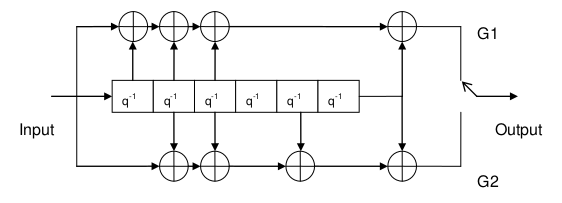
\includegraphics[width=\columnwidth]{figs/FEC.png}
\centering
\captionsetup{justification=centering}
\caption{FEC Encoding}
\label{fig:FEC}
\end{figure}

\subsection{Interleaving}
Any burst errors during the data transmission can be corrected by interleaving. In matrix interleaving, input symbols are filled into a matrix column wise and read at the output row wise. This will spread the burst error, if any, during the transmission. For SPS, data is filled into matrix of size $73$ by $8$($73$ columns, $8$ rows).
\subsection{Sync word and Tail bits}
Each subframe has a $16$ bit word synchronization pattern which is not encoded. Sync pattern is $EB90$ Hex. Tail bit consists of $6$ zero value bits enabling completion of FEC decoding of each subframe in the receiver.

\subsection{Cyclic Redundancy Check(CRC)}
The parity coding of data signal follows $24$Q polynomial for each subframe. $24$ bits of CRC parity will provide protection against burst as well as random errors with undetected error probability of $2^{-24}$ for all channel bit error probabilities $0.5$.
\begin{equation}
    g(X) = \sum_{i = 0}^{24}g_{i}X^i\;\; 
\end{equation}

    $g_{i}=1$; for $i = 0,1,3,4,5,6,7,10,11,14,17,18,23,24$ \\
          = 0 otherwise

\section{Modulation}

\subsection{Standard Positioning Service}
The SPS signal is BPSK(1) modulated on L5 and S bands. The navigation data at data rate of $50$ sps (1/2 rate FEC encoded) is modulo $2$ added to PRN code chipped at $1.023$ Mcps. The CDMA modulated code is upconverted by the L5 and S carriers at $1176.45$ MHz and $2492.028$ MHz respectively. However, this simulation does not carry out this upconversion.

\subsection{Baseband Modulation}
The carrier signal is modulated by BPSK(1), Data channel BOC(5,2), and Pilot Channel BOC(5,2). To have a constant envelop when passed through power amplifier, we add additional signal called interplex signal.

\subsubsection{Mathematical Equations}
\textbf{SPS Data Signal:}
\begin{equation}
	s_{sps}(t) = \sum_{i=-\infty}^{\infty} c_{sps}(\abs{i}_{L\_sps}) . d_{sps}(\sbrak{i}_{CD\_sps}) . rect_{T_{c,sps}}(t-iT_{c,sps})
\end{equation}
\textbf{RS BOC Pilot Signal:}
\begin{equation}
	s_{rs\_p}(t) = \sum_{i=-\infty}^{\infty} c_{rs\_p}(\abs{i}_{L\_rs\_p}) . rect_{Tc,rs\_p}(t-iT_{c,rs\_p}). sc_{rs\_p}(t,0)
\end{equation}
\textbf{RS BOC Signal:}
%\begin{equation}
\begin{multline}
	s_{rs\_d}(t) = \sum_{i=-\infty}^{\infty} c_{rs\_d}(\abs{i}_{L\_rs\_d}) . d_{rs\_d}(\sbrak{i}_{CD\_rs\_d}).  \\ 
	                       rect_{T_{c,rs\_d}}(t-iT_{c,rs\_d}). sc_{rs_d}(t,0)
\end{multline}
%\end{equation}
The sub-carrier is defined as:
\begin{equation}
	sc_x(t,\phi) = sgn\sbrak{sin(2 \pi f_{sc,x}t + \phi)}
\end{equation}

\noindent The IRNSS RS data and pilot BOC signals are sinBOC. Hence the subcarrier phase $\phi=0$.
The complex envelope of composite signal with Interplex signal (I(t)) is:
\begin{equation}
s(t) = \dfrac{1}{3} \sbrak{\sqrt{2} (s_{sps}(t) + s_{rs\_p}(t)) + j(2. s_{rs\_d}(t) - I(t))} 
\end{equation}

\noindent The Interplex signal $I(t)$ is generated to realize the constant envelope composite signal. The operation $\abs{i}_X$ gives the code chip index for any signal. Similarly $[i]_X$ gives data bit index for any signal.
Symbol definitions are given in below table \ref{table:symbdesc}.

\begin{table}[h]
%\centering
%%%%%%%%%%%%%%%%%%%%%%%%%%%%%%%%%%%%%%%%%%%%%%%%%%%%%%%%%%%%%%%%%%%%%%
%%                                                                  %%
%%  This is the header of a LaTeX2e file exported from Gnumeric.    %%
%%                                                                  %%
%%  This file can be compiled as it stands or included in another   %%
%%  LaTeX document. The table is based on the longtable package so  %%
%%  the longtable options (headers, footers...) can be set in the   %%
%%  preamble section below (see PRAMBLE).                           %%
%%                                                                  %%
%%  To include the file in another, the following two lines must be %%
%%  in the including file:                                          %%
%%        \def\inputGnumericTable{}                                 %%
%%  at the beginning of the file and:                               %%
%%        \input{name-of-this-file.tex}                             %%
%%  where the table is to be placed. Note also that the including   %%
%%  file must use the following packages for the table to be        %%
%%  rendered correctly:                                             %%
%%    \usepackage[latin1]{inputenc}                                 %%
%%    \usepackage{color}                                            %%
%%    \usepackage{array}                                            %%
%%    \usepackage{longtable}                                        %%
%    \usepackage{calc}                                             %%
%%    \usepackage{multirow}                                         %%
%%    \usepackage{hhline}                                           %%
%%    \usepackage{ifthen}                                           %%
%%  optionally (for landscape tables embedded in another document): %%
%%    \usepackage{lscape}                                           %%
%%                                                                  %%
%%%%%%%%%%%%%%%%%%%%%%%%%%%%%%%%%%%%%%%%%%%%%%%%%%%%%%%%%%%%%%%%%%%%%%



%%  This section checks if we are begin input into another file or  %%
%%  the file will be compiled alone. First use a macro taken from   %%
%%  the TeXbook ex 7.7 (suggestion of Han-Wen Nienhuys).            %%
\def\ifundefined#1{\expandafter\ifx\csname#1\endcsname\relax}


%%  Check for the \def token for inputed files. If it is not        %%
%%  defined, the file will be processed as a standalone and the     %%
%%  preamble will be used.                                          %%
\ifundefined{inputGnumericTable}

%%  We must be able to close or not the document at the end.        %%
	\def\gnumericTableEnd{\end{document}}


%%%%%%%%%%%%%%%%%%%%%%%%%%%%%%%%%%%%%%%%%%%%%%%%%%%%%%%%%%%%%%%%%%%%%%
%%                                                                  %%
%%  This is the PREAMBLE. Change these values to get the right      %%
%%  paper size and other niceties.                                  %%
%%                                                                  %%
%%%%%%%%%%%%%%%%%%%%%%%%%%%%%%%%%%%%%%%%%%%%%%%%%%%%%%%%%%%%%%%%%%%%%%

	\documentclass[12pt%
			  %,landscape%
                    ]{report}
       \usepackage[latin1]{inputenc}
       \usepackage{fullpage}
       \usepackage{color}
       \usepackage{array}
       \usepackage{longtable}
       \usepackage{calc}
       \usepackage{multirow}
       \usepackage{hhline}
       \usepackage{ifthen}

	\begin{document}


%%  End of the preamble for the standalone. The next section is for %%
%%  documents which are included into other LaTeX2e files.          %%
\else

%%  We are not a stand alone document. For a regular table, we will %%
%%  have no preamble and only define the closing to mean nothing.   %%
    \def\gnumericTableEnd{}

%%  If we want landscape mode in an embedded document, comment out  %%
%%  the line above and uncomment the two below. The table will      %%
%%  begin on a new page and run in landscape mode.                  %%
%       \def\gnumericTableEnd{\end{landscape}}
%       \begin{landscape}


%%  End of the else clause for this file being \input.              %%
\fi

%%%%%%%%%%%%%%%%%%%%%%%%%%%%%%%%%%%%%%%%%%%%%%%%%%%%%%%%%%%%%%%%%%%%%%
%%                                                                  %%
%%  The rest is the gnumeric table, except for the closing          %%
%%  statement. Changes below will alter the table's appearance.     %%
%%                                                                  %%
%%%%%%%%%%%%%%%%%%%%%%%%%%%%%%%%%%%%%%%%%%%%%%%%%%%%%%%%%%%%%%%%%%%%%%

\providecommand{\gnumericmathit}[1]{#1} 
%%  Uncomment the next line if you would like your numbers to be in %%
%%  italics if they are italizised in the gnumeric table.           %%
%\renewcommand{\gnumericmathit}[1]{\mathit{#1}}
\providecommand{\gnumericPB}[1]%
{\let\gnumericTemp=\\#1\let\\=\gnumericTemp\hspace{0pt}}
 \ifundefined{gnumericTableWidthDefined}
        \newlength{\gnumericTableWidth}
        \newlength{\gnumericTableWidthComplete}
        \newlength{\gnumericMultiRowLength}
        \global\def\gnumericTableWidthDefined{}
 \fi
%% The following setting protects this code from babel shorthands.  %%
 \ifthenelse{\isundefined{\languageshorthands}}{}{\languageshorthands{english}}
%%  The default table format retains the relative column widths of  %%
%%  gnumeric. They can easily be changed to c, r or l. In that case %%
%%  you may want to comment out the next line and uncomment the one %%
%%  thereafter                                                      %%
\providecommand\gnumbox{\makebox[0pt]}
%%\providecommand\gnumbox[1][]{\makebox}

%% to adjust positions in multirow situations                       %%
\setlength{\bigstrutjot}{\jot}
\setlength{\extrarowheight}{\doublerulesep}

%%  The \setlongtables command keeps column widths the same across  %%
%%  pages. Simply comment out next line for varying column widths.  %%
\setlongtables

\setlength\gnumericTableWidth{%
	80pt+%
	180pt+%
0pt}
\def\gumericNumCols{2}
\setlength\gnumericTableWidthComplete{\gnumericTableWidth+%
         \tabcolsep*\gumericNumCols*2+\arrayrulewidth*\gumericNumCols}
\ifthenelse{\lengthtest{\gnumericTableWidthComplete > \linewidth}}%
         {\def\gnumericScale{\ratio{\linewidth-%
                        \tabcolsep*\gumericNumCols*2-%
                        \arrayrulewidth*\gumericNumCols}%
{\gnumericTableWidth}}}%
{\def\gnumericScale{1}}

%%%%%%%%%%%%%%%%%%%%%%%%%%%%%%%%%%%%%%%%%%%%%%%%%%%%%%%%%%%%%%%%%%%%%%
%%                                                                  %%
%% The following are the widths of the various columns. We are      %%
%% defining them here because then they are easier to change.       %%
%% Depending on the cell formats we may use them more than once.    %%
%%                                                                  %%
%%%%%%%%%%%%%%%%%%%%%%%%%%%%%%%%%%%%%%%%%%%%%%%%%%%%%%%%%%%%%%%%%%%%%%

\ifthenelse{\isundefined{\gnumericColA}}{\newlength{\gnumericColA}}{}\settowidth{\gnumericColA}{\begin{tabular}{@{}p{80pt*\gnumericScale}@{}}x\end{tabular}}
\ifthenelse{\isundefined{\gnumericColB}}{\newlength{\gnumericColB}}{}\settowidth{\gnumericColB}{\begin{tabular}{@{}p{180pt*\gnumericScale}@{}}x\end{tabular}}

\begin{longtable}[c]{%
	b{\gnumericColA}%
	b{\gnumericColB}%
	}

%%%%%%%%%%%%%%%%%%%%%%%%%%%%%%%%%%%%%%%%%%%%%%%%%%%%%%%%%%%%%%%%%%%%%%
%%  The longtable options. (Caption, headers... see Goosens, p.124) %%
%	\caption{The Table Caption.}             \\	%
% \hline	% Across the top of the table.
%%  The rest of these options are table rows which are placed on    %%
%%  the first, last or every page. Use \multicolumn if you want.    %%

%%  Header for the first page.                                      %%
%	\multicolumn{2}{c}{The First Header} \\ \hline 
%	\multicolumn{1}{c}{colTag}	%Column 1
%	&\multicolumn{1}{c}{colTag}	\\ \hline %Last column
%	\endfirsthead

%%  The running header definition.                                  %%
%	\hline
%	\multicolumn{2}{l}{\ldots\small\slshape continued} \\ \hline
%	\multicolumn{1}{c}{colTag}	%Column 1
%	&\multicolumn{1}{c}{colTag}	\\ \hline %Last column
%	\endhead

%%  The running footer definition.                                  %%
%	\hline
%	\multicolumn{2}{r}{\small\slshape continued\ldots} \\
%	\endfoot

%%  The ending footer definition.                                   %%
%	\multicolumn{2}{c}{That's all folks} \\ \hline 
%	\endlastfoot
%%%%%%%%%%%%%%%%%%%%%%%%%%%%%%%%%%%%%%%%%%%%%%%%%%%%%%%%%%%%%%%%%%%%%%

\hhline{|-|-}
	 \multicolumn{1}{|p{\gnumericColA}|}%
	{\gnumericPB{\raggedright}\gnumbox[l]{\hspace*{1cm}\textbf{Symbol}}}
	&\multicolumn{1}{p{\gnumericColB}|}%
	{\gnumericPB{\raggedright}\gnumbox[l]{\hspace*{2cm}\textbf{Definition}}}
\\
\hhline{|--|}
	 \multicolumn{1}{|p{\gnumericColA}|}%
	{\gnumericPB{\raggedright}\gnumbox[l]{\hspace{1cm}A}}
	&\multicolumn{1}{p{\gnumericColB}|}%
	{\gnumericPB{\raggedright}\gnumbox[l]{ received signal amplitude}}
\\
\hhline{|--|}
	 \multicolumn{1}{|p{\gnumericColA}|}%
	{\gnumericPB{\raggedright}\gnumbox[l]{\hspace{1cm}$f_c$}}
	&\multicolumn{1}{p{\gnumericColB}|}%
	{\gnumericPB{\raggedright}\gnumbox[l]{carrier frequency}}
\\
\hhline{|--|}
	 \multicolumn{1}{|p{\gnumericColA}|}%
	{\gnumericPB{\raggedright}\gnumbox[l]{\hspace{1cm}$f_{sub}$}}
	&\multicolumn{1}{p{\gnumericColB}|}%
	{\gnumericPB{\raggedright}\gnumbox[l]{subcarrier frequency}}
\\
\hhline{|--|}
	 \multicolumn{1}{|p{\gnumericColA}|}%
	{\gnumericPB{\raggedright}\gnumbox[l]{\hspace{1cm}t}}
	&\multicolumn{1}{p{\gnumericColB}|}%
	{\gnumericPB{\raggedright}\gnumbox[l]{time}}
\\
\hhline{|--|}
	 \multicolumn{1}{|p{\gnumericColA}|}%
	{\gnumericPB{\raggedright}\gnumbox[l]{\hspace{1cm}q}}
	&\multicolumn{1}{p{\gnumericColB}|}%
	{\gnumericPB{\raggedright}\gnumbox[l]{ phase offset}}
\\
\hhline{|--|}
	 \multicolumn{1}{|p{\gnumericColA}|}%
	{\gnumericPB{\raggedright}\gnumbox[l]{\hspace{1cm}s(t)}}
	&\multicolumn{1}{p{\gnumericColB}|}%
	{\gnumericPB{\raggedright}\gnumbox[l]{BPSK signal transmitted data(-1,1)}}
\\
\hhline{|-|-|}
\end{longtable}

\ifthenelse{\isundefined{\languageshorthands}}{}{\languageshorthands{\languagename}}
\gnumericTableEnd

\vspace{3mm}
\caption{Symbol Description}
\label{table:symbdesc}
\end{table}

The functions for data generation, SPS-PRN sequence generation and baseband modulation are present in the below code.
\begin{lstlisting}
    codes/transmitter/transmitter.py
\end{lstlisting}


\chapter{Channel Modelling}
The phenomena modelled in the satellite communication channel are 
\\
Doppler shift, delay, power scaling and thermal noise at the receiver.
\section{Doppler shift}
Due to relative motion between the satellites and the receiver, the transmitted signals undergo a frequency shift before arriving at the receiver. This shift %
in frequency is called Doppler shift and can be computed as
\begin{equation}
    f_{shift} = f_{d}-f_{c} = \brak{\frac{V_{rel}}{c-V_{S,dir}}}f_{c}  
\end{equation}
where,

$f_{Shift}$ = Frequency shift due to Doppler

$f_{d}$ = Frequency observed at receiver

$f_{c}$ = Carrier frequency at transmitter

$V_{rel}$ = Relative velocity of transmitter and receiver

$V_{S,dir}$ = Velocity of satellite along radial direction

$c$ = Speed of light

$V_{rel}$ is given by
\begin{align}
    V_{rel} &= V_{S,dir} - V_{R,dir}
\end{align}
where,

$V_{R,dir}$ = Velocity of receiver along radial direction

$V_{R,dir}$ and $V_{S,dir}$ are given by
\begin{align}
    V_{R,dir} &= \vec{V}_{R} \cdot \hat{\vec{dir}}\\
    V_{D,dir} &= \vec{V}_{S} \cdot \hat{\vec{dir}}
\end{align}
where,

$\hat{\vec{dir}}$ = Unit vector from satellite to receiver i.e. radial direction

$\vec{V_{S}}$ = Velocity of satellite

$\vec{V_{R}}$ = Velocity of receiver

$\hat{\vec{dir}}$ is given by
\begin{align}
    \hat{\vec{dir}} = \frac{\vec{P_{S}}-\vec{P_{R}}}{\norm{\vec{P_{S}}-\vec{P_{R}}}}
\end{align}
where,

$\vec{P_{S}}$ = Position of satellite

$\vec{P_{R}}$ = Position of receiver


The Doppler shift is introduced by muliplying the satellite signal with a complex exponential,
\begin{equation}
    x_{Shift}\sbrak{n} = x\sbrak{n}e^{-2 \pi j \brak{f_{c}+f_{Shift}} n t_{s}}
\end{equation}
where,

$x_{Shift}\sbrak{n}$ = Doppler shifted signal

$x\sbrak{n}$ = Satellite signal

$t_{s}$ = Sampling period

\section{Delay}
Since there is a finite distance between the satellite and the receiver, the signal at the reciever is a delayed version of the transmitted signal. This delay is given by
\begin{equation}
    D_{s} = \frac{d}{c}f_{s} 
\end{equation}
where,

$D_{s}$ = Total delay in samples

$d$ = Distance between satellite and receiver

$c$ = Speed of light

$f_{s}$ = Sampling rate

The total delay on the satellite signal is modeled in two steps. First, a static delay is modeled which does not change with time and it is always an integer number of samples. Then, %
a variable delay is modeled which can be a rational number of samples. While modelling the static delay, the entire delay is not introduced so that variable delay modelling handles the remaining %
delay.

To introduce the static delay, the samples are read from a queue whose size is the desired static delay length. When samples are read from the queue, an equal number of new samples are %
updated in the queue. To introduce the variable delay, the signal is passed through an all-pass FIR filter with an almost constant phase response. Its coefficients are calculated %
using the delay value required.

\section{Power Scaling}
When a transmitting antenna transmits radio waves to a receiving antenna, the radio wave power received is given by,
\begin{equation}
    P_r = P_t D_t D_r \brak{\frac{1}{4 \pi \brak{f_c + f_{Shift}} D}}^2
\end{equation}
where,

$P_r$ = Received power

$P_t$ = Transmitted power

$D_t$ = Directivity of transmitting antenna 

$D_r$ = Directivity of receiving antenna 

$D$ = Total delay in seconds

To scale the received signal as per the received power calculated,
\begin{equation}
    x_{Scaled}\sbrak{n} = \frac{\sqrt{P_r}}{\operatorname{rms}\brak{x\sbrak{n}}}x\sbrak{n}
\end{equation}   

\section{Thermal noise}
The thermal noise power at the receiver is given by,
\begin{equation}
    N_r = k T B
\end{equation}
where,

$N_r$ = Noise power in watts

$k$ = Boltzmann's constant

$T$ = Temperature in Kelvin

$B$ = Bandwidth in Hz

AWGN (Additive White Guassian Noise) samples with zero mean and variance $N_r$ are generated and added to the satellite signal to model thermal noise at receiver.

The functions necessary to model the channel are present in the below code,
\begin{lstlisting}
    codes/channelmodel/channelmodel.py
\end{lstlisting}


\chapter{Receiver}
\begin{figure}
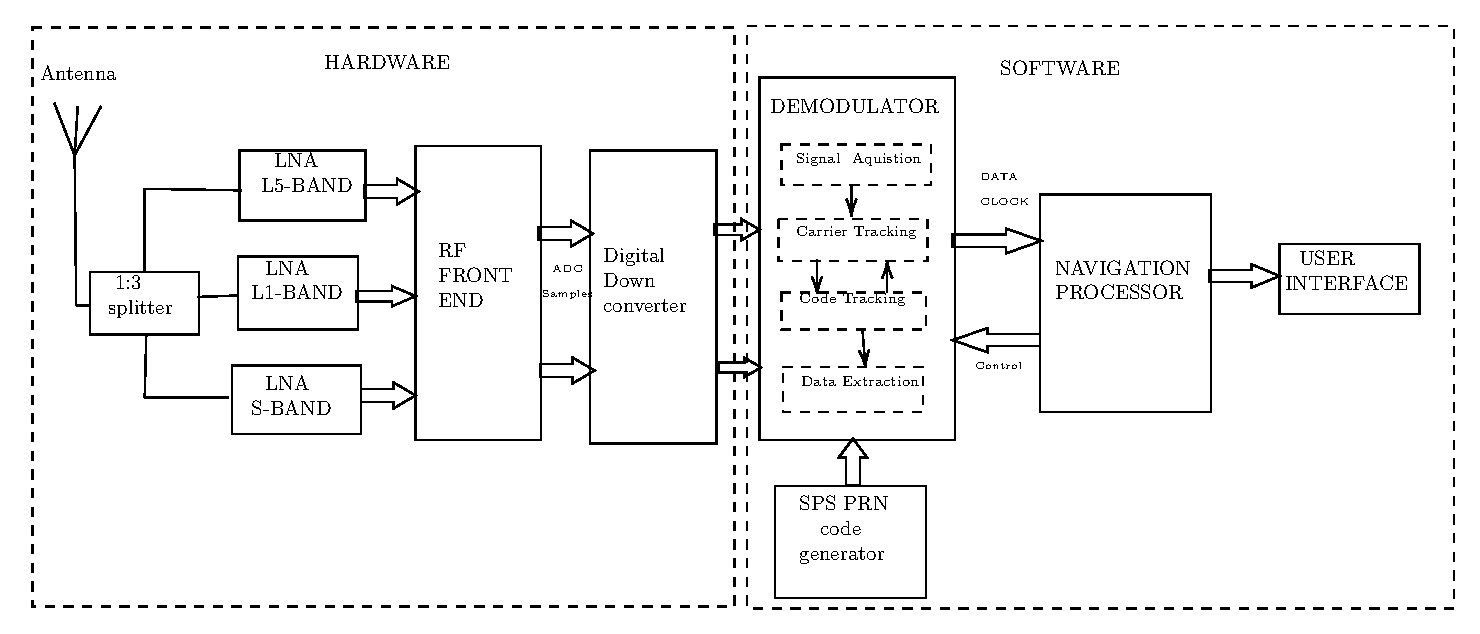
\includegraphics[scale=0.5]{figs/block1}
\caption{The Block Level Architecture}
\label{fig:Block-diagram}
\end{figure}
\section{Hardware Implementation}
\begin{figure}
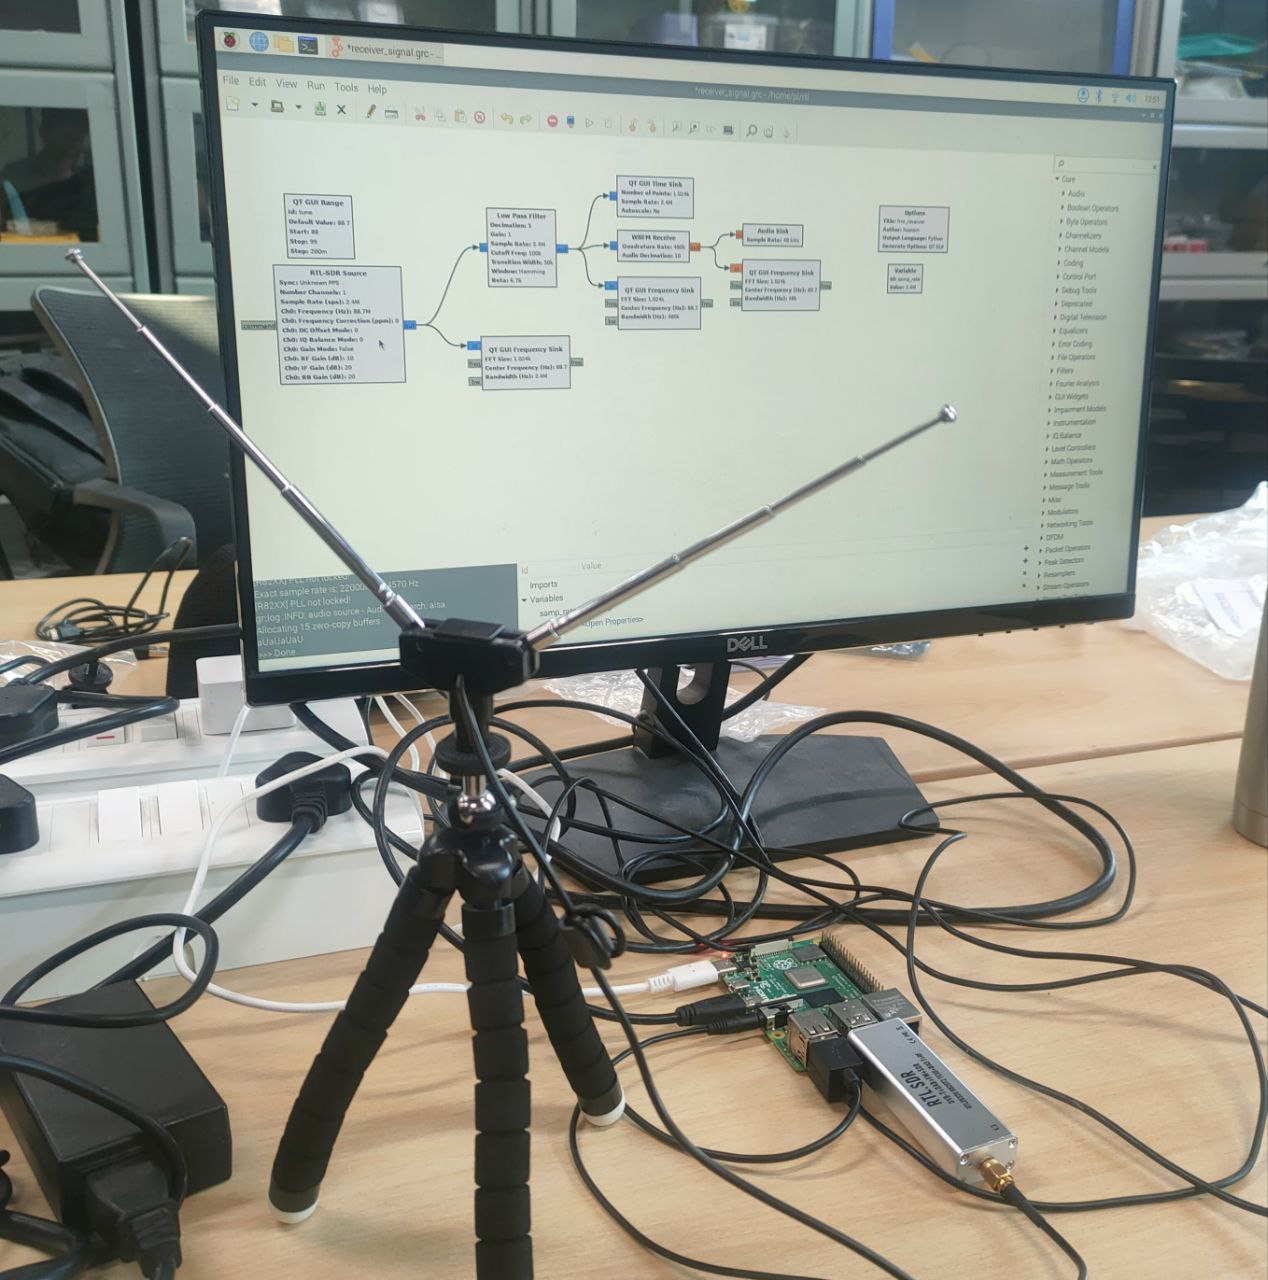
\includegraphics[scale=0.2]{figs/hardwareimplement.jpg} 
\caption{Reciever Hardware implementation}
\label{fig:hardware}
\end{figure}
List the various components used to implement receiver.
\\
\solution
\\
\begin{table}[!ht]
  \centering
 %%%%%%%%%%%%%%%%%%%%%%%%%%%%%%%%%%%%%%%%%%%%%%%%%%%%%%%%%%%%%%%%%%%%%%
%%                                                                  %%
%%  This is the header of a LaTeX2e file exported from Gnumeric.    %%
%%                                                                  %%
%%  This file can be compiled as it stands or included in another   %%
%%  LaTeX document. The table is based on the longtable package so  %%
%%  the longtable options (headers, footers...) can be set in the   %%
%%  preamble section below (see PRAMBLE).                           %%
%%                                                                  %%
%%  To include the file in another, the following two lines must be %%
%%  in the including file:                                          %%
%%        \def\inputGnumericTable{}                                 %%
%%  at the beginning of the file and:                               %%
%%        \input{name-of-this-file.tex}                             %%
%%  where the table is to be placed. Note also that the including   %%
%%  file must use the following packages for the table to be        %%
%%  rendered correctly:                                             %%
%%    \usepackage[latin1]{inputenc}                                 %%
%%    \usepackage{color}                                            %%
%%    \usepackage{array}                                            %%
%%    \usepackage{longtable}                                        %%
%%    \usepackage{calc}                                             %%
%%    \usepackage{multirow}                                         %%
%%    \usepackage{hhline}                                           %%
%%    \usepackage{ifthen}                                           %%
%%  optionally (for landscape tables embedded in another document): %%
%%    \usepackage{lscape}                                           %%
%%                                                                  %%
%%%%%%%%%%%%%%%%%%%%%%%%%%%%%%%%%%%%%%%%%%%%%%%%%%%%%%%%%%%%%%%%%%%%%%



%%  This section checks if we are begin input into another file or  %%
%%  the file will be compiled alone. First use a macro taken from   %%
%%  the TeXbook ex 7.7 (suggestion of Han-Wen Nienhuys).            %%
\def\ifundefined#1{\expandafter\ifx\csname#1\endcsname\relax}


%%  Check for the \def token for inputed files. If it is not        %%
%%  defined, the file will be processed as a standalone and the     %%
%%  preamble will be used.                                          %%
\ifundefined{inputGnumericTable}

%%  We must be able to close or not the document at the end.        %%
	\def\gnumericTableEnd{\end{document}}


%%%%%%%%%%%%%%%%%%%%%%%%%%%%%%%%%%%%%%%%%%%%%%%%%%%%%%%%%%%%%%%%%%%%%%
%%                                                                  %%
%%  This is the PREAMBLE. Change these values to get the right      %%
%%  paper size and other niceties.                                  %%
%%                                                                  %%
%%%%%%%%%%%%%%%%%%%%%%%%%%%%%%%%%%%%%%%%%%%%%%%%%%%%%%%%%%%%%%%%%%%%%%

	\documentclass[12pt%
			  %,landscape%
                    ]{report}
       \usepackage[latin1]{inputenc}
       \usepackage{fullpage}
       \usepackage{color}
       \usepackage{array}
       \usepackage{longtable}
       \usepackage{calc}
       \usepackage{multirow}
       \usepackage{hhline}
       \usepackage{ifthen}

	\begin{document}


%%  End of the preamble for the standalone. The next section is for %%
%%  documents which are included into other LaTeX2e files.          %%
\else

%%  We are not a stand alone document. For a regular table, we will %%
%%  have no preamble and only define the closing to mean nothing.   %%
    \def\gnumericTableEnd{}

%%  If we want landscape mode in an embedded document, comment out  %%
%%  the line above and uncomment the two below. The table will      %%
%%  begin on a new page and run in landscape mode.                  %%
%       \def\gnumericTableEnd{\end{landscape}}
%       \begin{landscape}


%%  End of the else clause for this file being \input.              %%
\fi

%%%%%%%%%%%%%%%%%%%%%%%%%%%%%%%%%%%%%%%%%%%%%%%%%%%%%%%%%%%%%%%%%%%%%%
%%                                                                  %%
%%  The rest is the gnumeric table, except for the closing          %%
%%  statement. Changes below will alter the table's appearance.     %%
%%                                                                  %%
%%%%%%%%%%%%%%%%%%%%%%%%%%%%%%%%%%%%%%%%%%%%%%%%%%%%%%%%%%%%%%%%%%%%%%

\providecommand{\gnumericmathit}[1]{#1} 
%%  Uncomment the next line if you would like your numbers to be in %%
%%  italics if they are italizised in the gnumeric table.           %%
%\renewcommand{\gnumericmathit}[1]{\mathit{#1}}
\providecommand{\gnumericPB}[1]%
{\let\gnumericTemp=\\#1\let\\=\gnumericTemp\hspace{0pt}}
 \ifundefined{gnumericTableWidthDefined}
        \newlength{\gnumericTableWidth}
        \newlength{\gnumericTableWidthComplete}
        \newlength{\gnumericMultiRowLength}
        \global\def\gnumericTableWidthDefined{}
 \fi
%% The following setting protects this code from babel shorthands.  %%
 \ifthenelse{\isundefined{\languageshorthands}}{}{\languageshorthands{english}}
%%  The default table format retains the relative column widths of  %%
%%  gnumeric. They can easily be changed to c, r or l. In that case %%
%%  you may want to comment out the next line and uncomment the one %%
%%  thereafter                                                      %%
\providecommand\gnumbox{\makebox[0pt]}
%%\providecommand\gnumbox[1][]{\makebox}

%% to adjust positions in multirow situations                       %%
\setlength{\bigstrutjot}{\jot}
\setlength{\extrarowheight}{\doublerulesep}

%%  The \setlongtables command keeps column widths the same across  %%
%%  pages. Simply comment out next line for varying column widths.  %%
\setlongtables

\setlength\gnumericTableWidth{%
	98pt+%
	215pt+%
	53pt+%
	53pt+%
0pt}
\def\gumericNumCols{4}
\setlength\gnumericTableWidthComplete{\gnumericTableWidth+%
         \tabcolsep*\gumericNumCols*2+\arrayrulewidth*\gumericNumCols}
\ifthenelse{\lengthtest{\gnumericTableWidthComplete > \linewidth}}%
         {\def\gnumericScale{1*\ratio{\linewidth-%
                        \tabcolsep*\gumericNumCols*2-%
                        \arrayrulewidth*\gumericNumCols}%
{\gnumericTableWidth}}}%
{\def\gnumericScale{1}}

%%%%%%%%%%%%%%%%%%%%%%%%%%%%%%%%%%%%%%%%%%%%%%%%%%%%%%%%%%%%%%%%%%%%%%
%%                                                                  %%
%% The following are the widths of the various columns. We are      %%
%% defining them here because then they are easier to change.       %%
%% Depending on the cell formats we may use them more than once.    %%
%%                                                                  %%
%%%%%%%%%%%%%%%%%%%%%%%%%%%%%%%%%%%%%%%%%%%%%%%%%%%%%%%%%%%%%%%%%%%%%%

\ifthenelse{\isundefined{\gnumericColA}}{\newlength{\gnumericColA}}{}\settowidth{\gnumericColA}{\begin{tabular}{@{}p{98pt*\gnumericScale}@{}}x\end{tabular}}
\ifthenelse{\isundefined{\gnumericColB}}{\newlength{\gnumericColB}}{}\settowidth{\gnumericColB}{\begin{tabular}{@{}p{215pt*\gnumericScale}@{}}x\end{tabular}}
\ifthenelse{\isundefined{\gnumericColC}}{\newlength{\gnumericColC}}{}\settowidth{\gnumericColC}{\begin{tabular}{@{}p{53pt*\gnumericScale}@{}}x\end{tabular}}
\ifthenelse{\isundefined{\gnumericColD}}{\newlength{\gnumericColD}}{}\settowidth{\gnumericColD}{\begin{tabular}{@{}p{53pt*\gnumericScale}@{}}x\end{tabular}}

\begin{longtable}[c]{%
	b{\gnumericColA}%
	b{\gnumericColB}%
	b{\gnumericColC}%
	b{\gnumericColD}%
	}

%%%%%%%%%%%%%%%%%%%%%%%%%%%%%%%%%%%%%%%%%%%%%%%%%%%%%%%%%%%%%%%%%%%%%%
%%  The longtable options. (Caption, headers... see Goosens, p.124) %%
%	\caption{The Table Caption.}             \\	%
% \hline	% Across the top of the table.
%%  The rest of these options are table rows which are placed on    %%
%%  the first, last or every page. Use \multicolumn if you want.    %%

%%  Header for the first page.                                      %%
%	\multicolumn{4}{c}{The First Header} \\ \hline 
%	\multicolumn{1}{c}{colTag}	%Column 1
%	&\multicolumn{1}{c}{colTag}	%Column 2
%	&\multicolumn{1}{c}{colTag}	%Column 3
%	&\multicolumn{1}{c}{colTag}	\\ \hline %Last column
%	\endfirsthead

%%  The running header definition.                                  %%
%	\hline
%	\multicolumn{4}{l}{\ldots\small\slshape continued} \\ \hline
%	\multicolumn{1}{c}{colTag}	%Column 1
%	&\multicolumn{1}{c}{colTag}	%Column 2
%	&\multicolumn{1}{c}{colTag}	%Column 3
%	&\multicolumn{1}{c}{colTag}	\\ \hline %Last column
%	\endhead

%%  The running footer definition.                                  %%
%	\hline
%	\multicolumn{4}{r}{\small\slshape continued\ldots} \\
%	\endfoot

%%  The ending footer definition.                                   %%
%	\multicolumn{4}{c}{That's all folks} \\ \hline 
%	\endlastfoot
%%%%%%%%%%%%%%%%%%%%%%%%%%%%%%%%%%%%%%%%%%%%%%%%%%%%%%%%%%%%%%%%%%%%%%

\hhline{|-|-|--}
	 \multicolumn{1}{|p{\gnumericColA}|}%
	{\gnumericPB{\centering}\gnumbox{\textbf{Component}}}
	&\multicolumn{1}{p{\gnumericColB}|}%
	{\gnumericPB{\centering}\gnumbox{\textbf{Type}}}
	
\\
\hhline{|----|}
	 \multicolumn{1}{|p{\gnumericColA}|}%
	{\gnumericPB{\centering}\gnumbox{RTL-SDR chip}}
	&\multicolumn{1}{p{\gnumericColB}|}%
	{\gnumericPB{\raggedright}\gnumbox[l]{Hardware}}
	
\\
\hhline{|----|}
	 \multicolumn{1}{|p{\gnumericColA}|}%
	{\gnumericPB{\centering}\gnumbox{GNU radio}}
	&\multicolumn{1}{p{\gnumericColB}|}%
	{\gnumericPB{\raggedright}\gnumbox[l]{Software}}
	
\\
\hhline{|----|}
	 \multicolumn{1}{|p{\gnumericColA}|}%
	{\gnumericPB{\centering}\gnumbox{Antenna}}
	&\multicolumn{1}{p{\gnumericColB}|}%
	{\gnumericPB{\raggedright}\gnumbox[l]{Hardware}}
	

\\
\hhline{|-|-|--|}
\end{longtable}

\ifthenelse{\isundefined{\languageshorthands}}{}{\languageshorthands{\languagename}}
\gnumericTableEnd

  \caption{Components Required}
  \label{tab:rxcomponents}
\end{table}
Components are listed in the table \tabref{tab:rxcomponents}\\
The picture of RTL-SDR and Antenna is given in \figref{fig:hardware}.This set is used to receive the L5,L1,S Band  signals.
\begin{figure}[ht]
\centering
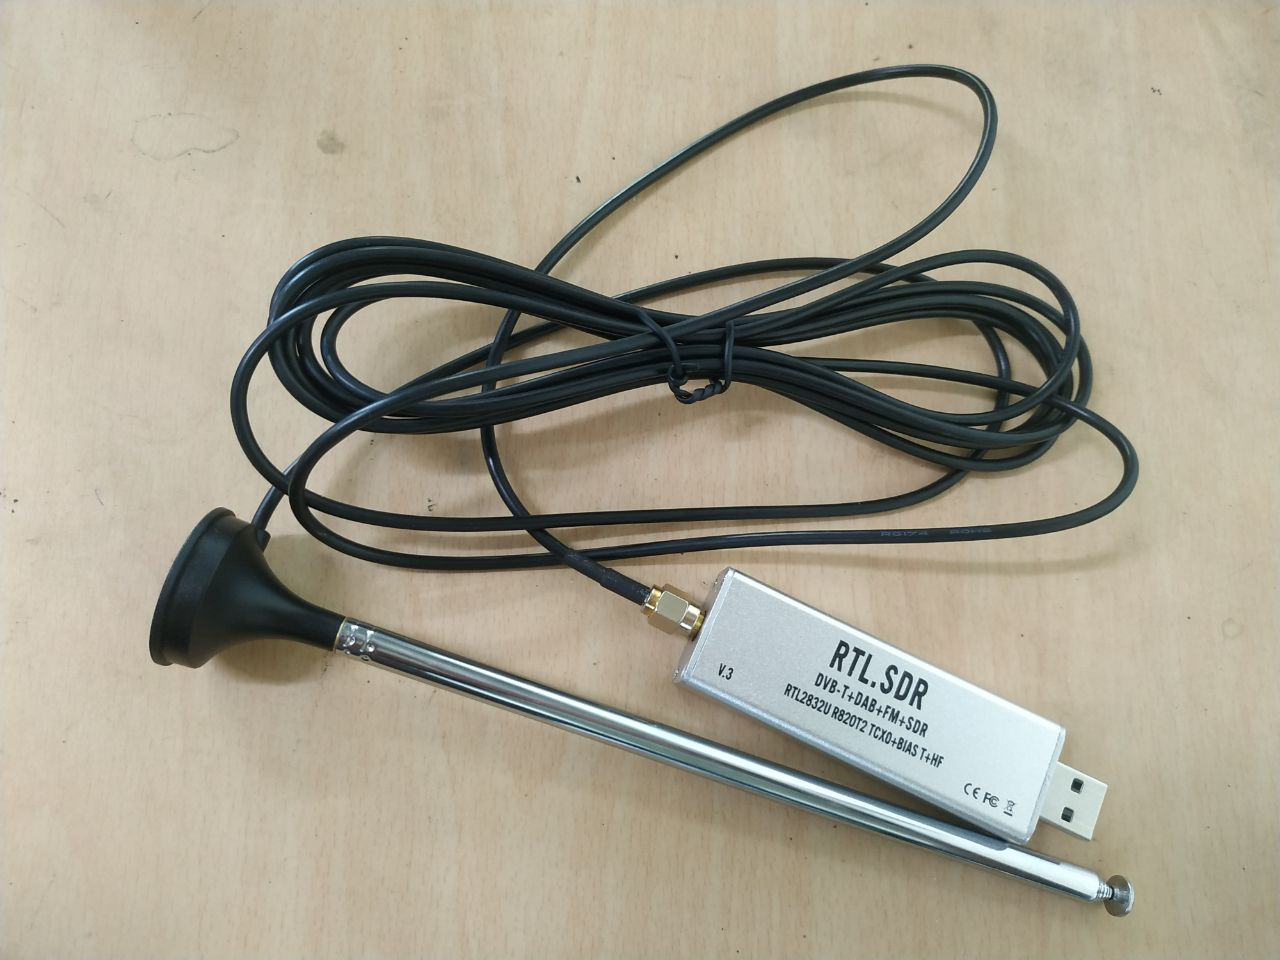
\includegraphics[width=0.5\columnwidth]{figs/rtl-sdr.png}
\caption{RTL-SDR}
\label{fig:rtl-sdr}
\end{figure}
\section{RTL SDR Specifications}
RTL-SDR is a popular, low cost hardware that can receive wireless signals. The RTL-SDR dongle features the Realtek RTL2838U chip, which provides I-Q samples through the USB interface. 
\begin{table}[!ht]
  \centering
 %%%%%%%%%%%%%%%%%%%%%%%%%%%%%%%%%%%%%%%%%%%%%%%%%%%%%%%%%%%%%%%%%%%%%%
%%                                                                  %%
%%  This is the header of a LaTeX2e file exported from Gnumeric.    %%
%%                                                                  %%
%%  This file can be compiled as it stands or included in another   %%
%%  LaTeX document. The table is based on the longtable package so  %%
%%  the longtable options (headers, footers...) can be set in the   %%
%%  preamble section below (see PRAMBLE).                           %%
%%                                                                  %%
%%  To include the file in another, the following two lines must be %%
%%  in the including file:                                          %%
%%        \def\inputGnumericTable{}                                 %%
%%  at the beginning of the file and:                               %%
%%        \input{name-of-this-file.tex}                             %%
%%  where the table is to be placed. Note also that the including   %%
%%  file must use the following packages for the table to be        %%
%%  rendered correctly:                                             %%
%%    \usepackage[latin1]{inputenc}                                 %%
%%    \usepackage{color}                                            %%
%%    \usepackage{array}                                            %%
%%    \usepackage{longtable}                                        %%
%%    \usepackage{calc}                                             %%
%%    \usepackage{multirow}                                         %%
%%    \usepackage{hhline}                                           %%
%%    \usepackage{ifthen}                                           %%
%%  optionally (for landscape tables embedded in another document): %%
%%    \usepackage{lscape}                                           %%
%%                                                                  %%
%%%%%%%%%%%%%%%%%%%%%%%%%%%%%%%%%%%%%%%%%%%%%%%%%%%%%%%%%%%%%%%%%%%%%%



%%  This section checks if we are begin input into another file or  %%
%%  the file will be compiled alone. First use a macro taken from   %%
%%  the TeXbook ex 7.7 (suggestion of Han-Wen Nienhuys).            %%
\def\ifundefined#1{\expandafter\ifx\csname#1\endcsname\relax}


%%  Check for the \def token for inputed files. If it is not        %%
%%  defined, the file will be processed as a standalone and the     %%
%%  preamble will be used.                                          %%
\ifundefined{inputGnumericTable}

%%  We must be able to close or not the document at the end.        %%
	\def\gnumericTableEnd{\end{document}}


%%%%%%%%%%%%%%%%%%%%%%%%%%%%%%%%%%%%%%%%%%%%%%%%%%%%%%%%%%%%%%%%%%%%%%
%%                                                                  %%
%%  This is the PREAMBLE. Change these values to get the right      %%
%%  paper size and other niceties.                                  %%
%%                                                                  %%
%%%%%%%%%%%%%%%%%%%%%%%%%%%%%%%%%%%%%%%%%%%%%%%%%%%%%%%%%%%%%%%%%%%%%%

	\documentclass[12pt%
			  %,landscape%
                    ]{report}
       \usepackage[latin1]{inputenc}
       \usepackage{fullpage}
       \usepackage{color}
       \usepackage{array}
       \usepackage{longtable}
       \usepackage{calc}
       \usepackage{multirow}
       \usepackage{hhline}
       \usepackage{ifthen}

	\begin{document}


%%  End of the preamble for the standalone. The next section is for %%
%%  documents which are included into other LaTeX2e files.          %%
\else

%%  We are not a stand alone document. For a regular table, we will %%
%%  have no preamble and only define the closing to mean nothing.   %%
    \def\gnumericTableEnd{}

%%  If we want landscape mode in an embedded document, comment out  %%
%%  the line above and uncomment the two below. The table will      %%
%%  begin on a new page and run in landscape mode.                  %%
%       \def\gnumericTableEnd{\end{landscape}}
%       \begin{landscape}


%%  End of the else clause for this file being \input.              %%
\fi

%%%%%%%%%%%%%%%%%%%%%%%%%%%%%%%%%%%%%%%%%%%%%%%%%%%%%%%%%%%%%%%%%%%%%%
%%                                                                  %%
%%  The rest is the gnumeric table, except for the closing          %%
%%  statement. Changes below will alter the table's appearance.     %%
%%                                                                  %%
%%%%%%%%%%%%%%%%%%%%%%%%%%%%%%%%%%%%%%%%%%%%%%%%%%%%%%%%%%%%%%%%%%%%%%

\providecommand{\gnumericmathit}[1]{#1} 
%%  Uncomment the next line if you would like your numbers to be in %%
%%  italics if they are italizised in the gnumeric table.           %%
%\renewcommand{\gnumericmathit}[1]{\mathit{#1}}
\providecommand{\gnumericPB}[1]%
{\let\gnumericTemp=\\#1\let\\=\gnumericTemp\hspace{0pt}}
 \ifundefined{gnumericTableWidthDefined}
        \newlength{\gnumericTableWidth}
        \newlength{\gnumericTableWidthComplete}
        \newlength{\gnumericMultiRowLength}
        \global\def\gnumericTableWidthDefined{}
 \fi
%% The following setting protects this code from babel shorthands.  %%
 \ifthenelse{\isundefined{\languageshorthands}}{}{\languageshorthands{english}}
%%  The default table format retains the relative column widths of  %%
%%  gnumeric. They can easily be changed to c, r or l. In that case %%
%%  you may want to comment out the next line and uncomment the one %%
%%  thereafter                                                      %%
\providecommand\gnumbox{\makebox[0pt]}
%%\providecommand\gnumbox[1][]{\makebox}

%% to adjust positions in multirow situations                       %%
\setlength{\bigstrutjot}{\jot}
\setlength{\extrarowheight}{\doublerulesep}

%%  The \setlongtables command keeps column widths the same across  %%
%%  pages. Simply comment out next line for varying column widths.  %%
\setlongtables

\setlength\gnumericTableWidth{%
	95pt+%
	235pt+%
0pt}
\def\gumericNumCols{2}
\setlength\gnumericTableWidthComplete{\gnumericTableWidth+%
         \tabcolsep*\gumericNumCols*2+\arrayrulewidth*\gumericNumCols}
\ifthenelse{\lengthtest{\gnumericTableWidthComplete > \linewidth}}%
         {\def\gnumericScale{\ratio{\linewidth-%
                        \tabcolsep*\gumericNumCols*2-%
                        \arrayrulewidth*\gumericNumCols}%
{\gnumericTableWidth}}}%
{\def\gnumericScale{1}}

%%%%%%%%%%%%%%%%%%%%%%%%%%%%%%%%%%%%%%%%%%%%%%%%%%%%%%%%%%%%%%%%%%%%%%
%%                                                                  %%
%% The following are the widths of the various columns. We are      %%
%% defining them here because then they are easier to change.       %%
%% Depending on the cell formats we may use them more than once.    %%
%%                                                                  %%
%%%%%%%%%%%%%%%%%%%%%%%%%%%%%%%%%%%%%%%%%%%%%%%%%%%%%%%%%%%%%%%%%%%%%%

\ifthenelse{\isundefined{\gnumericColA}}{\newlength{\gnumericColA}}{}\settowidth{\gnumericColA}{\begin{tabular}{@{}p{95pt*\gnumericScale}@{}}x\end{tabular}}
\ifthenelse{\isundefined{\gnumericColB}}{\newlength{\gnumericColB}}{}\settowidth{\gnumericColB}{\begin{tabular}{@{}p{235pt*\gnumericScale}@{}}x\end{tabular}}

\begin{longtable}[c]{%
	b{\gnumericColA}%
	b{\gnumericColB}%
	}

%%%%%%%%%%%%%%%%%%%%%%%%%%%%%%%%%%%%%%%%%%%%%%%%%%%%%%%%%%%%%%%%%%%%%%
%%  The longtable options. (Caption, headers... see Goosens, p.124) %%
%	\caption{The Table Caption.}             \\	%
% \hline	% Across the top of the table.
%%  The rest of these options are table rows which are placed on    %%
%%  the first, last or every page. Use \multicolumn if you want.    %%

%%  Header for the first page.                                      %%
%	\multicolumn{2}{c}{The First Header} \\ \hline 
%	\multicolumn{1}{c}{colTag}	%Column 1
%	&\multicolumn{1}{c}{colTag}	\\ \hline %Last column
%	\endfirsthead

%%  The running header definition.                                  %%
%	\hline
%	\multicolumn{2}{l}{\ldots\small\slshape continued} \\ \hline
%	\multicolumn{1}{c}{colTag}	%Column 1
%	&\multicolumn{1}{c}{colTag}	\\ \hline %Last column
%	\endhead

%%  The running footer definition.                                  %%
%	\hline
%	\multicolumn{2}{r}{\small\slshape continued\ldots} \\
%	\endfoot

%%  The ending footer definition.                                   %%
%	\multicolumn{2}{c}{That's all folks} \\ \hline 
%	\endlastfoot
%%%%%%%%%%%%%%%%%%%%%%%%%%%%%%%%%%%%%%%%%%%%%%%%%%%%%%%%%%%%%%%%%%%%%%

\hhline{|-|-}
	 \multicolumn{1}{|p{\gnumericColA}|}%
	{\gnumericPB{\raggedright}\gnumbox[l]{\hspace{0.75cm}\textbf{Name}}}
	&\multicolumn{1}{p{\gnumericColB}|}%
	{\gnumericPB{\raggedright}\gnumbox[l]{ \textbf{RTL-SDR(R820T2/RTL2838U DVB-T)}}}
\\
\hhline{|--|}
	 \multicolumn{1}{|p{\gnumericColA}|}%
	{\gnumericPB{\raggedright}\gnumbox[l]{Type}}
	&\multicolumn{1}{p{\gnumericColB}|}%
	{\gnumericPB{\raggedright}\gnumbox[l]{Pre-built and premodded with custom driver}}
\\
\hhline{|--|}
	 \multicolumn{1}{|p{\gnumericColA}|}%
	{\gnumericPB{\raggedright}\gnumbox[l]{Frequency range}}
	&\multicolumn{1}{p{\gnumericColB}|}%
	{\gnumericPB{\raggedright}\gnumbox[l]{0.5-1766MHz}}
\\
\hhline{|--|}
	 \multicolumn{1}{|p{\gnumericColA}|}%
	{\gnumericPB{\raggedright}\gnumbox[l]{Max Bandwidth}}
	&\multicolumn{1}{p{\gnumericColB}|}%
	{\gnumericPB{\raggedright}\gnumbox[l]{Matches sampling rate but with filter roll-off}}
\\
\hhline{|--|}
	 \multicolumn{1}{|p{\gnumericColA}|}%
	{\gnumericPB{\raggedright}\gnumbox[l]{Receiver ADC bits }}
	&\multicolumn{1}{p{\gnumericColB}|}%
	{\gnumericPB{\raggedright}\gnumbox[l]{8}}
\\
\hhline{|--|}
	 \multicolumn{1}{|p{\gnumericColA}|}%
	{\gnumericPB{\raggedright}\gnumbox[l]{Tx.DAC bits}}
	&\multicolumn{1}{p{\gnumericColB}|}%
	{\gnumericPB{\raggedright}\gnumbox[l]{-}}
\\
\hhline{|--|}
	 \multicolumn{1}{|p{\gnumericColA}|}%
	{\gnumericPB{\raggedright}\gnumbox[l]{Tx. Cable }}
	&\multicolumn{1}{p{\gnumericColB}|}%
	{\gnumericPB{\raggedright}\gnumbox[l]{No}}
\\
\hhline{|--|}
	 \multicolumn{1}{|p{\gnumericColA}|}%
	{\gnumericPB{\raggedright}\gnumbox[l]{Sampling Rate }}
	&\multicolumn{1}{p{\gnumericColB}|}%
	{\gnumericPB{\raggedright}\gnumbox[l]{2.4 MHz }}
\\
\hhline{|-|-|}
\multicolumn{1}{|p{\gnumericColA}|}%
	{\gnumericPB{\raggedright}\gnumbox[l]{Frequency accuracy }}
	&\multicolumn{1}{p{\gnumericColB}|}%
	{\gnumericPB{\raggedright}\gnumbox[l]{1 ppm}}
\\
\hhline{|--|}
	 \multicolumn{1}{|p{\gnumericColA}|}%
	{\gnumericPB{\raggedright}\gnumbox[l]{Host inerface }}
	&\multicolumn{1}{p{\gnumericColB}|}%
	{\gnumericPB{\raggedright}\gnumbox[l]{USB }}
\\
\hhline{|--|}
	 \multicolumn{1}{|p{\gnumericColA}|}%
	{\gnumericPB{\raggedright}\gnumbox[l]{FPGA}}
	&\multicolumn{1}{p{\gnumericColB}|}%
	{\gnumericPB{\raggedright}\gnumbox[l]{-}}
\\

\hhline{|--|}
\end{longtable}

\ifthenelse{\isundefined{\languageshorthands}}{}{\languageshorthands{\languagename}}
\gnumericTableEnd

  \caption{RTL-SDR Specification table }
  \label{tab:rxspecification}
\end{table}

 Install and open GNU Radio using the following commands
\\
\begin{lstlisting}
sudo apt update
sudo apt install gnuradio
gnuradio-companion
\end{lstlisting}
 How to construct the block diagram in GNU radio? \\
	\solution  \\
\textbf{Step-1}:\\
Search for QTGUI Time sink  block and add it to the work space.
\begin{figure}[ht]
\centering
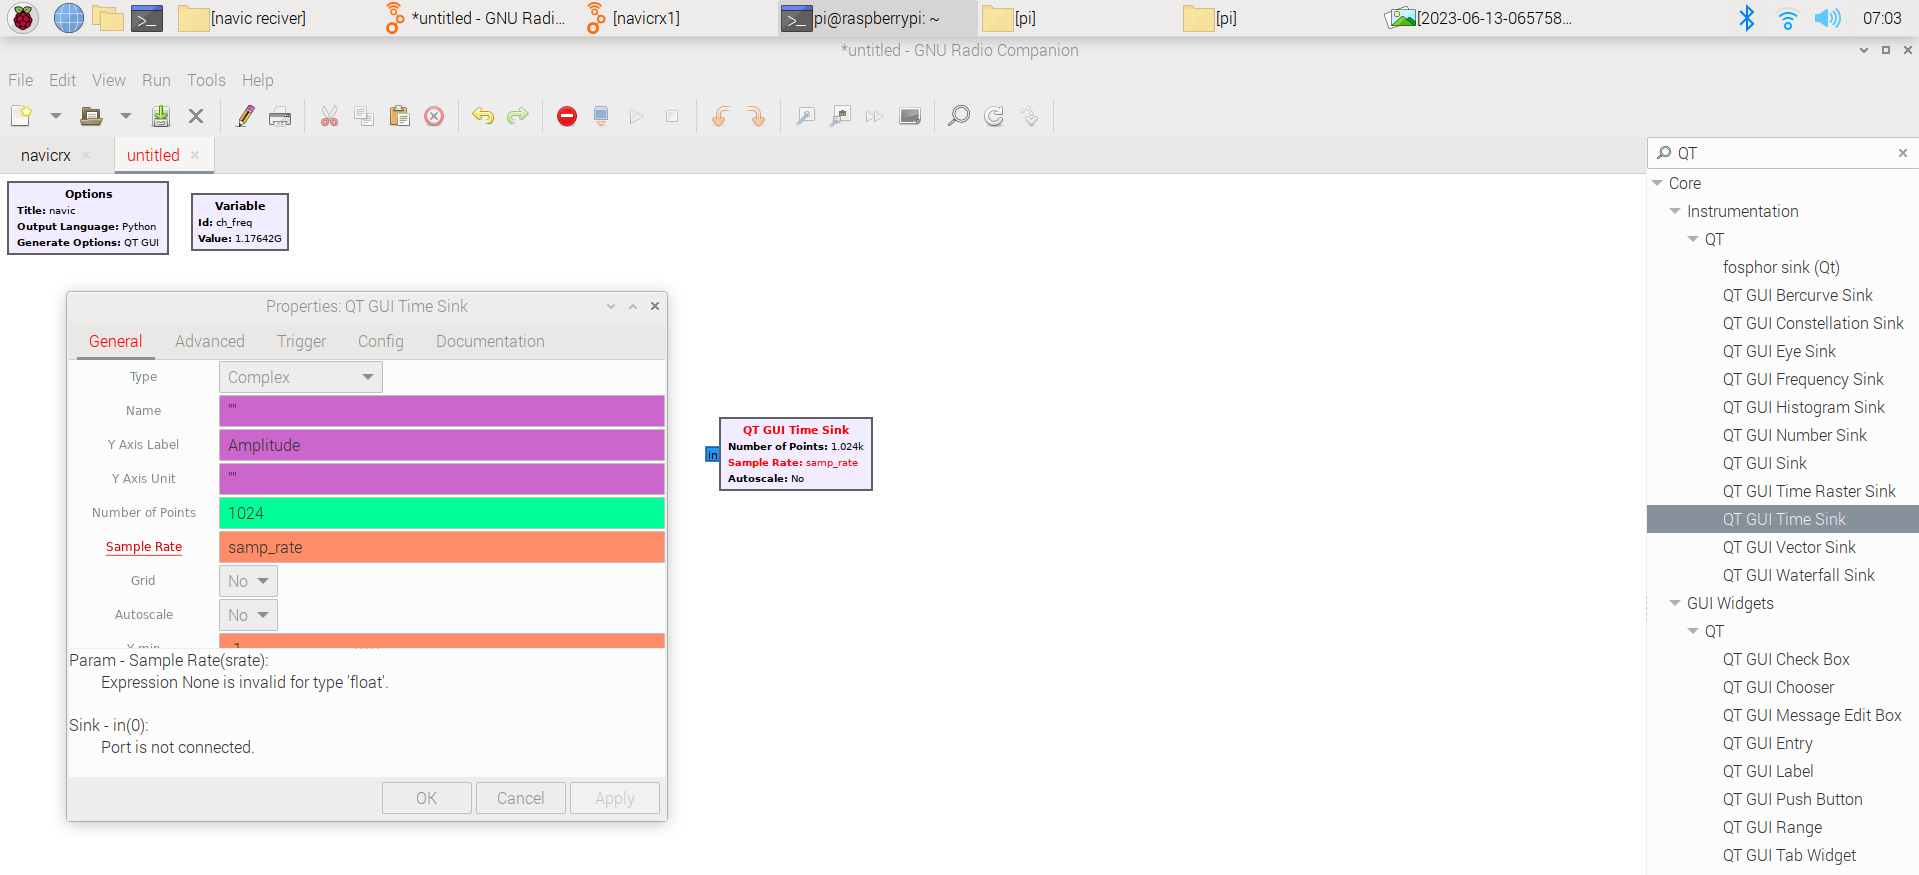
\includegraphics[width=\columnwidth]{figs/add.png}
\caption{Adding blocks}
\label{fig:add blocks}
\end{figure}
\textbf{Step-2}:
Similarly do for RTL-Source block,complex to real ,complex to imaginary and QTGUI Time sink block.
\\
\textbf{Step-3}:
Change the parameters in each block according your values by double clicking on it.
\\
\textbf{Step-4}:
Connect them according to the flowgraph shown in \figref{fig:Rx_Block_diagram}.
\begin{figure}[ht]
\centering
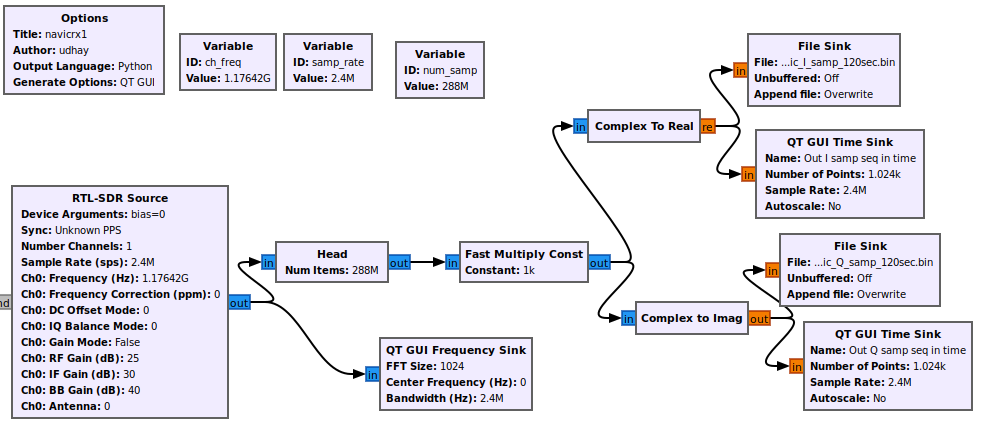
\includegraphics[width=\columnwidth]{figs/RTL_SDR_test.png}
\caption{Block diagram of Receiver in GNU Radio}
\label{fig:Rx_Block_diagram}
\end{figure}
\textbf{Note}:
Refer the following website for any queries.
\begin{lstlisting}
https://wiki.gnuradio.org/index.php?title=Creating_Your_First_Block
\end{lstlisting}
 Explain each block in block diagram of Receiver.\\
	\solution \\
\textbf{1. RTL-SDR Source}:\\
The RTL-SDR Source block is used to stream samples from RTL-SDR device.
\begin{figure}[ht]
\centering
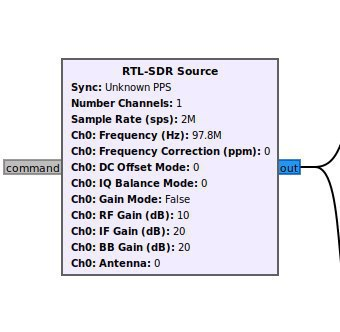
\includegraphics[width=0.4\columnwidth]{figs/source_block.png}
\caption{RTL-SDR Source Block}
\label{fig:source block_RTL}
\end{figure}
Connect the RTL-SDR to the system and execute the flowgraph in \figref{fig:Rx_Block_diagram}.\\



\subsection{Results} 
\begin{figure}
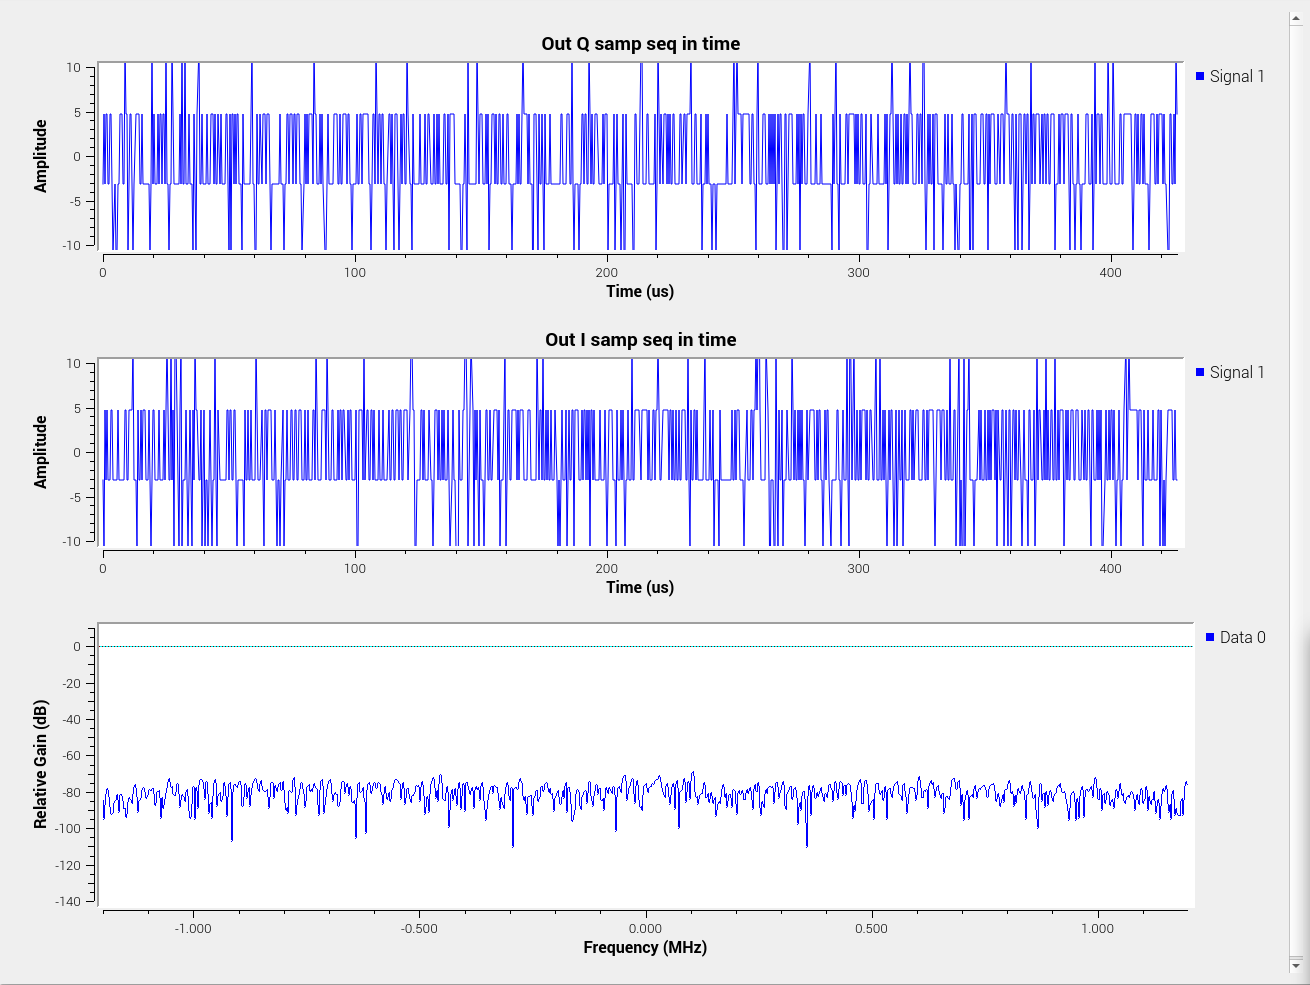
\includegraphics[width=0.8\columnwidth]{figs/RTL_sdr_res.png}
\caption{RTL-SDR receiver plots}
\end{figure}
I,Q samples will be stored in a file with .bin extension

 Read the data from RTL SDR stored in .bin file using python code and without using GNU radio.
\\
\solution \\
The following code reads the data from RTL-SDR without GNU radio.
\begin{lstlisting}
codes/receiver/rtsdr_rx.py
\end{lstlisting}














\section{USRP SDR}
The picture of Universal software Radio Peripheral-software defiend radios (USRP-SDR)  is given in \figref{fig:USRP-SDR}.This set is used to receive the L5,L1,S Band  signals.
\begin{figure}[ht]
\centering
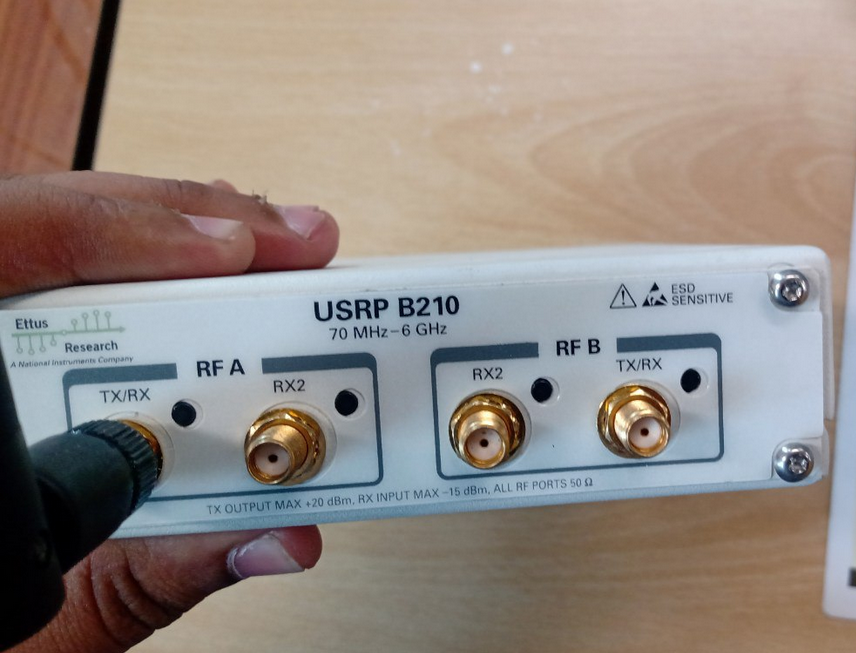
\includegraphics[width=0.5\columnwidth]{figs/USRP.png}
\caption{USRP-SDR}
\label{fig:USRP-SDR}
\end{figure}

\subsection{ USRP SDR specification}
 \begin{table}[!ht]
  \centering
 %%%%%%%%%%%%%%%%%%%%%%%%%%%%%%%%%%%%%%%%%%%%%%%%%%%%%%%%%%%%%%%%%%%%%%
%%                                                                  %%
%%  This is the header of a LaTeX2e file exported from Gnumeric.    %%
%%                                                                  %%
%%  This file can be compiled as it stands or included in another   %%
%%  LaTeX document. The table is based on the longtable package so  %%
%%  the longtable options (headers, footers...) can be set in the   %%
%%  preamble section below (see PRAMBLE).                           %%
%%                                                                  %%
%%  To include the file in another, the following two lines must be %%
%%  in the including file:                                          %%
%%        \def\inputGnumericTable{}                                 %%
%%  at the beginning of the file and:                               %%
%%        \input{name-of-this-file.tex}                             %%
%%  where the table is to be placed. Note also that the including   %%
%%  file must use the following packages for the table to be        %%
%%  rendered correctly:                                             %%
%%    \usepackage[latin1]{inputenc}                                 %%
%%    \usepackage{color}                                            %%
%%    \usepackage{array}                                            %%
%%    \usepackage{longtable}                                        %%
%%    \usepackage{calc}                                             %%
%%    \usepackage{multirow}                                         %%
%%    \usepackage{hhline}                                           %%
%%    \usepackage{ifthen}                                           %%
%%  optionally (for landscape tables embedded in another document): %%
%%    \usepackage{lscape}                                           %%
%%                                                                  %%
%%%%%%%%%%%%%%%%%%%%%%%%%%%%%%%%%%%%%%%%%%%%%%%%%%%%%%%%%%%%%%%%%%%%%%



%%  This section checks if we are begin input into another file or  %%
%%  the file will be compiled alone. First use a macro taken from   %%
%%  the TeXbook ex 7.7 (suggestion of Han-Wen Nienhuys).            %%
\def\ifundefined#1{\expandafter\ifx\csname#1\endcsname\relax}


%%  Check for the \def token for inputed files. If it is not        %%
%%  defined, the file will be processed as a standalone and the     %%
%%  preamble will be used.                                          %%
\ifundefined{inputGnumericTable}

%%  We must be able to close or not the document at the end.        %%
	\def\gnumericTableEnd{\end{document}}


%%%%%%%%%%%%%%%%%%%%%%%%%%%%%%%%%%%%%%%%%%%%%%%%%%%%%%%%%%%%%%%%%%%%%%
%%                                                                  %%
%%  This is the PREAMBLE. Change these values to get the right      %%
%%  paper size and other niceties.                                  %%
%%                                                                  %%
%%%%%%%%%%%%%%%%%%%%%%%%%%%%%%%%%%%%%%%%%%%%%%%%%%%%%%%%%%%%%%%%%%%%%%

	\documentclass[12pt%
			  %,landscape%
                    ]{report}
       \usepackage[latin1]{inputenc}
       \usepackage{fullpage}
       \usepackage{color}
       \usepackage{array}
       \usepackage{longtable}
       \usepackage{calc}
       \usepackage{multirow}
       \usepackage{hhline}
       \usepackage{ifthen}

	\begin{document}


%%  End of the preamble for the standalone. The next section is for %%
%%  documents which are included into other LaTeX2e files.          %%
\else

%%  We are not a stand alone document. For a regular table, we will %%
%%  have no preamble and only define the closing to mean nothing.   %%
    \def\gnumericTableEnd{}

%%  If we want landscape mode in an embedded document, comment out  %%
%%  the line above and uncomment the two below. The table will      %%
%%  begin on a new page and run in landscape mode.                  %%
%       \def\gnumericTableEnd{\end{landscape}}
%       \begin{landscape}


%%  End of the else clause for this file being \input.              %%
\fi

%%%%%%%%%%%%%%%%%%%%%%%%%%%%%%%%%%%%%%%%%%%%%%%%%%%%%%%%%%%%%%%%%%%%%%
%%                                                                  %%
%%  The rest is the gnumeric table, except for the closing          %%
%%  statement. Changes below will alter the table's appearance.     %%
%%                                                                  %%
%%%%%%%%%%%%%%%%%%%%%%%%%%%%%%%%%%%%%%%%%%%%%%%%%%%%%%%%%%%%%%%%%%%%%%

\providecommand{\gnumericmathit}[1]{#1} 
%%  Uncomment the next line if you would like your numbers to be in %%
%%  italics if they are italizised in the gnumeric table.           %%
%\renewcommand{\gnumericmathit}[1]{\mathit{#1}}
\providecommand{\gnumericPB}[1]%
{\let\gnumericTemp=\\#1\let\\=\gnumericTemp\hspace{0pt}}
 \ifundefined{gnumericTableWidthDefined}
        \newlength{\gnumericTableWidth}
        \newlength{\gnumericTableWidthComplete}
        \newlength{\gnumericMultiRowLength}
        \global\def\gnumericTableWidthDefined{}
 \fi
%% The following setting protects this code from babel shorthands.  %%
 \ifthenelse{\isundefined{\languageshorthands}}{}{\languageshorthands{english}}
%%  The default table format retains the relative column widths of  %%
%%  gnumeric. They can easily be changed to c, r or l. In that case %%
%%  you may want to comment out the next line and uncomment the one %%
%%  thereafter                                                      %%
\providecommand\gnumbox{\makebox[0pt]}
%%\providecommand\gnumbox[1][]{\makebox}

%% to adjust positions in multirow situations                       %%
\setlength{\bigstrutjot}{\jot}
\setlength{\extrarowheight}{\doublerulesep}

%%  The \setlongtables command keeps column widths the same across  %%
%%  pages. Simply comment out next line for varying column widths.  %%
\setlongtables

\setlength\gnumericTableWidth{%
	95pt+%
	180pt+%
0pt}
\def\gumericNumCols{2}
\setlength\gnumericTableWidthComplete{\gnumericTableWidth+%
         \tabcolsep*\gumericNumCols*2+\arrayrulewidth*\gumericNumCols}
\ifthenelse{\lengthtest{\gnumericTableWidthComplete > \linewidth}}%
         {\def\gnumericScale{\ratio{\linewidth-%
                        \tabcolsep*\gumericNumCols*2-%
                        \arrayrulewidth*\gumericNumCols}%
{\gnumericTableWidth}}}%
{\def\gnumericScale{1}}

%%%%%%%%%%%%%%%%%%%%%%%%%%%%%%%%%%%%%%%%%%%%%%%%%%%%%%%%%%%%%%%%%%%%%%
%%                                                                  %%
%% The following are the widths of the various columns. We are      %%
%% defining them here because then they are easier to change.       %%
%% Depending on the cell formats we may use them more than once.    %%
%%                                                                  %%
%%%%%%%%%%%%%%%%%%%%%%%%%%%%%%%%%%%%%%%%%%%%%%%%%%%%%%%%%%%%%%%%%%%%%%

\ifthenelse{\isundefined{\gnumericColA}}{\newlength{\gnumericColA}}{}\settowidth{\gnumericColA}{\begin{tabular}{@{}p{95pt*\gnumericScale}@{}}x\end{tabular}}
\ifthenelse{\isundefined{\gnumericColB}}{\newlength{\gnumericColB}}{}\settowidth{\gnumericColB}{\begin{tabular}{@{}p{180pt*\gnumericScale}@{}}x\end{tabular}}

\begin{longtable}[c]{%
	b{\gnumericColA}%
	b{\gnumericColB}%
	}

%%%%%%%%%%%%%%%%%%%%%%%%%%%%%%%%%%%%%%%%%%%%%%%%%%%%%%%%%%%%%%%%%%%%%%
%%  The longtable options. (Caption, headers... see Goosens, p.124) %%
%	\caption{The Table Caption.}             \\	%
% \hline	% Across the top of the table.
%%  The rest of these options are table rows which are placed on    %%
%%  the first, last or every page. Use \multicolumn if you want.    %%

%%  Header for the first page.                                      %%
%	\multicolumn{2}{c}{The First Header} \\ \hline 
%	\multicolumn{1}{c}{colTag}	%Column 1
%	&\multicolumn{1}{c}{colTag}	\\ \hline %Last column
%	\endfirsthead

%%  The running header definition.                                  %%
%	\hline
%	\multicolumn{2}{l}{\ldots\small\slshape continued} \\ \hline
%	\multicolumn{1}{c}{colTag}	%Column 1
%	&\multicolumn{1}{c}{colTag}	\\ \hline %Last column
%	\endhead

%%  The running footer definition.                                  %%
%	\hline
%	\multicolumn{2}{r}{\small\slshape continued\ldots} \\
%	\endfoot

%%  The ending footer definition.                                   %%
%	\multicolumn{2}{c}{That's all folks} \\ \hline 
%	\endlastfoot
%%%%%%%%%%%%%%%%%%%%%%%%%%%%%%%%%%%%%%%%%%%%%%%%%%%%%%%%%%%%%%%%%%%%%%

\hhline{|-|-}
	 \multicolumn{1}{|p{\gnumericColA}|}%
	{\gnumericPB{\raggedright}\gnumbox[l]{\hspace{0.75cm}\textbf{Name}}}
	&\multicolumn{1}{p{\gnumericColB}|}%
	{\gnumericPB{\raggedright}\gnumbox[l]{ \textbf{USRP B210}}}
\\
\hhline{|--|}
	 \multicolumn{1}{|p{\gnumericColA}|}%
	{\gnumericPB{\raggedright}\gnumbox[l]{Type}}
	&\multicolumn{1}{p{\gnumericColB}|}%
	{\gnumericPB{\raggedright}\gnumbox[l]{Pre-built}}
\\
\hhline{|--|}
	 \multicolumn{1}{|p{\gnumericColA}|}%
	{\gnumericPB{\raggedright}\gnumbox[l]{Frequency range}}
	&\multicolumn{1}{p{\gnumericColB}|}%
	{\gnumericPB{\raggedright}\gnumbox[l]{70MHz-6GHz}}
\\
\hhline{|--|}
	 \multicolumn{1}{|p{\gnumericColA}|}%
	{\gnumericPB{\raggedright}\gnumbox[l]{Max Bandwidth}}
	&\multicolumn{1}{p{\gnumericColB}|}%
	{\gnumericPB{\raggedright}\gnumbox[l]{56MHz}}
\\
\hhline{|--|}
	 \multicolumn{1}{|p{\gnumericColA}|}%
	{\gnumericPB{\raggedright}\gnumbox[l]{Receiver ADC bits }}
	&\multicolumn{1}{p{\gnumericColB}|}%
	{\gnumericPB{\raggedright}\gnumbox[l]{12}}
\\
\hhline{|--|}
	 \multicolumn{1}{|p{\gnumericColA}|}%
	{\gnumericPB{\raggedright}\gnumbox[l]{Tx.DAC bits}}
	&\multicolumn{1}{p{\gnumericColB}|}%
	{\gnumericPB{\raggedright}\gnumbox[l]{12}}
\\
\hhline{|--|}
	 \multicolumn{1}{|p{\gnumericColA}|}%
	{\gnumericPB{\raggedright}\gnumbox[l]{Tx. Cable }}
	&\multicolumn{1}{p{\gnumericColB}|}%
	{\gnumericPB{\raggedright}\gnumbox[l]{Yes}}
\\
\hhline{|--|}
	 \multicolumn{1}{|p{\gnumericColA}|}%
	{\gnumericPB{\raggedright}\gnumbox[l]{Sampling Rate }}
	&\multicolumn{1}{p{\gnumericColB}|}%
	{\gnumericPB{\raggedright}\gnumbox[l]{50 Msps }}
\\
\hhline{|-|-|}
\multicolumn{1}{|p{\gnumericColA}|}%
	{\gnumericPB{\raggedright}\gnumbox[l]{Frequency accuracy }}
	&\multicolumn{1}{p{\gnumericColB}|}%
	{\gnumericPB{\raggedright}\gnumbox[l]{-}}
\\
\hhline{|--|}
	 \multicolumn{1}{|p{\gnumericColA}|}%
	{\gnumericPB{\raggedright}\gnumbox[l]{Host inerface }}
	&\multicolumn{1}{p{\gnumericColB}|}%
	{\gnumericPB{\raggedright}\gnumbox[l]{USB 3.0 }}
\\
\hhline{|--|}
	 \multicolumn{1}{|p{\gnumericColA}|}%
	{\gnumericPB{\raggedright}\gnumbox[l]{FPGA}}
	&\multicolumn{1}{p{\gnumericColB}|}%
	{\gnumericPB{\raggedright}\gnumbox[l]{ Xilinx Spartan 6 XC6SLX150}}
\\

\hhline{|--|}
\end{longtable}

\ifthenelse{\isundefined{\languageshorthands}}{}{\languageshorthands{\languagename}}
\gnumericTableEnd

 \caption{USRP-SDR Specification table }
\end{table}

 Install and open GNU Radio using the following commands
\\
\begin{lstlisting}
sudo apt update
sudo apt install gnuradio
gnuradio-companion
\end{lstlisting}
 How to construct the block diagram in GNU radio? \\
	\solution  \\
\textbf{Step-1}:\\
Search for QTGUI Time sink  block and add it to the work space.
\begin{figure}[H]
\centering
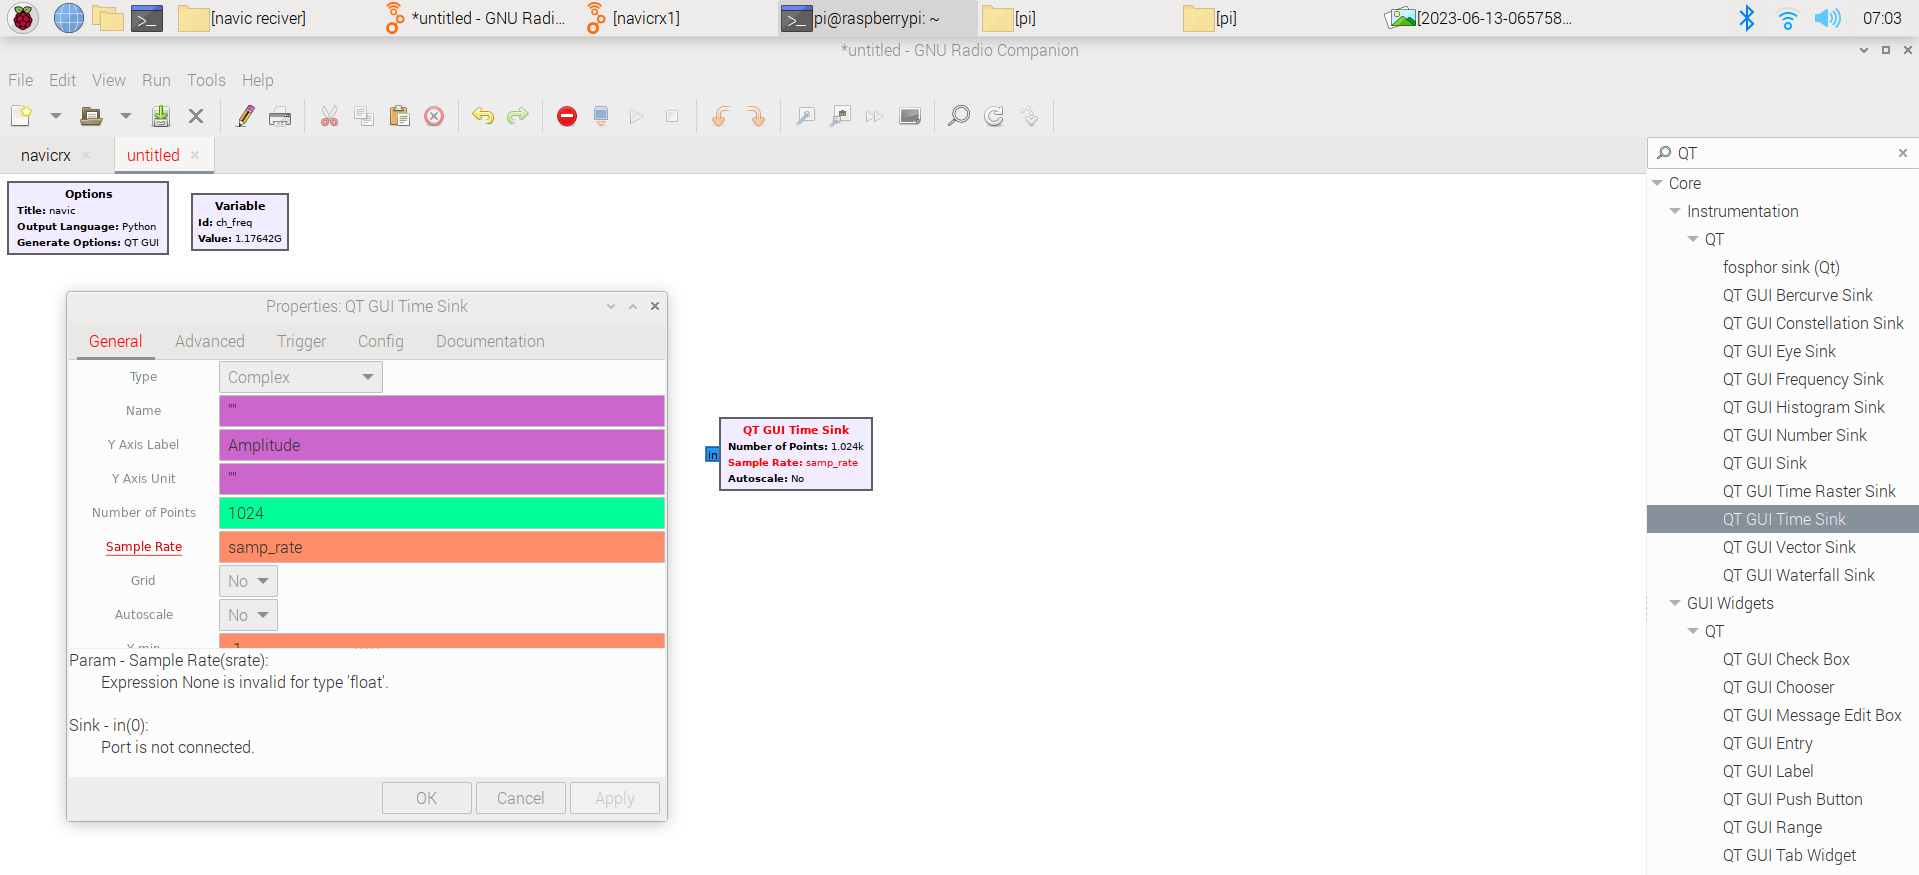
\includegraphics[width=\columnwidth]{figs/add.png}
\caption{Adding blocks}
\label{fig:adding blocks}
\end{figure}
\textbf{Step-2}:
Similarly do for USRP-Source block,complex to real ,complex to imaginary and QTGUI Time sink block.
\\
\textbf{Step-3}:
Change the parameters in each block according your values by double clicking on it.
\\
\textbf{Step-4}:
Connect them according to the flowgraph shown in \figref{fig:Rx_Block_diagram}.
\begin{figure}[H]
\centering
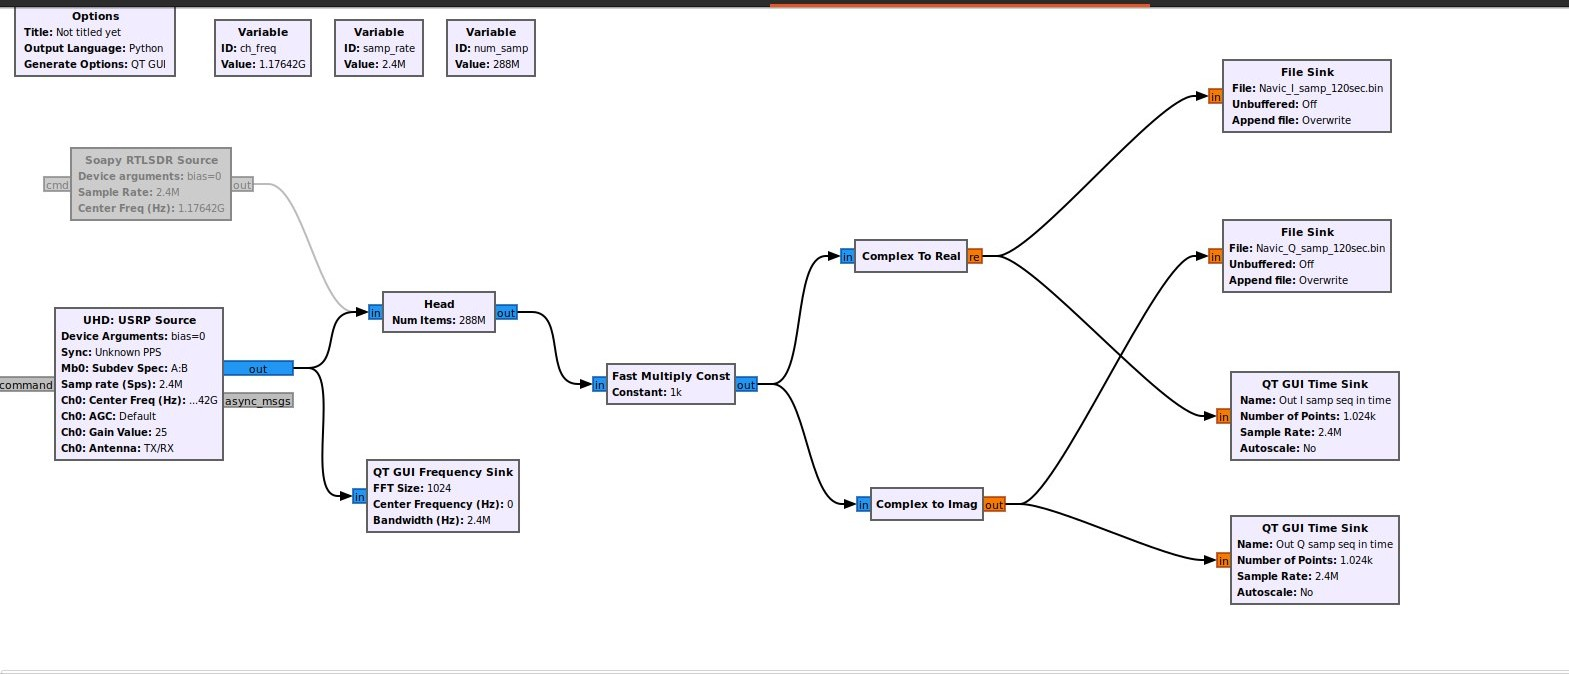
\includegraphics[width=\columnwidth]{figs/USRP_navic.jpg}
\caption{Block diagram of Receiver in GNU Radio}
\label{fig:Rx_Block_diagram_USRP}
\end{figure}
\textbf{Note}:
Refer the following website for any queries.
\begin{lstlisting}
https://wiki.gnuradio.org/index.php?title=Creating_Your_First_Block
\end{lstlisting}
 Explain each block in block diagram of Receiver.\\
	\solution \\
\textbf{1. RTL-SDR Source}:\\
The RTL-SDR Source block is used to stream samples from USRP-SDR device.
\begin{figure}[H]
\centering
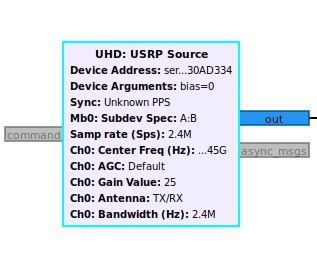
\includegraphics[width=0.4\columnwidth]{figs/usrp-sink.jpg}
\caption{USRP-SDR Source Block}
\label{fig:source block_USRP}
\end{figure}
Connect the USRP-SDR as shown flowgraph in \figref{fig:Rx_Block_diagram_USRP}.\\



\subsection{Results} 
\begin{figure}
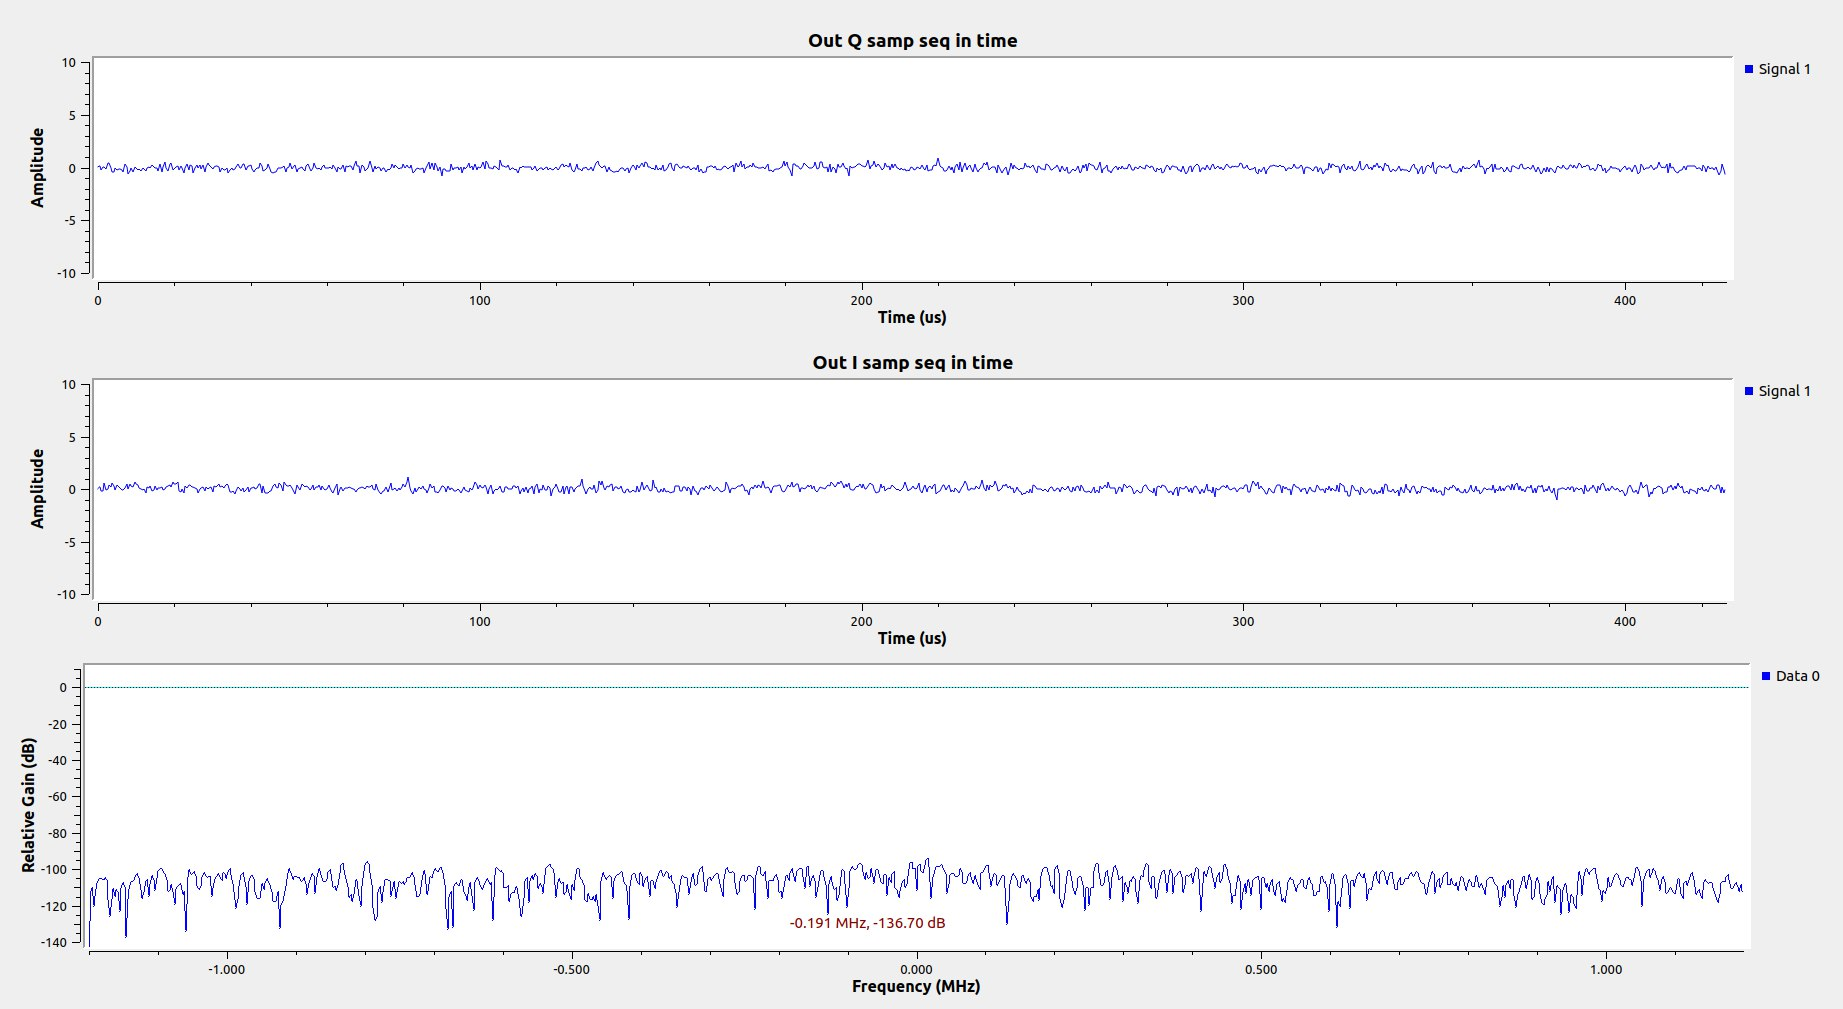
\includegraphics[width=0.8\columnwidth]{figs/USRP_results.jpg}
\caption{USRP receiver plots}
\label{fig:plots}
\end{figure}

I,Q samples will be stored in a file with .bin extension

Read the data from RTL SDR stored in .bin file using python code and without using GNU radio.
\\
\solution \\
The following code reads the data from RTL-SDR without GNU radio.
\begin{lstlisting}
codes/receiver/usrp_rx.py
\end{lstlisting}

















\chapter{Demodulation}
%\documentclass[onecolumn]{article}
%\usepackage{amsmath}
%\usepackage{enumerate}
%\usepackage{enumitem}
%\usepackage{listings}
%\usepackage[utf8]{inputenc}
%\usepackage{amssymb}
%\usepackage{tabularx}
%\usepackage{tikz}
%\usetikzlibrary{arrows,positioning,shapes.geometric}
%\usepackage{booktabs}
%\usepackage{multirow}
%\usepackage{siunitx}
%\usepackage{graphicx}
%\def\inputGnumericTable{}
%\usepackage{fullpage}
%\usepackage{color}
%\usepackage{array}
%\usepackage{longtable}
%\usepackage{calc}
%\usepackage{multirow}
%\usepackage{hhline}
%\usepackage{ifthen}
%\graphicspath{{./images/}}
%\usepackage[big]{titlesec}
%\usepackage{titlesec}

%%\titleformat*{\section}{\huge\bfseries}
%\titleformat*{\subsection}{\huge\bfseries}
%\titleformat*{\subsubsection}{\huge\bfseries}
%\lstset{
  %  frame=single,
  %  breaklines=true
%}
%\usepackage{hyperref}
%\usepackage[a3paper,outer=1.5cm,inner=1.5cm,top=1.75cm,bottom=1.5cm]{geometry}
%\def\mytitle{\textbf{DEMODULATION TECHNIQUES}}
%\def\myauthor{DUDEKULA USENI}
%\def\contact{r171099@rguktrkv.ac.in}

%\def\contact{r171099@rguktrkv.ac.in }
%\def\mymodule{Future Wireless Communication (FWC)}

%\thiswatermark{\centering \put(-15,-100.0){\includegraphics[scale=0.4]{iith.png}} }
%\title{\mytitle}
%\author{\myauthor\hspace{1em}\\\contact\ FWC22098 -\hspace{0.5em}IITH \hspace{0.5em}\mymodule\hspace{6em}}

%\providecommand{\mbf}{\mathbf}
%\newcommand{\myvec}[1]{\ensuremath{\begin{pmatrix}#1\end{pmatrix}}}
%\providecommand{\qfunc}[1]{\ensuremath{Q\left(#1\right)}}
%\providecommand{\cbrak}[1]{\ensuremath{\left\{#1\right\}}}
%\providecommand{\brak}[1]{\ensuremath{\left(#1\right)}}
%\providecommand{\lsbrak}[1]{\ensuremath{{}\left[#1\right.}}
%\providecommand{\rsbrak}[1]{\ensuremath{{}\left.#1\right]}}
%\providecommand{\rcbrak}[1]{\ensuremath{\left.#1\right\}}}
%\providecommand{\lcbrak}[1]{\ensuremath{\left\{#1\right.}}
%\providecommand{\sbrak}[1]{\ensuremath{{}\left[#1\right]}}

%\begin{document}
%%\begin{enumerate}
%\begin{Large}


\section{what is Demodulation}
%\item[\textbf{}] 

Demodulation is the process of extracting the original information or baseband signal from a modulated carrier signal.The purpose of demodulation is to retrieve the modulating signal, which could be analog or digital data, audio, video, or other forms of information. Demodulation is essential in various communication systems such as radio, television, cellular networks, and wireless data transmission.
%\end{Large}\\


The demodulation code used in NavIC may vary depending on the specific implementation and receiver hardware. However, I can provide you with a general outline of the demodulation process for NavIC signals.

NavIC signals are transmitted in the L5 frequency band (1176.45 MHz) using BPSK modulation for the navigation message and various modulation schemes (such as BOC and MBOC) for the ranging signal. The demodulation process typically involves the following steps:

\textbf{Signal Acquisition:} The receiver searches for and acquires the NavIC signal by correlating the received signal with a locally generated replica of the spreading code used by the satellites. This process helps in identifying the presence of the NavIC signal and estimating the initial timing offset.

\textbf{Carrier Tracking:} Once the signal is acquired, the receiver performs carrier tracking to estimate and track the carrier frequency and phase of the received signal. This is crucial for demodulation as it ensures accurate demodulation of the navigation message and ranging signal.

\textbf{Code Tracking:} The receiver performs code tracking to estimate and track the spreading code used by the satellites. This helps in maintaining synchronization with the transmitted signal and extracting the navigation data and ranging information.

\textbf{Data Extraction:} Once the demodulation is performed, the receiver extracts the navigation data from the demodulated signal. The navigation data includes information such as satellite ephemeris, clock correction, and other parameters necessary for calculating the receiver's position, velocity, and timing.

\subsection{Signal Acquistion}
\begin{normalsize}
\begin{figure}[!ht]%
\centering%
%\rule{30pt}{20pt}%
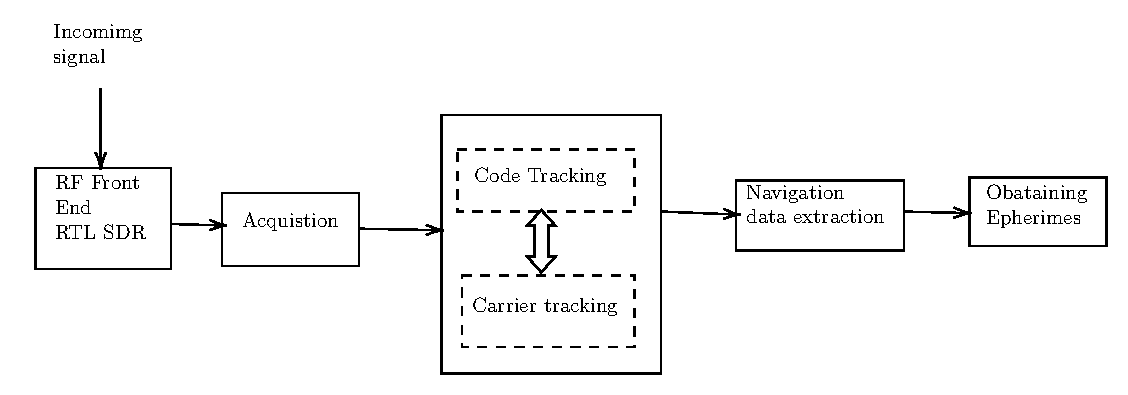
\includegraphics[scale=0.5]{figs/block2}
\end{figure} 

\end{normalsize}
\begin{center}
Figure2 : The Block Level Architecture in Demodulation
\end{center}
A generic IRNSS signal defined by its complex baseband equivalent, 
$S_T(t)$, the digital signal at the input of an Acquisition block can be written as:
\begin{align}
x_{IN}[k]=A(t)\hat S_T (t-\tau(t))e^{j(2 \pi f_D(t)t+\Phi))}\bigg|_{t=kT_s} +n(t)\bigg|_{t=kT_s}
\end{align}
%\end{Large}
\begin{table}[ht]
\centering
	\caption{\Large{Parameters Table in Signal Acquisition}}
	%%%%%%%%%%%%%%%%%%%%%%%%%%%%%%%%%%%%%%%%%%%%%%%%%%%%%%%%%%%%%%%%%%%%%%
%%                                                                  %%
%%  This is the header of a LaTeX2e file exported from Gnumeric.    %%
%%                                                                  %%
%%  This file can be compiled as it stands or included in another   %%
%%  LaTeX document. The table is based on the longtable package so  %%
%%  the longtable options (headers, footers...) can be set in the   %%
%%  preamble section below (see PRAMBLE).                           %%
%%                                                                  %%
%%  To include the file in another, the following two lines must be %%
%%  in the including file:                                          %%
%%        \def\inputGnumericTable{}                                 %%
%%  at the beginning of the file and:                               %%
%%        \input{name-of-this-file.tex}                             %%
%%  where the table is to be placed. Note also that the including   %%
%%  file must use the following packages for the table to be        %%
%%  rendered correctly:                                             %%
%%    \usepackage[latin1]{inputenc}                                 %%
%%    \usepackage{color}                                            %%
%%    \usepackage{array}                                            %%
%%    \usepackage{longtable}                                        %%
%%    \usepackage{calc}                                             %%
%%    \usepackage{multirow}                                         %%
%%    \usepackage{hhline}                                           %%
%%    \usepackage{ifthen}                                           %%
%%  optionally (for landscape tables embedded in another document): %%
%%    \usepackage{lscape}                                           %%
%%                                                                  %%
%%%%%%%%%%%%%%%%%%%%%%%%%%%%%%%%%%%%%%%%%%%%%%%%%%%%%%%%%%%%%%%%%%%%%%



%%  This section checks if we are begin input into another file or  %%
%%  the file will be compiled alone. First use a macro taken from   %%
%%  the TeXbook ex 7.7 (suggestion of Han-Wen Nienhuys).            %%
\def\ifundefined#1{\expandafter\ifx\csname#1\endcsname\relax}


%%  Check for the \def token for inputed files. If it is not        %%
%%  defined, the file will be processed as a standalone and the     %%
%%  preamble will be used.                                          %%
\ifundefined{inputGnumericTable}

%%  We must be able to close or not the document at the end.        %%
	\def\gnumericTableEnd{\end{document}}


%%%%%%%%%%%%%%%%%%%%%%%%%%%%%%%%%%%%%%%%%%%%%%%%%%%%%%%%%%%%%%%%%%%%%%
%%                                                                  %%
%%  This is the PREAMBLE. Change these values to get the right      %%
%%  paper size and other niceties.                                  %%
%%                                                                  %%
%%%%%%%%%%%%%%%%%%%%%%%%%%%%%%%%%%%%%%%%%%%%%%%%%%%%%%%%%%%%%%%%%%%%%%

	\documentclass[12pt%
			  %,landscape%
                    ]{report}
       \usepackage[latin1]{inputenc}
       \usepackage{fullpage}
       \usepackage{color}
       \usepackage{array}
       \usepackage{longtable}
       \usepackage{calc}
       \usepackage{multirow}
       \usepackage{hhline}
       \usepackage{ifthen}

	\begin{document}


%%  End of the preamble for the standalone. The next section is for %%
%%  documents which are included into other LaTeX2e files.          %%
\else

%%  We are not a stand alone document. For a regular table, we will %%
%%  have no preamble and only define the closing to mean nothing.   %%
    \def\gnumericTableEnd{}

%%  If we want landscape mode in an embedded document, comment out  %%
%%  the line above and uncomment the two below. The table will      %%
%%  begin on a new page and run in landscape mode.                  %%
%       \def\gnumericTableEnd{\end{landscape}}
%       \begin{landscape}


%%  End of the else clause for this file being \input.              %%
\fi

%%%%%%%%%%%%%%%%%%%%%%%%%%%%%%%%%%%%%%%%%%%%%%%%%%%%%%%%%%%%%%%%%%%%%%
%%                                                                  %%
%%  The rest is the gnumeric table, except for the closing          %%
%%  statement. Changes below will alter the table's appearance.     %%
%%                                                                  %%
%%%%%%%%%%%%%%%%%%%%%%%%%%%%%%%%%%%%%%%%%%%%%%%%%%%%%%%%%%%%%%%%%%%%%%

\providecommand{\gnumericmathit}[1]{#1} 
%%  Uncomment the next line if you would like your numbers to be in %%
%%  italics if they are italizised in the gnumeric table.           %%
%\renewcommand{\gnumericmathit}[1]{\mathit{#1}}
\providecommand{\gnumericPB}[1]%
{\let\gnumericTemp=\\#1\let\\=\gnumericTemp\hspace{0pt}}
 \ifundefined{gnumericTableWidthDefined}
        \newlength{\gnumericTableWidth}
        \newlength{\gnumericTableWidthComplete}
        \newlength{\gnumericMultiRowLength}
        \global\def\gnumericTableWidthDefined{}
 \fi
%% The following setting protects this code from babel shorthands.  %%
 \ifthenelse{\isundefined{\languageshorthands}}{}{\languageshorthands{english}}
%%  The default table format retains the relative column widths of  %%
%%  gnumeric. They can easily be changed to c, r or l. In that case %%
%%  you may want to comment out the next line and uncomment the one %%
%%  thereafter                                                      %%
\providecommand\gnumbox{\makebox[0pt]}
%%\providecommand\gnumbox[1][]{\makebox}

%% to adjust positions in multirow situations                       %%
\setlength{\bigstrutjot}{\jot}
\setlength{\extrarowheight}{\doublerulesep}

%%  The \setlongtables command keeps column widths the same across  %%
%%  pages. Simply comment out next line for varying column widths.  %%
\setlongtables

\setlength\gnumericTableWidth{%
	68pt+%
	235pt+%
0pt}
\def\gumericNumCols{2}
\setlength\gnumericTableWidthComplete{\gnumericTableWidth+%
         \tabcolsep*\gumericNumCols*2+\arrayrulewidth*\gumericNumCols}
\ifthenelse{\lengthtest{\gnumericTableWidthComplete > \linewidth}}%
         {\def\gnumericScale{\ratio{\linewidth-%
                        \tabcolsep*\gumericNumCols*2-%
                        \arrayrulewidth*\gumericNumCols}%
{\gnumericTableWidth}}}%
{\def\gnumericScale{1}}

%%%%%%%%%%%%%%%%%%%%%%%%%%%%%%%%%%%%%%%%%%%%%%%%%%%%%%%%%%%%%%%%%%%%%%
%%                                                                  %%
%% The following are the widths of the various columns. We are      %%
%% defining them here because then they are easier to change.       %%
%% Depending on the cell formats we may use them more than once.    %%
%%                                                                  %%
%%%%%%%%%%%%%%%%%%%%%%%%%%%%%%%%%%%%%%%%%%%%%%%%%%%%%%%%%%%%%%%%%%%%%%

\ifthenelse{\isundefined{\gnumericColA}}{\newlength{\gnumericColA}}{}\settowidth{\gnumericColA}{\begin{tabular}{@{}p{68pt*\gnumericScale}@{}}x\end{tabular}}
\ifthenelse{\isundefined{\gnumericColB}}{\newlength{\gnumericColB}}{}\settowidth{\gnumericColB}{\begin{tabular}{@{}p{235pt*\gnumericScale}@{}}x\end{tabular}}

\begin{longtable}[c]{%
	b{\gnumericColA}%
	b{\gnumericColB}%
	}

%%%%%%%%%%%%%%%%%%%%%%%%%%%%%%%%%%%%%%%%%%%%%%%%%%%%%%%%%%%%%%%%%%%%%%
%%  The longtable options. (Caption, headers... see Goosens, p.124) %%
%	\caption{The Table Caption.}             \\	%
% \hline	% Across the top of the table.
%%  The rest of these options are table rows which are placed on    %%
%%  the first, last or every page. Use \multicolumn if you want.    %%

%%  Header for the first page.                                      %%
%	\multicolumn{2}{c}{The First Header} \\ \hline 
%	\multicolumn{1}{c}{colTag}	%Column 1
%	&\multicolumn{1}{c}{colTag}	\\ \hline %Last column
%	\endfirsthead

%%  The running header definition.                                  %%
%	\hline
%	\multicolumn{2}{l}{\ldots\small\slshape continued} \\ \hline
%	\multicolumn{1}{c}{colTag}	%Column 1
%	&\multicolumn{1}{c}{colTag}	\\ \hline %Last column
%	\endhead

%%  The running footer definition.                                  %%
%	\hline
%	\multicolumn{2}{r}{\small\slshape continued\ldots} \\
%	\endfoot

%%  The ending footer definition.                                   %%
%	\multicolumn{2}{c}{That's all folks} \\ \hline 
%	\endlastfoot
%%%%%%%%%%%%%%%%%%%%%%%%%%%%%%%%%%%%%%%%%%%%%%%%%%%%%%%%%%%%%%%%%%%%%%

\hhline{|-|-}
	 \multicolumn{1}{|p{\gnumericColA}|}%
	{\gnumericPB{\raggedright}\gnumbox[l]{\hspace{0.75cm}\textbf{Symbol}}}
	&\multicolumn{1}{p{\gnumericColB}|}%
	{\gnumericPB{\raggedright}\gnumbox[l]{\hspace{3cm} \textbf{Definition}}}
\\
\hhline{|--|}
	 \multicolumn{1}{|p{\gnumericColA}|}%
	{\gnumericPB{\raggedright}\gnumbox[l]{\hspace{1cm}$x_{IN}[k]$}}
	&\multicolumn{1}{p{\gnumericColB}|}%
	{\gnumericPB{\raggedright}\gnumbox[l]{complex vector $I,Q$ samples of received signal}}
\\
\hhline{|--|}
	 \multicolumn{1}{|p{\gnumericColA}|}%
	{\gnumericPB{\raggedright}\gnumbox[l]{\hspace{1cm}A(t)}}
	&\multicolumn{1}{p{\gnumericColB}|}%
	{\gnumericPB{\raggedright}\gnumbox[l]{Signal Amplitude}}
\\
\hhline{|--|}
	 \multicolumn{1}{|p{\gnumericColA}|}%
	{\gnumericPB{\raggedright}\gnumbox[l]{\hspace{1cm}$\hat S_T(t)$}}
	&\multicolumn{1}{p{\gnumericColB}|}%
	{\gnumericPB{\raggedright}\gnumbox[l]{filtered version of $S_T(t)$}}
\\
\hhline{|--|}
	 \multicolumn{1}{|p{\gnumericColA}|}%
	{\gnumericPB{\raggedright}\gnumbox[l]{\hspace{1cm}$f_D(t)$ }}
	&\multicolumn{1}{p{\gnumericColB}|}%
	{\gnumericPB{\raggedright}\gnumbox[l]{Time - varing doppler shift}}
\\
\hhline{|--|}
	 \multicolumn{1}{|p{\gnumericColA}|}%
	{\gnumericPB{\raggedright}\gnumbox[l]{\hspace{1cm}$\Phi (t)$}}
	&\multicolumn{1}{p{\gnumericColB}|}%
	{\gnumericPB{\raggedright}\gnumbox[l]{Time - varing carrier phase shift}}
\\
\hhline{|--|}
	 \multicolumn{1}{|p{\gnumericColA}|}%
	{\gnumericPB{\raggedright}\gnumbox[l]{\hspace{1cm}n(t) }}
	&\multicolumn{1}{p{\gnumericColB}|}%
	{\gnumericPB{\raggedright}\gnumbox[l]{Term modelling random noise}}
\\
\hhline{|--|}
	 \multicolumn{1}{|p{\gnumericColA}|}%
	{\gnumericPB{\raggedright}\gnumbox[l]{\hspace{1cm}$T_s$ }}
	&\multicolumn{1}{p{\gnumericColB}|}%
	{\gnumericPB{\raggedright}\gnumbox[l]{sampling period}}
\\
\hhline{|-|-|}
\end{longtable}

\ifthenelse{\isundefined{\languageshorthands}}{}{\languageshorthands{\languagename}}
\gnumericTableEnd

\end{table}
%\begin{Large}



\subsubsection{Implementation of CA PCPS Acquisition}
The Parallel Code Phase Search (PCPS) algorithm is described as follows:
Input signal buffer $x_{IN}$ of k complex samples, acquisition threshold $\gamma$\\
provided by the Signal Conditioner; on-memory FFT of the local replica,
\begin{align}
D[k]=FFT_k\{d[k]\}
\end{align}
\begin{align}
\text{input signal power estimation :} \hat P_{in} = \frac{1}{k}\sum_{k=0}^{k-1} \big| x_{IN}[k]\big| ^2
\end{align}
\begin{align}
\check f_D=[ f_{min}, f_{max}]\hspace{0.5cm} in \hspace{0.5cm}f_{steps} 
\end{align}
\begin{align}
\text{carrier wipe off:}\hspace{0.5cm}x[k]=x_{IN}[k]e^{-(j2 \pi \check f_D k T_s)},\hspace{0.5cm}for\hspace{0.5cm}k=0,...,k-1
\end{align}
\begin{align}
X[k]=FFT_k\{x[k]\}
\end{align}
\begin{align}
Y[k]=X[k].D[k],\hspace{0.5cm} for k=0,...k-1. 
\end{align}

\begin{align}
R_{xd}(\check f_D,\tau) = \frac{1}{k^2}IFFT_k\{Y[k]\}
\end{align}

Search maximum and its indices in the search grid:
\begin{align}
\{S_{max},f_i,\tau_j\} = max_{f,\tau} \big |R_{xd}(f,\tau)\big | ^2
\end{align}
Compute the Generalized Likelihood Ratio Test (GLRT) function with normalized variance:
\begin{align}
\Gamma_{GLRT} = \frac{2kS_{max}}{\hat P_{in}}
\end{align}
if $\Gamma_{GLRT} > \gamma$\\
Declare positive acquisition and provides coarse estimation of code phase $\hat \tau_{acq} = \tau_j $and Doppler shift $\hat f_{D_{acq}}=f_i$,\\
other wise declare negative acquisition.

%\end{Large}
The acquisition results are generated using the below code\\
\textbf{Code}
\begin{lstlisting}
code/e2e_sim/main.ipynb
\end{lstlisting}
\textbf{Result}
\begin{lstlisting}
Acquisition results for PRN ID 5
 Status:True Doppler:3500 Delay/Code-Phase:300/30.0
Acquisition results for PRN ID 7
 Status:True Doppler:2500 Delay/Code-Phase:587/58.7
Acquisition results for PRN ID 3
 Status:True Doppler:1500 Delay/Code-Phase:426/42.6
Acquisition results for PRN ID 1
 Status:True Doppler:2500 Delay/Code-Phase:313/31.3
\end{lstlisting}


\subsection{Carrier tracking loop:}

\textbf{Phase locked loop(PLL)}\\
The carrier loop discriminator defines the type of tracking loop as a PLL, aCostas PLL (which is a PLL-type discriminator that tolerates the presence of data modulation on the baseband signal), or a frequency lock loop (FLL).Carrier tracking loop tracks the frequency and phase of the received signal by detecting the phase error between replicated signal and incoming signal and accordingly replicated signal produced by numerically controlled oscillator (NCO) is adjusted to synchronize with incoming signal in both frequency and phase. For zero phase error detected, navigation data is accurately extracted. 
%\begin{normalsize}
\begin{figure}[!ht]%
%\centering%
%\rule{30pt}{20pt}%
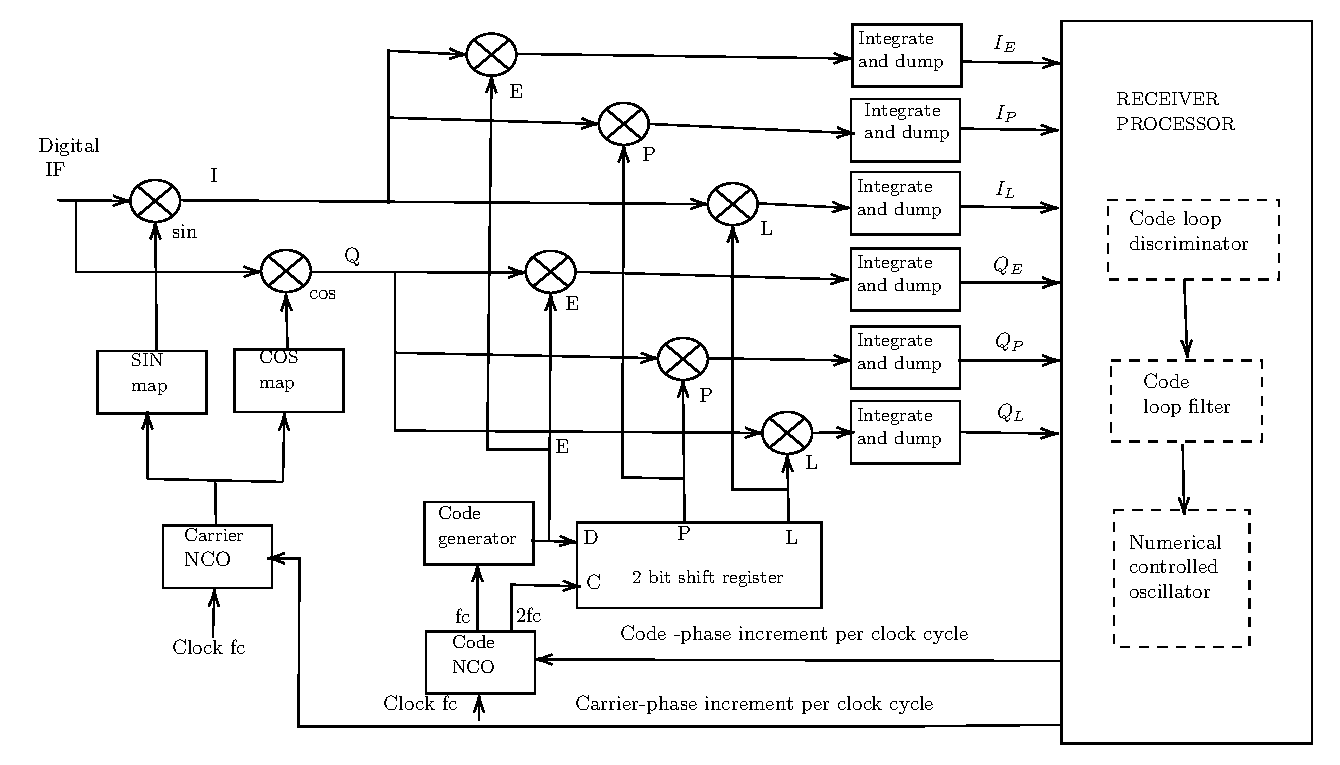
\includegraphics[scale=0.5]{figs/block3}
\end{figure}
%\end{normalsize}
%\begin{Large}
\begin{center}
Figure3 : Generic digital receiver channel
\end{center}
\begin{align}
\text{PLL Discriminator} =ATAN2(I_P,Q_P) = \tan^{-1}\brak{\frac{I_P}{Q_P}}
\end{align}
compares the phase error outputs of these PLL discriminators assuming no noise in the I and Q signals. Note that the ATAN2 discriminator is the only one that remains linear over the full input error range of $\pm180^{\circ}$. However, in the presence of noise, both of the discriminator outputs are linear only near the $0^{\circ}$ region. These PLL discriminators will achieve the 6-dB improvement in signal tracking threshold (by comparison with the Costas discriminators described next) for the dataless carrier because they track the full four quadrant range of the input signal.\\
\textbf{Frequency locked loop}\\
PLLs replicate the exact phase and frequency of the incoming SV (converted to IF) to perform the carrier wipeoff function. FLLs perform the carrier wipeoff process by replicating the approximate frequency, and they typically permit the phase to rotate with respect to the incoming carrier signal.
\begin{align}
\text{FLL Discriminator} =\frac{ATAN2(dot,cross)}{t2-t1}
\end{align}
ATAN2(dot, cross)FLL discriminators are equal to half the predetection bandwidths. The (cross)$\times$ sign(dot) FLL discriminator frequency pull-in ranges are only one-fourth of the predetection bandwidths. Also note that the (cross) $\times$ sign(dot) and the cross FLL discriminator outputs, whose outputs are sine functions divided by the sample time interval $(t_2 -t _1)$ in seconds, are also divided by 4 to more accurately approximate the true input frequency error. The ATAN2 (x, y) function returns the answer in radians, is converted to degrees, divided by the sample time interval $(t_2 - t_1)$in seconds,
and is also divided by 360 to produce at its output a true representation of the input
frequency error within its pull-in range
\subsection{Code tracking loop:}
\textbf{Delay locked loop}
Post the carrier signal synchronization, received CA code samples is synchronized by aligning with replicated CA code samples by shifting right or left. To determine the direction of shift, the I and Q outputs are multiplied with prompt code (PRN code which is phase aligned), early code (prompt PRN code shifted by some samples to the right) and late code (prompt PRN code shifted by some samples to the left) resulting in corresponding to I and Q channel respectively.IRNSS receiver delay lock loop (DLL) discriminators and their characteristics.

 \begin{align}
 E=\sqrt[]{I_{ES}^2+Q_{ES}^2}
 \end{align}
 \begin{align}
 L=\sqrt[]{I_{LS}^2+Q_{LS}^2}
 \end{align}
\begin{align}
\text{DLL Discriminator} (\epsilon)=\frac{1}{2}\frac{E-L}{E+L}
\end{align}
Noncoherent early minus late envelope normalized by $E + L$ to remove amplitude sensitivity High computational load.For  1-chip $E - L$ correlator spacing, produces true tracking error within $\pm 0.5$  chip of input error (in the absence of noise).
Becomes unstable (divide by zero) at $\pm 1.5$ -chip input error, but this is well beyond code tracking threshold in the presence of noise.
%\end{Large}\\
\subsection{Loop filter characteristics}
\begin{table}[ht]
\centering
	\caption{\Large{Loop order filters }}
	%%%%%%%%%%%%%%%%%%%%%%%%%%%%%%%%%%%%%%%%%%%%%%%%%%%%%%%%%%%%%%%%%%%%%%
%%                                                                  %%
%%  This is the header of a LaTeX2e file exported from Gnumeric.    %%
%%                                                                  %%
%%  This file can be compiled as it stands or included in another   %%
%%  LaTeX document. The table is based on the longtable package so  %%
%%  the longtable options (headers, footers...) can be set in the   %%
%%  preamble section below (see PRAMBLE).                           %%
%%                                                                  %%
%%  To include the file in another, the following two lines must be %%
%%  in the including file:                                          %%
%%        \def\inputGnumericTable{}                                 %%
%%  at the beginning of the file and:                               %%
%%        \input{name-of-this-file.tex}                             %%
%%  where the table is to be placed. Note also that the including   %%
%%  file must use the following packages for the table to be        %%
%%  rendered correctly:                                             %%
%%    \usepackage[latin1]{inputenc}                                 %%
%%    \usepackage{color}                                            %%
%%    \usepackage{array}                                            %%
%%    \usepackage{longtable}                                        %%
%%    \usepackage{calc}                                             %%
%%    \usepackage{multirow}                                         %%
%%    \usepackage{hhline}                                           %%
%%    \usepackage{ifthen}                                           %%
%%  optionally (for landscape tables embedded in another document): %%
%%    \usepackage{lscape}                                           %%
%%                                                                  %%
%%%%%%%%%%%%%%%%%%%%%%%%%%%%%%%%%%%%%%%%%%%%%%%%%%%%%%%%%%%%%%%%%%%%%%



%%  This section checks if we are begin input into another file or  %%
%%  the file will be compiled alone. First use a macro taken from   %%
%%  the TeXbook ex 7.7 (suggestion of Han-Wen Nienhuys).            %%
\def\ifundefined#1{\expandafter\ifx\csname#1\endcsname\relax}


%%  Check for the \def token for inputed files. If it is not        %%
%%  defined, the file will be processed as a standalone and the     %%
%%  preamble will be used.                                          %%
\ifundefined{inputGnumericTable}

%%  We must be able to close or not the document at the end.        %%
	\def\gnumericTableEnd{\end{document}}


%%%%%%%%%%%%%%%%%%%%%%%%%%%%%%%%%%%%%%%%%%%%%%%%%%%%%%%%%%%%%%%%%%%%%%
%%                                                                  %%
%%  This is the PREAMBLE. Change these values to get the right      %%
%%  paper size and other niceties.                                  %%
%%                                                                  %%
%%%%%%%%%%%%%%%%%%%%%%%%%%%%%%%%%%%%%%%%%%%%%%%%%%%%%%%%%%%%%%%%%%%%%%

	\documentclass[12pt%
			  %,landscape%
                    ]{report}
       \usepackage[latin1]{inputenc}
       \usepackage{fullpage}
       \usepackage{color}
       \usepackage{array}
       \usepackage{longtable}
       \usepackage{calc}
       \usepackage{multirow}
       \usepackage{hhline}
       \usepackage{ifthen}

	\begin{document}


%%  End of the preamble for the standalone. The next section is for %%
%%  documents which are included into other LaTeX2e files.          %%
\else

%%  We are not a stand alone document. For a regular table, we will %%
%%  have no preamble and only define the closing to mean nothing.   %%
    \def\gnumericTableEnd{}

%%  If we want landscape mode in an embedded document, comment out  %%
%%  the line above and uncomment the two below. The table will      %%
%%  begin on a new page and run in landscape mode.                  %%
%       \def\gnumericTableEnd{\end{landscape}}
%       \begin{landscape}


%%  End of the else clause for this file being \input.              %%
\fi

%%%%%%%%%%%%%%%%%%%%%%%%%%%%%%%%%%%%%%%%%%%%%%%%%%%%%%%%%%%%%%%%%%%%%%
%%                                                                  %%
%%  The rest is the gnumeric table, except for the closing          %%
%%  statement. Changes below will alter the table's appearance.     %%
%%                                                                  %%
%%%%%%%%%%%%%%%%%%%%%%%%%%%%%%%%%%%%%%%%%%%%%%%%%%%%%%%%%%%%%%%%%%%%%%

\providecommand{\gnumericmathit}[1]{#1} 
%%  Uncomment the next line if you would like your numbers to be in %%
%%  italics if they are italizised in the gnumeric table.           %%
%\renewcommand{\gnumericmathit}[1]{\mathit{#1}}
\providecommand{\gnumericPB}[1]%
{\let\gnumericTemp=\\#1\let\\=\gnumericTemp\hspace{0pt}}
 \ifundefined{gnumericTableWidthDefined}
        \newlength{\gnumericTableWidth}
        \newlength{\gnumericTableWidthComplete}
        \newlength{\gnumericMultiRowLength}
        \global\def\gnumericTableWidthDefined{}
 \fi
%% The following setting protects this code from babel shorthands.  %%
 \ifthenelse{\isundefined{\languageshorthands}}{}{\languageshorthands{english}}
%%  The default table format retains the relative column widths of  %%
%%  gnumeric. They can easily be changed to c, r or l. In that case %%
%%  you may want to comment out the next line and uncomment the one %%
%%  thereafter                                                      %%
\providecommand\gnumbox{\makebox[0pt]}
%%\providecommand\gnumbox[1][]{\makebox}

%% to adjust positions in multirow situations                       %%
\setlength{\bigstrutjot}{\jot}
\setlength{\extrarowheight}{\doublerulesep}

%%  The \setlongtables command keeps column widths the same across  %%
%%  pages. Simply comment out next line for varying column widths.  %%
\setlongtables

\setlength\gnumericTableWidth{%
	70pt+%
	100pt+%
	80pt+%
0pt}
\def\gumericNumCols{3}
\setlength\gnumericTableWidthComplete{\gnumericTableWidth+%
         \tabcolsep*\gumericNumCols*2+\arrayrulewidth*\gumericNumCols}
\ifthenelse{\lengthtest{\gnumericTableWidthComplete > \linewidth}}%
         {\def\gnumericScale{\ratio{\linewidth-%
                        \tabcolsep*\gumericNumCols*2-%
                        \arrayrulewidth*\gumericNumCols}%
{\gnumericTableWidth}}}%
{\def\gnumericScale{1}}

%%%%%%%%%%%%%%%%%%%%%%%%%%%%%%%%%%%%%%%%%%%%%%%%%%%%%%%%%%%%%%%%%%%%%%
%%                                                                  %%
%% The following are the widths of the various columns. We are      %%
%% defining them here because then they are easier to change.       %%
%% Depending on the cell formats we may use them more than once.    %%
%%                                                                  %%
%%%%%%%%%%%%%%%%%%%%%%%%%%%%%%%%%%%%%%%%%%%%%%%%%%%%%%%%%%%%%%%%%%%%%%

\ifthenelse{\isundefined{\gnumericColA}}{\newlength{\gnumericColA}}{}\settowidth{\gnumericColA}{\begin{tabular}{@{}p{70pt*\gnumericScale}@{}}x\end{tabular}}
\ifthenelse{\isundefined{\gnumericColB}}{\newlength{\gnumericColB}}{}\settowidth{\gnumericColB}{\begin{tabular}{@{}p{100pt*\gnumericScale}@{}}x\end{tabular}}
\ifthenelse{\isundefined{\gnumericColC}}{\newlength{\gnumericColC}}{}\settowidth{\gnumericColC}{\begin{tabular}{@{}p{80pt*\gnumericScale}@{}}x\end{tabular}}

\begin{longtable}[c]{%
	b{\gnumericColA}%
	b{\gnumericColB}%
	b{\gnumericColC}%
	}

%%%%%%%%%%%%%%%%%%%%%%%%%%%%%%%%%%%%%%%%%%%%%%%%%%%%%%%%%%%%%%%%%%%%%%
%%  The longtable options. (Caption, headers... see Goosens, p.124) %%
%	\caption{The Table Caption.}             \\	%
% \hline	% Across the top of the table.
%%  The rest of these options are table rows which are placed on    %%
%%  the first, last or every page. Use \multicolumn if you want.    %%

%%  Header for the first page.                                      %%
%	\multicolumn{3}{c}{The First Header} \\ \hline 
%	\multicolumn{1}{c}{colTag}	%Column 1
%	&\multicolumn{1}{c}{colTag}	%Column 2
%	&\multicolumn{1}{c}{colTag}	\\ \hline %Last column
%	\endfirsthead

%%  The running header definition.                                  %%
%	\hline
%	\multicolumn{3}{l}{\ldots\small\slshape continued} \\ \hline
%	\multicolumn{1}{c}{colTag}	%Column 1
%	&\multicolumn{1}{c}{colTag}	%Column 2
%	&\multicolumn{1}{c}{colTag}	\\ \hline %Last column
%	\endhead

%%  The running footer definition.                                  %%
%	\hline
%	\multicolumn{3}{r}{\small\slshape continued\ldots} \\
%	\endfoot

%%  The ending footer definition.                                   %%
%	\multicolumn{3}{c}{That's all folks} \\ \hline 
%	\endlastfoot
%%%%%%%%%%%%%%%%%%%%%%%%%%%%%%%%%%%%%%%%%%%%%%%%%%%%%%%%%%%%%%%%%%%%%%

\hhline{|-|-|-}
	 \multicolumn{1}{|p{\gnumericColA}|}%
	{\gnumericPB{\raggedright}\gnumbox[l]{\textbf{Loop Order}}}
	&\multicolumn{1}{p{\gnumericColB}|}%
	{\gnumericPB{\raggedright}\gnumbox[l]{\textbf{Noise Bandwidth}}}
	&\multicolumn{1}{p{\gnumericColC}|}%
	{\gnumericPB{\raggedright}\gnumbox[l]{\textbf{Typical Filter  }}}
\\
%\hhline{|---|}
	 \multicolumn{1}{|p{\gnumericColA}|}%
	{\gnumericPB{\raggedleft}\gnumbox[r]{}}
	&\multicolumn{1}{p{\gnumericColB}|}%
	{\gnumericPB{\raggedright}\gnumbox[l]{\textbf{$ B_n$ (Hz)}}}
	&\multicolumn{1}{p{\gnumericColC}|}%
	{\gnumericPB{\raggedright}\gnumbox[l]{\textbf{ Values }}}
	%{\gnumericPB{\raggedright}\gnumbox[l]{}}\\
	\\
\hhline{|---|}
	 \multicolumn{1}{|p{\gnumericColA}|}%
	{\gnumericPB{\raggedleft}\gnumbox[r]{First}}
	&\multicolumn{1}{p{\gnumericColB}|}%
	{\gnumericPB{\raggedright}\gnumbox[l]{\hspace{0.5cm}$\frac{\omega_o}{4}$}}
	&\multicolumn{1}{p{\gnumericColC}|}%
	{\gnumericPB{\raggedright}\gnumbox[l]{\hspace{0.5cm}$\omega_o $ }}
	%{\gnumericPB{\raggedright}\gnumbox[l]{}}\\
	\\
%\hhline{|---|}
	 \multicolumn{1}{|p{\gnumericColA}|}%
	{\gnumericPB{\raggedleft}\gnumbox[r]{}}
	&\multicolumn{1}{p{\gnumericColB}|}%
	{\gnumericPB{\raggedright}\gnumbox[l]{}}
	&\multicolumn{1}{p{\gnumericColC}|}%
	{\gnumericPB{\raggedright}\gnumbox[l]{ $B_n=0.25\omega_o$}}
\\
\hhline{|---|}
\multicolumn{1}{|p{\gnumericColA}|}%
	{\gnumericPB{\raggedleft}\gnumbox[r]{}}
	&\multicolumn{1}{p{\gnumericColB}|}%
	{\gnumericPB{\raggedright}\gnumbox[l]{}}
	&\multicolumn{1}{p{\gnumericColC}|}%
	{\gnumericPB{\raggedright}\gnumbox[l]{ $\omega_o^2$}}
	 
\\
%\hhline{|---|}
	\multicolumn{1}{|p{\gnumericColA}|}%
	{\gnumericPB{\raggedleft}\gnumbox[r]{Second}}
	&\multicolumn{1}{p{\gnumericColB}|}%
	{\gnumericPB{\raggedright}\gnumbox[l]{$\frac{\omega(1+a_2^2)}{4a_2}$}}
	&\multicolumn{1}{p{\gnumericColC}|}%
	{\gnumericPB{\raggedright}\gnumbox[l]{$a_2\omega_o=1.414\omega_o$}}
\\
%\hhline{|-|-|-|}
\multicolumn{1}{|p{\gnumericColA}|}%
	{\gnumericPB{\raggedleft}\gnumbox[r]{}}
	&\multicolumn{1}{p{\gnumericColB}|}%
	{\gnumericPB{\raggedright}\gnumbox[l]{}}
	&\multicolumn{1}{p{\gnumericColC}|}%
	{\gnumericPB{\raggedright}\gnumbox[l]{ $B_n=0.53\omega_o$}}
	
	\\
\hhline{|-|-|-|}
 \multicolumn{1}{|p{\gnumericColA}|}%
	{\gnumericPB{\raggedleft}\gnumbox[r]{}}
	&\multicolumn{1}{p{\gnumericColB}|}%
	{\gnumericPB{\raggedright}\gnumbox[l]{}}
	&\multicolumn{1}{p{\gnumericColC}|}%
	{\gnumericPB{\raggedright}\gnumbox[l]{$\omega_o^3$ }}
		\\
%\hhline{|-|-|-|}
 \multicolumn{1}{|p{\gnumericColA}|}%
	{\gnumericPB{\raggedleft}\gnumbox[r]{Third}}
	&\multicolumn{1}{p{\gnumericColB}|}%
	{\gnumericPB{\raggedright}\gnumbox[l]{$\frac{\omega(a_3b_3^2+a_3^2-b_3)}{4(a_3b_3-1)}$}}
	&\multicolumn{1}{p{\gnumericColC}|}%
	{\gnumericPB{\raggedright}\gnumbox[l]{$ a_3\omega_o^2=1.1\omega_o^2$}}
	\\
%\hhline{|-|-|-|}
 \multicolumn{1}{|p{\gnumericColA}|}%
	{\gnumericPB{\raggedleft}\gnumbox[r]{}}
	&\multicolumn{1}{p{\gnumericColB}|}%
	{\gnumericPB{\raggedright}\gnumbox[l]{}}
	&\multicolumn{1}{p{\gnumericColC}|}%
	{\gnumericPB{\raggedright}\gnumbox[l]{$b_3\omega_o=2.4\omega_o$}}
	\\
%\hhline{|-|-|-|}
 \multicolumn{1}{|p{\gnumericColA}|}%
	{\gnumericPB{\raggedleft}\gnumbox[r]{}}
	&\multicolumn{1}{p{\gnumericColB}|}%
	{\gnumericPB{\raggedright}\gnumbox[l]{}}
	&\multicolumn{1}{p{\gnumericColC}|}%
	{\gnumericPB{\raggedright}\gnumbox[l]{ $B_n=0.7845\omega_o$}}
		\\
\hhline{|-|-|-|}
 
\end{longtable}

\ifthenelse{\isundefined{\languageshorthands}}{}{\languageshorthands{\languagename}}
\gnumericTableEnd

\end{table}

The values for the second-order coefficient $a_2$ and third-order coefficients $a_3$ and $b_3$ can be determined from Table 3. These coefficients are the same for FLL, PLL, or DLL applications if the loop
order and the noise bandwidth,$B_n$ , are the same.Note that the FLL coefficient insertion point into the filter is one integrator back from the PLL and DLL insertion points.This is because the FLL error is in units of hertz (change in range per unit of time).\\
The tracking results are generated using the below code\\
\textbf{Code}
\begin{lstlisting}
code/e2e_sim/main_ipynb
\end{lstlisting}
\textbf{Result}
\begin{lstlisting}
Tracking result for PRN ID:5
Transmitted Bits:
 [0. 1. 0. 1. 0. 0. 0. 1. 0. 1. 1. 0. 0. 0. 1. 1. 1. 0. 0. 1. 1. 1. 1. 0.1. 0. 1. 1. 0. 1. 0. 0. 1. 0. 0. 0. 1. 0. 1. 1. 1. 0. 1. 1. 0. 0. 1. 0. 0. 0.]
Received bits:
 [1. 1. 0. 1. 0. 1. 1. 1. 0. 1. 0. 0. 1. 1. 1. 0. 0. 0. 1. 1. 0. 0. 0. 0.1. 0. 1. 0. 0. 1. 0. 1. 1. 0. 1. 1. 1. 0. 1. 0. 0. 0. 1. 0. 0. 1. 1. 0.1. 1.]
Received bits inverted:
 [0. 0. 1. 0. 1. 0. 0. 0. 1. 0. 1. 1. 0. 0. 0. 1. 1. 1. 0. 0. 1. 1. 1. 1.0. 1. 0. 1. 1. 0. 1. 0. 0. 1. 0. 0. 0. 1. 0. 1. 1. 1. 0. 1. 1. 0. 0. 1. 0. 0.]
\end{lstlisting}

\begin{figure}[ht]
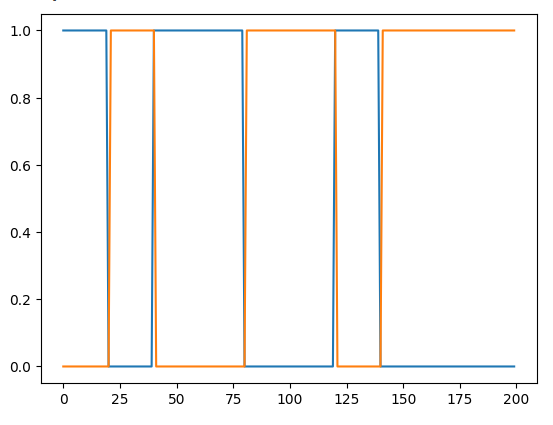
\includegraphics[width=0.5\columnwidth]{figs/tracking_plot.png}
\caption{tracking result plot}
\end{figure}

The functions for acquisition and tracking are present in the below code
\begin{lstlisting}
codes/demodulation/demodulation.py
\end{lstlisting}


%\end{Large}

%\end{enumerate}
%\end{document}

\chapter{Channel Decoding}
\section{Definition}
Channel decoding in NAVIC, the Indian Regional Navigation Satellite System, involves the process of error correction and retrieval of the original data transmitted over the satellite link. The channel decoding scheme used in NAVIC is based on a convolutional coding technique known as Rate 1/2 Convolutional Code with Viterbi decoding.
\subsection{Process}
Here is a high-level description of the channel decoding process in NAVIC:
\begin{figure}[h!]
	\centering
	%\subimport{table/}{table1.tex}
	

\tikzset{every picture/.style={line width=0.75pt}} %set default line width to 0.75pt        

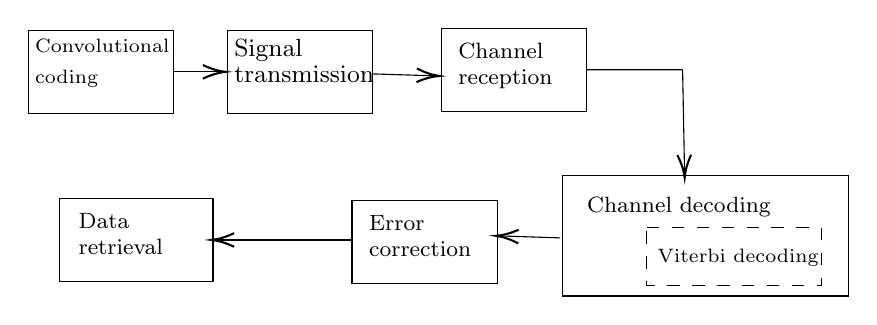
\begin{tikzpicture}[x=0.75pt,y=0.75pt,yscale=-1,xscale=1]
%uncomment if require: \path (0,300); %set diagram left start at 0, and has height of 300

%Shape: Rectangle [id:dp5040039695529985] 
\draw   (24,91) -- (94,91) -- (94,131) -- (24,131) -- cycle ;
%Straight Lines [id:da6707039679717985] 
\draw    (94.09,111.01) -- (117.09,111.01) ;
\draw [shift={(119.09,111.01)}, rotate = 180] [color={rgb, 255:red, 0; green, 0; blue, 0 }  ][line width=0.75]    (10.93,-3.29) .. controls (6.95,-1.4) and (3.31,-0.3) .. (0,0) .. controls (3.31,0.3) and (6.95,1.4) .. (10.93,3.29)   ;
%Shape: Rectangle [id:dp6676087786831228] 
\draw   (120,91) -- (190,91) -- (190,131) -- (120,131) -- cycle ;
%Shape: Rectangle [id:dp12552727666705787] 
\draw   (223,90) -- (293,90) -- (293,130) -- (223,130) -- cycle ;
%Shape: Rectangle [id:dp041785178904101716] 
\draw   (281.27,161.01) -- (419.27,161.01) -- (419.27,219.01) -- (281.27,219.01) -- cycle ;
%Shape: Rectangle [id:dp3930533301018766] 
\draw   (180,173) -- (250,173) -- (250,213) -- (180,213) -- cycle ;
%Shape: Rectangle [id:dp6457667866806436] 
\draw   (39.09,172) -- (113,172) -- (113,212) -- (39.09,212) -- cycle ;
%Straight Lines [id:da408023078866502] 
\draw    (190.09,112.01) -- (220.09,112.94) ;
\draw [shift={(222.09,113.01)}, rotate = 181.79] [color={rgb, 255:red, 0; green, 0; blue, 0 }  ][line width=0.75]    (10.93,-3.29) .. controls (6.95,-1.4) and (3.31,-0.3) .. (0,0) .. controls (3.31,0.3) and (6.95,1.4) .. (10.93,3.29)   ;
%Straight Lines [id:da20565488006754173] 
\draw    (339.27,110.01) -- (340.23,160.01) ;
\draw [shift={(340.27,162.01)}, rotate = 268.9] [color={rgb, 255:red, 0; green, 0; blue, 0 }  ][line width=0.75]    (10.93,-3.29) .. controls (6.95,-1.4) and (3.31,-0.3) .. (0,0) .. controls (3.31,0.3) and (6.95,1.4) .. (10.93,3.29)   ;
%Straight Lines [id:da606104691567432] 
\draw    (293,110) -- (339.27,110.01) ;
%Straight Lines [id:da9255999705919356] 
\draw    (280.27,191.01) -- (251.27,190.07) ;
\draw [shift={(249.27,190.01)}, rotate = 1.85] [color={rgb, 255:red, 0; green, 0; blue, 0 }  ][line width=0.75]    (10.93,-3.29) .. controls (6.95,-1.4) and (3.31,-0.3) .. (0,0) .. controls (3.31,0.3) and (6.95,1.4) .. (10.93,3.29)   ;
%Straight Lines [id:da848136557718163] 
\draw    (180.27,192.01) -- (114.27,192.01) ;
\draw [shift={(112.27,192.01)}, rotate = 360] [color={rgb, 255:red, 0; green, 0; blue, 0 }  ][line width=0.75]    (10.93,-3.29) .. controls (6.95,-1.4) and (3.31,-0.3) .. (0,0) .. controls (3.31,0.3) and (6.95,1.4) .. (10.93,3.29)   ;
%Shape: Rectangle [id:dp6659957800064993] 
\draw  [dash pattern={on 4.5pt off 4.5pt}] (322.09,186.01) -- (406,186.01) -- (406,214) -- (322.09,214) -- cycle ;

% Text Node
\draw (26,94) node [anchor=north west][inner sep=0.75pt]  [font=\small] [align=left] {{\scriptsize Convolutional}\\{\scriptsize coding}};
% Text Node
\draw (122,94) node [anchor=north west][inner sep=0.75pt]  [font=\footnotesize] [align=left] {{\small Signal }\\{\small transmission}};
% Text Node
\draw (230,96) node [anchor=north west][inner sep=0.75pt]  [font=\footnotesize] [align=left] {Channel \\reception};
% Text Node
\draw (326,195) node [anchor=north west][inner sep=0.75pt]  [font=\scriptsize] [align=left] {Viterbi decoding};
% Text Node
\draw (292,170) node [anchor=north west][inner sep=0.75pt]  [font=\footnotesize] [align=left] {Channel decoding};
% Text Node
\draw (187,179) node [anchor=north west][inner sep=0.75pt]  [font=\footnotesize] [align=left] {Error \\correction};
% Text Node
\draw (47,178) node [anchor=north west][inner sep=0.75pt]  [font=\footnotesize] [align=left] {Data\\retrieval};


\end{tikzpicture}


	\caption{The Block Level Architecture in Channel Decoding}
	\label{figs:decoderBlock}
	\end{figure}


\subsection{Convolutional Code Representation:}

The convolutional code is represented as a state diagram or trellis, where each state represents a unique history of the encoded bits.
The trellis consists of nodes and branches. Nodes correspond to states, and branches represent transitions between states.
Each branch is labeled with the input bit and the encoded output bits associated with the transition.

\subsection{Branch Metrics:}
At each time step, the Viterbi algorithm calculates branch metrics, which quantify the similarity between the received signal and the expected signal for each branch.
The branch metric is typically based on a distance measure, such as Hamming distance or Euclidean distance, between the received signal and the expected signal.
Let's denote the received signal at time step t as r(t) and the expected signal for a particular branch as c(t). The branch metric B(t) for that branch at time step t is computed as the distance between r(t) and c(t).

\subsection{Path Metrics:}
The Viterbi algorithm computes a path metric for each state at each time step, which represents the accumulated likelihood of reaching that state along a particular path.
The path metric is typically computed as the minimum (or maximum, depending on the metric used) of the sum of the previous path metric and the branch metric.
Let's denote the path metric for state i at time step t as P(i, t). The path metric for state i at time step t is computed as:
\begin{center}
P(i, t) = min{P(j, t-1) + B(t)}, where j is the previous state connected to state i.
\end{center}

\subsection{Survivor Paths:}
Along with the path metrics, the Viterbi algorithm keeps track of survivor paths, which represent the most likely paths leading to each state at each time step.
The survivor paths are determined based on the branch with the smallest (or largest, depending on the metric used) branch metric leading to each state.
The survivor paths help in traceback, as they indicate the most likely sequence of states leading to the current state.

\subsection{Traceback:}
Once the decoding reaches the end of the received signal, a traceback process is performed to determine the final decoded sequence.
Starting from the state with the highest path metric at the last time step, the algorithm traces back through the trellis by following the survivor paths.
The traceback process continues until reaching the starting state at the first time step, yielding the decoded sequence of transmitted bits.

\subsection{Decoding Output:}
The traceback process generates the final decoded output, which should ideally match the original transmitted data.
The decoded output undergoes error correction, such as using error-correcting codes like Reed-Solomon, to further enhance the reliability of the decoded sequence.

The Viterbi algorithm is an iterative process that calculates and updates the path metrics and survivor paths at each time step. It efficiently explores all possible paths through the trellis and selects the most likely path. This results in the recovery of the transmitted data even in the presence of noise and errors.

Let's solve the above mentioned step by step.
\begin{align}
Received\; signal : 
r = [0, 1, 1, 0, 0, 1, 1]\\
Generator\; polynomials :
G1 = 1 + D^2 + D^3 = 1 + D^2 + D^3\\
G2 = 1 + D + D^3 = 1 + D + D^3
\end{align}
We'll perform the Viterbi decoding process and calculate the path metrics and survivor paths.

Initialize path metrics and survivor paths:
\begin{align}
P[0, 0] = P[1, 0] = 0\\
S[0, 0] = S[1, 0] = []
\end{align}
Calculate branch metrics and update path metrics and survivor paths at each time step:\\
Time step t = 1:
\begin{align}
B[0, 1] = Hamming\; distance(r[1], 00) = 1\\
B[1, 1] = Hamming\; distance(r[1], 11) = 2\\
P[0, 1] = min(P[0, 0] + B[0, 1], P[1, 0] + B[1, 1]) = min(0 + 1, 0 + 2) = 1\\
P[1, 1] = min(P[0, 0] + B[0, 1], P[1, 0] + B[1, 1]) = min(0 + 1, 0 + 2) = 1\\
S[0, 1] = S[i_{min}, 0] + (0 or 1) = S[0, 0] + 0 = [0]\\
S[1, 1] = S[i_{min}, 0] + (0 or 1) = S[0, 0] + 0 = [0]
\end{align}
Time step t = 2:
\begin{align}
B[0, 2] = Hamming\; distance(r[2], 00) = 1\\
B[1, 2] = Hamming\; distance(r[2], 11) = 2\\
P[0, 2] = min(P[0, 1] + B[0, 2], P[1, 1] + B[1, 2]) = min(1 + 1, 1 + 2) = 2\\
P[1, 2] = min(P[0, 1] + B[0, 2], P[1, 1] + B[1, 2]) = min(1 + 1, 1 + 2) = 2\\
S[0, 2] = S[i_{min}, 1] + (0 or 1) = S[0, 1] + 0 = [0, 0]\\
S[1, 2] = S[i_{min}, 1] + (0 or 1) = S[0, 1] + 0 = [0, 0]
\end{align}
Time step t = 3 (continued):
\begin{align}
B[0, 3] = Hamming\; distance(r[3], 00) = 1\\
B[1, 3] = Hamming\; distance(r[3], 11) = 2\\
P[0, 3] = min(P[0, 2] + B[0, 3], P[1, 2] + B[1, 3]) = min(2 + 1, 2 + 2) = 3\\
P[1, 3] = min(P[0, 2] + B[0, 3], P[1, 2] + B[1, 3]) = min(2 + 1, 2 + 2) = 3\\
S[0, 3] = S[i_{min}, 2] + (0 or 1) = S[0, 2] + 0 = [0, 0, 0]\\
S[1, 3] = S[i_{min}, 2] + (0 or 1) = S[0, 2] + 0 = [0, 0, 0]
\end{align}
Time steps t = 4, 5, 6 (similar calculations as above).

Perform traceback:
\begin{center}
Identify 
$i_{max}$ = argmax(P[i, N-1]) = argmax(P[i, 6]) = argmax(P[0, 6], P[1, 6])
\end{center}
In this case,
\begin{center}
$i_{max}$ = 0 (as P[0, 6] = 5 and P[1, 6] = 4)
\end{center}
Start traceback from $i_{max}$ = 0, following the survivor paths backward.

Traceback:
\begin{align}
t = 6: S[0, 6] = [0, 0, 0]\\
t = 5: S[0, 5] = [0, 0]\\
t = 4: S[0, 4] = [0]\\
t = 3: S[0, 3] = [0, 0, 0]\\
t = 2: S[0, 2] = [0, 0]\\
t = 1: S[0, 1] = [0]\\
t = 0: S[0, 0] = []
\end{align}
The traceback process yields the decoded sequence: [0, 0, 0, 0, 0, 0, 0].

Therefore, the Viterbi decoding of the received signal [0, 1, 1, 0, 0, 1, 1] with the given generator polynomials G1 and G2 yields the decoded sequence [0, 0, 0, 0, 0, 0, 0].
\section{Software}
\begin{center}
 \begin{lstlisting}
Below python code realizes the above construction :
codes/decoder/decode.py
 \end{lstlisting}
\end{center}

\backmatter
\appendix
\chapter{Computing the Position and Velocity of the satellite from the RINEX file}
%\section{Computing the position and velocity of the  NavIC satellite using python}
\section{Installations}

\begin{lstlisting}
pip3 install pymap3d
pip3 install georinex
pip3 install itertools
pip3 install argparse
\end{lstlisting}

\section{Algorithm}
Algorithm for finding the position and velocity of satellite From Rinex file
\begin{enumerate}
  \item Get the rinex file for NavIC satellite from the official website.
  \item The Rinex file contains the observational file and navigation file.
  \item Convert the Rinex file to CSV file using the python \\
  The below python function will convert the NavIC RINEX file to CSV file.
  \begin{lstlisting}
    codes/sat_pos_vel/rinex_to_csv/funcs.py
  \end{lstlisting}
  \item Remove the empty rows in csv file.The python function for removing empty rows is 
  \begin{lstlisting}
    codes/sat_pos_vel/rinex_to_csv/funcs.py
  \end{lstlisting}
  \item Convert the csv file to list in python so that each row is corresponds to the parameters of the satellite. Function for converting the csv file to list is given as :
  \begin{lstlisting}
    codes/sat_pos_vel/rinexread/funcs.py
  \end{lstlisting} 
  \item Process the above list with the formulas mentioned in chaprter 3 \\
  The python function for finding the position of satellite is given as :
  \begin{lstlisting}
    codes/sat_pos_vel/position/funcs.py
  \end{lstlisting}
  \item The velocity of the satellte is computed by the function 
  \begin{lstlisting}
    codes/sat_pos_vel/velocity/funcs.py
  \end{lstlisting}
  \item The distance between the satellite and receiver is obtained by the python package called \textbf{pymap3d},using this package convert ECEF to spherical coordinate frame.So that we obtain the distance between satellite and receiver.
  \item These position and velocity of the satellite is used for computing the doppler shift.
\end{enumerate}
\vspace{5mm}
The above alogorith will work for both GPS and NavIC satellite.If there is a problem in converting Navic RINEX file to csv file then follow the instructions below:
\begin{enumerate}
\item go to the mentioned folder in your laptop.
\begin{lstlisting}
  ./home/username/.local/lib/python3.10/site-packages/georinex/nav3.py
\end{lstlisting}
\item Go to the line 220 in nav3.py file and modify the below changes.
\begin{lstlisting}
  elif numval == 29:  # only one trailing spare fields
            cf = cf[:-2]
        elif numval == 28:  # only one trailing spare fields
            cf = cf[:-3]
        elif numval == 27:  # only one trailing spare fields
            cf = cf[:-4]
        elif numval == 26:  # only one trailing spare fields
            cf = cf[:-5]
\end{lstlisting}
\end{enumerate}


\latexprintindex
\end{document} 
